%Use this template when typing your own Bibliography.tex file

%This template was prepared by Dorothea F. Brosius of the
%Institute for Electronics and Applied Physics, University of Maryland, College Park, MD
%The template was last updated in September 2023
%Thesis Main Page used with thesis.sty based on the
%University of Maryland Electronic Thesis and Dissertation (ETD) Style Guide, 2021 Edition

% Select the version that fits how you are making this LaTeX document (its driver).
% The first two are the most likely ones to be needed.

 \newcommand{\mydriver}{pdflatex} %Making a PDF directly using pdflatex.
%\newcommand{\mydriver}{dvipdfmx} %Making a DVI and converting that to PDF using dvipdfmx.
%\newcommand{\mydriver}{dvipdfm} %Making a DVI and converting that to PDF using dvipdfm.
%\newcommand{\mydriver}{dvips} %Making a DVI and converting that to PS using dvips (may later be converted to PDF).
%\newcommand{\mydriver}{dvipsone} %Making a DVI and converting that to PS using dvipsone (may later be converted to PDF).
%\newcommand{\mydriver}{ps2pdf} %Same as the one for dvips except it is compatible with Ghostscript's PDF writer.

\documentclass[12pt]{thesis}  %12pt is larger than 11pt
\usepackage[margin=1cm]{caption}
\usepackage{titlesec}
\usepackage{xcolor}
\usepackage{listings}
\usepackage[scaled=0.95]{inconsolata}
\definecolor{thesisheading}{HTML}{123B66}
\definecolor{thesissubheading}{HTML}{2F2F2F}
\newcommand{\chapterlabelname}{Chapter}
\newcommand{\setchapterlabel}[1]{\renewcommand{\chapterlabelname}{#1}}
\titleformat{\chapter}[display]
  {\normalfont}
  {\color{thesisheading}\Large\bfseries\chapterlabelname\ \thechapter}
  {0.5ex}
  {\Huge\bfseries}
  [\vspace{0.5ex}\color{thesisheading}\titlerule]
\titlespacing*{\chapter}{0pt}{0pt}{1.5em}
\titleformat{\section}
  {\normalfont\Large\bfseries\color{thesissubheading}}
  {\thesection}{0.8em}{}
\titleformat{\subsection}
  {\normalfont\large\bfseries\color{thesissubheading}}
  {\thesubsection}{0.8em}{}
\titleformat{\subsubsection}
  {\normalfont\normalsize\bfseries\color{thesissubheading}}
  {\thesubsubsection}{0.8em}{}
\titlespacing*{\section}{0pt}{1.4em}{0.6em}
\titlespacing*{\subsection}{0pt}{1.2em}{0.5em}
\titlespacing*{\subsubsection}{0pt}{1em}{0.4em}
\usepackage{tikz}
\usetikzlibrary{positioning, arrows.meta, fit, backgrounds, calc, shapes.geometric}
\usepackage{times}
\renewcommand{\ttdefault}{zi4}
\usepackage[english]{babel}
\usepackage{subcaption}
\usepackage{graphicx}
\usepackage{cite}
\usepackage{lscape}
\usepackage{indentfirst}
\usepackage{latexsym}
\usepackage{multirow}
\usepackage{epstopdf}
\usepackage{tabls}
\usepackage{wrapfig}
\usepackage{slashbox}
\usepackage{subeqn}
\usepackage{float}
\usepackage{supertabular}
\usepackage[onehalfspacing]{setspace} %used for footnote spacing

\usepackage{tocloft,calc}
\renewcommand{\cftlottitlefont}{\hspace*{\fill}\large}
\renewcommand{\cftafterlottitle}{\hspace*{\fill}}
\renewcommand{\cftloftitlefont}{\hspace*{\fill}\large}
\renewcommand{\cftafterloftitle}{\hspace*{\fill}}
\renewcommand{\cftchapaftersnum}{:\ }
\renewcommand{\cftchappresnum}{\chaptername\space}
\setlength{\cftchapnumwidth}{\widthof{\textbf{Appendix\ }}}
\makeatletter
\g@addto@macro\appendix{%
  \addtocontents{toc}{%
    \protect\renewcommand{\protect\cftchappresnum}{\appendixname\space}%
  }%
}
\setlength{\cftchapnumwidth}{6em} %adds space between chapter/appendix and title in toc

%hyperref
\usepackage[colorlinks=true,urlcolor=black,linkcolor=blue,citecolor=blue]{hyperref}

% Syntax highlighting definitions for inline code snippets.
\definecolor{codekeyword}{HTML}{0B5394}
\definecolor{codetype}{HTML}{0E6B6E}
\definecolor{codecomment}{HTML}{3D7A3A}
\definecolor{codestring}{HTML}{7A1E76}
\definecolor{codeoperator}{HTML}{4A5568}
\definecolor{codefunction}{HTML}{8A4B08}
\definecolor{codeargument}{HTML}{1F4E79}

\lstdefinelanguage{Rust}{
  morekeywords={
      as,async,await,break,const,continue,crate,dyn,else,enum,extern,false,fn,for,
      if,impl,in,let,loop,match,mod,move,mut,pub,ref,return,self,Self,static,
      struct,super,trait,true,type,unsafe,use,where,while
    },
  sensitive=true,
  morecomment=[l]{//},
  morecomment=[s]{/*}{*/},
  morestring=[b]"
}

\lstdefinelanguage{Haskell}{
  sensitive=true,
  alsoletter={'},
  morekeywords={
      case,class,data,default,deriving,do,else,if,import,in,infix,infixl,infixr,
      instance,let,module,newtype,of,then,type,where,qualified,hiding,as,forall
    },
  morekeywords=[2]{
      Int,Integer,Bool,Char,String,Float,Double,Maybe,Either,IO,Ordering,
      Eq,Ord,Enum,Show,Read,Functor,Applicative,Monad,Semigroup,Monoid,
      Num,Integral,Fractional,Real,RealFrac,RealFloat,Bounded,Arbitrary,Property
    },
  morecomment=[l]{--},
  morecomment=[n]{\{-}{-\}},
  morestring=[b]",
  literate=
      {::}{{{\color{codeoperator}\bfseries::}}}2
      {->}{{{\color{codeoperator}\bfseries->}}}2
      {=>}{{{\color{codeoperator}\bfseries=>}}}2
      {<-}{{{\color{codeoperator}\bfseries<-}}}2
      {=}{{{\color{codeoperator}\bfseries=}}}1
      {|}{{{\color{codeoperator}\bfseries|}}}1
      {\$}{{{\color{codeoperator}\bfseries\$}}}1
}

\lstdefinelanguage{Rocq}{
  sensitive=true,
  morekeywords={
      Definition,Fixpoint,CoFixpoint,Inductive,CoInductive,Record,Structure,
      Class,Instance,Lemma,Theorem,Proposition,Corollary,Remark,Fact,Goal,
      Proof,Qed,Defined,Admitted,Abort,Axiom,Hypothesis,Variable,Variables,
      Parameter,Parameters,Section,End,Module,Import,Export,Require,From,Set,
      Unset,Ltac,Tactic,Hint,forall,exists,fun,let,in,match,with,end,if,then,
      else,as,return,Type,Prop,Set,where,by,using,try,repeat
    },
  morecomment=[s]{(*}{*)},
  morestring=[b]",
  literate=
      {:=}{{{\color{codeoperator}\bfseries:=}}}2
      {=>}{{{\color{codeoperator}\bfseries=>}}}2
      {->}{{{\color{codeoperator}\bfseries->}}}2
      {<-}{{{\color{codeoperator}\bfseries<-}}}2
      {|}{{{\color{codeoperator}\bfseries|}}}1
}

\lstdefinelanguage{Racket}{
  sensitive=true,
  alsoletter={-!?*+:/<>=},
  morekeywords={
      define,define-values,define-syntax,define-syntax-rule,lambda,let,let*,
      letrec,let-values,let*-values,if,cond,else,when,unless,begin,set!,quote,
      quasiquote,unquote,unquote-splicing,require,provide,module,module+,struct,
      match,case,and,or,for,for/list,for/fold,for/hash,parameterize,syntax-rules
    },
  morecomment=[l]{;},
  morestring=[b]",
  literate=
      {->}{{{\color{codeoperator}\bfseries->}}}2
      {=>}{{{\color{codeoperator}\bfseries=>}}}2
      {<=}{{{\color{codeoperator}\bfseries<=}}}2
      {>=}{{{\color{codeoperator}\bfseries>=}}}2
      {=}{{{\color{codeoperator}\bfseries=}}}1
}

\lstdefinelanguage{TSTL}{
  sensitive=true,
  alsoletter={@_},
  morekeywords={pool,property,@import},
  morecomment=[l]{\#},
  morestring=[b]",
  morestring=[b]',
  moredelim=[s][\color{codetype}\bfseries]{<}{>},
  literate=
      {:=}{{{\color{codeoperator}\bfseries:=}}}2
}

\lstdefinestyle{thesiscode}{
  basicstyle=\ttfamily\small\linespread{1}\selectfont,
  aboveskip=\baselineskip,
  belowskip=\baselineskip,
  keywordstyle=\color{codekeyword}\bfseries,
  keywordstyle=[2]\color{codetype}\bfseries,
  identifierstyle=\color{black},
  emphstyle=\color{codefunction}\bfseries,
  emphstyle=[2]\color{codeargument}\itshape,
  commentstyle=\color{codecomment}\itshape,
  stringstyle=\color{codestring},
  showstringspaces=false,
  keepspaces=true,
  columns=fullflexible
}

% Usage:
%   \code{let x = 1;}
%   \code[language=Python]{print("hello")}
%   \begin{code}
%   fn main() {
%     println!("hello");
%   }
%   \end{code}
%   \begin{code}[language=Python]
%   print("hello")
%   \end{code}
%
% Optional argument accepts listings options; default language is Rust.
% Backtick is used as delimiter to avoid conflicts with Rust's common `!` syntax.
\newcommand{\codeinline}[2][language=Rust]{\lstinline[style=thesiscode,#1]`#2`}
\lstnewenvironment{code}[1][language=Rust]{\lstset{style=thesiscode,#1}}{}

% \begin{code}...\end{code} and \code{...} share the \code control sequence.
% Dispatch rule:
%   - when entered via \begin{code}, run the listing environment backend
%   - otherwise, treat it as inline code
\makeatletter
\let\code@envbegin\code
\newcommand{\code@inline}{%
  \@ifnextchar[{\code@inline@opts}{\code@inline@opts[language=Rust]}%
}
\def\code@inline@opts[#1]#2{%
  \codeinline[#1]{#2}%
}
\DeclareRobustCommand{\code}{%
  \def\code@envname{code}%
  \ifx\@currenvir\code@envname
    \let\code@next\code@envbegin
  \else
    \let\code@next\code@inline
  \fi
  \code@next
}
\makeatother

% Writing helper macros
\definecolor{todocolor}{HTML}{C21807}
\definecolor{cncolor}{HTML}{B26A00}

\newcommand{\todo}[1]{\textcolor{todocolor}{\textbf{TODO:} #1}}

% Usage:
%   \cn
%   \cn[add source for this claim]
\newcommand{\cn}[1][]{%
  \textcolor{cncolor}{\textbf{[citation needed\if\relax\detokenize{#1}\relax\else: #1\fi]}}%
}

% PBT component colors and helper terms (from proplang-paper palette).
\definecolor{generator}{RGB}{75,161,241}
\colorlet{ltgenerator}{generator}
\colorlet{dkgenerator}{generator}

\definecolor{mutator}{RGB}{174,62,201}
\colorlet{ltmutator}{mutator}
\colorlet{dkmutator}{mutator}

\definecolor{shrinker}{RGB}{241,172,75}
\colorlet{ltshrinker}{shrinker}
\colorlet{dkshrinker}{shrinker}

\definecolor{checker}{RGB}{224,49,49}
\colorlet{ltchecker}{checker}
\colorlet{dkchecker}{checker}

\definecolor{printer}{RGB}{159,168,178}
\colorlet{ltprinter}{printer}
\colorlet{dkprinter}{printer}

\definecolor{feedback}{RGB}{76,176,94}
\colorlet{ltfeedback}{feedback}
\colorlet{dkfeedback}{feedback}

\definecolor{seedpool}{RGB}{248,119,119}
\colorlet{ltseedpool}{seedpool}
\colorlet{dkseedpool}{seedpool}

% Result-status palette (separate from component colors), rendered as inverse text.
\definecolor{statuspassed}{RGB}{24,121,78}
\definecolor{statusdiscarded}{RGB}{153,99,0}
\definecolor{statusfailed}{RGB}{163,33,40}

% Proplang uses checker color for run/instrumented-runner roles.
\colorlet{runner}{checker}
\colorlet{ltrunner}{runner}
\colorlet{dkrunner}{runner}

% Usage:
%   \generator{}      -> "generator" in generator color
%   \generator{gen}   -> custom text in generator color
% Same pattern for: \mutator, \shrinker, \checker, \runner,
%   \printer, \feedback, \seedpool, \passed, \discarded, \failed
\newcommand{\pbtcomponentcustom}[3]{%
  \if\relax\detokenize{#3}\relax
    \textcolor{#1}{#2}%
  \else
    \textcolor{#1}{#3}%
  \fi
}

\newcommand{\pbtstatuscustom}[3]{%
  \begingroup
  \setlength{\fboxsep}{5pt}%
  \if\relax\detokenize{#3}\relax
    \colorbox{#1}{\textcolor{white}{\texttt{#2}}}%
  \else
    \colorbox{#1}{\textcolor{white}{\texttt{#3}}}%
  \fi
  \endgroup
}

\newcommand{\generator}[1]{\pbtcomponentcustom{generator}{generator}{#1}}
\newcommand{\mutator}[1]{\pbtcomponentcustom{mutator}{mutator}{#1}}
\newcommand{\shrinker}[1]{\pbtcomponentcustom{shrinker}{shrinker}{#1}}
\newcommand{\checker}[1]{\pbtcomponentcustom{checker}{checker}{#1}}
\newcommand{\runner}[1]{\pbtcomponentcustom{runner}{runner}{#1}}
\newcommand{\printer}[1]{\pbtcomponentcustom{printer}{printer}{#1}}
\newcommand{\feedback}[1]{\pbtcomponentcustom{feedback}{feedback}{#1}}
\newcommand{\seedpool}[1]{\pbtcomponentcustom{seedpool}{seed pool}{#1}}
\newcommand{\passed}[1]{\pbtstatuscustom{statuspassed}{PASSED}{#1}}
\newcommand{\discarded}[1]{\pbtstatuscustom{statusdiscarded}{DISCARDED}{#1}}
\newcommand{\failed}[1]{\pbtstatuscustom{statusfailed}{FAILED}{#1}}


\newcommand{\tbsp}{\rule{0pt}{18pt}} %used to get a vertical distance after \hline
\renewcommand{\baselinestretch}{2}
\setlength{\textwidth}{6.75in}
\setlength{\textheight}{9in}
\setlength{\topmargin}{-.55in}
%\setlength{\topmargin}{-.7in}
%\setlength{\topmargin}{0in}    % use this setting if the printer makes
%the top margin 1/2 inch instead of 1 inch
\setlength{\oddsidemargin}{-.1in}   % sets left margin to 1 inch
\setlength{\parindent}{.4in}
\pagestyle{empty}

\hyphenation{tem-po-ral-ly}

\begin{document}
\pagestyle{empty}
\hypersetup{pageanchor=false}
%Abstract Page

\hbox{\ } \vspace{.7in}
\renewcommand{\baselinestretch}{1}
\small \normalsize

\begin{center}
    \large{{ABSTRACT}}

    \vspace{3em}

\end{center}
\hspace{-.15in}
\begin{tabular}{ll}
    Title of Dissertation:    & {\large  Designing Effective Property-Based Testing Frameworks} \\
    \multicolumn{2}{l}{}                                                                        \\
                              & {\large  Alperen Keleş}                                         \\
                              & {\large Doctor of Philosophy, 2026}                             \\
    \multicolumn{2}{l}{}                                                                        \\
    Dissertation Directed by: & {\large Assistant Professor Leonidas Lampropoulos}              \\
                              & {\large  Department of Computer Science }                       \\
                              & {\large  University of Maryland, College Park }                 \\
\end{tabular}

\vspace{3em}

\renewcommand{\baselinestretch}{2}
\large \normalsize

Property-based testing (PBT) is a widely adopted random testing methodology that
combines user-defined logical propositions with automated test case generation.
%
Over the past two decades, PBT has gained significant traction; today, virtually all
major programming languages host multiple competing PBT frameworks, each innovating in
interface design and underlying techniques.
%
As a result of this proliferation, the PBT landscape of today is significantly
fragmented. Advances in one framework often fail to reach others. Common tips, tricks,
and techniques are rarely evaluated quantitatively. Historical design choices, once
built into popular libraries, can keep the ecosystem from adapting. As a result, the
field still lacks a shared empirical foundation for deciding which PBT designs work
best, when, and why.

This thesis takes a step toward consolidating PBT knowledge. It contributes a
conceptual framework for describing property runners in the wild; a flexible property
language for expressing runners distributed throughout the PBT ecosystem; ETNA, the
first large-scale evaluation and benchmarking platform for PBT; and DIRT, a
domain-specific testing approach that clarifies which challenges remain outside the
reach of general-purpose consolidation. Together, these contributions make it easier to
compare PBT techniques, transfer ideas across frameworks, and build the next generation
of testing tools on shared evidence rather than local convention.
 %(must be first, required, non-numbered)
\clearpage
%Titlepage

\thispagestyle{empty} \hbox{\ }
\vspace{.5in}

\renewcommand{\baselinestretch}{1}
\small\normalsize
\begin{center}

    \large{{Designing Effective Property-Based Testing Frameworks}}\\
    \ \\
    \ \\
    \large{by} \\
    \ \\
    \large{Alperen Keles}%Your full name as it appears in University records.
    \ \\
    \ \\
    \ \\
    \ \\
    \normalsize
    Dissertation submitted to the Faculty of the Graduate School of the \\
    University of Maryland, College Park in partial fulfillment \\
    of the requirements for the degree of \\
    Doctor of Philosophy in Computer Science \\
    2026
\end{center}

\vspace{7.5em}

\noindent Advisory Committee: \\
\hbox{\ }\hspace{.5in}Leonidas Lampropoulos, Chair \\
\hbox{\ }\hspace{.5in}Harrison Goldstein \\
\hbox{\ }\hspace{.5in}Milijana Surbatovich \\
\hbox{\ }\hspace{.5in}David Van Horn \\
\hbox{\ }\hspace{.5in}Committee Member Name
 %(must follow Abstract, required, non-numbered)
\clearpage
%Copyright

\thispagestyle{empty}
\hbox{\ }

\vfill
\renewcommand{\baselinestretch}{1}
\small\normalsize

\begin{center}
    \large{\copyright \hbox{ }Copyright by\\
        Alperen Keleş\\
        \the\year}
\end{center}

\vfill

\newpage
 %(highly recommended, non-numbered)
\clearpage

%Pages from this point start at lower-case Roman number ii)
\pagestyle{plain} \pagenumbering{roman} \setcounter{page}{2}

\phantomsection %create the correct anchor for the bookmark
%Preface
\pagestyle{plain}\pagenumbering{roman} \setcounter{page}{2}
\renewcommand{\baselinestretch}{2}
\small\normalsize
\hbox{\ }

\vspace*{-.85in}

\begin{center}
\large{Preface}
\end{center}

Use this section for context that is not part of the technical argument,
for example motivation, scope boundaries, or publication notes.
  %(if present, start at lower-case Roman number ii)
\clearpage
\addcontentsline{toc}{chapter}{Preface}

%\phantomsection %create the correct anchor for the bookmark
%\addcontentsline{toc}{chapter}{Foreword}
%\include{Foreword} %(if present, lower-case Roman)

\phantomsection %create the correct anchor for the bookmark
\addcontentsline{toc}{chapter}{Dedication}
%Dedication
\vspace{.65in}

\renewcommand{\baselinestretch}{2}
\small\normalsize
\hbox{\ }

% \vspace*{-.85in}

% \begin{center}
% \large{Dedication}
% \end{center}

\emph{To those with big dreams, from small worlds}
 %(if present, lower-case Roman)
\clearpage

\phantomsection %create the correct anchor for the bookmark
\addcontentsline{toc}{chapter}{Acknowledgements}
%Acknowledgements

\renewcommand{\baselinestretch}{2}

\small\normalsize
\hbox{\ }

\vspace*{-.85in}

\begin{center}
    \large{Acknowledgements}
\end{center}

\vspace{1ex}

It takes a village, they say, to raise a child. I say it takes a family of villages
spread across the Atlantic to get a Ph.D. done. These last 5 years have been a crazy
journey with many ups and downs; I have been fortunate to have friends, family and
mentors across the globe that pulled me up at every stretch and made it all worth at
the end.

Not a word of this thesis would be written today, if Leonidas Lampropoulos wasn't the
person he is. His patience against all my attempts to infuriate him with my side
projects and quests is the sole reason I have been able to keep making progress towards
finishing this thesis. He has been a greater advisor than I could've imagined, or hoped
for. Thank you, Leo.

I want to thank Harrison Goldstein for all his mentorship in the last 5 years. His
contributions have been integral to all the works I present in this thesis, he has been
a wonderful friend and mentor. I also want to thank Benjamin Pierce for influencing the
way I think about science.

PLUM Lab has been a wonderful place to work for the last 5 years. I thank Segev for his
puns that livened up the room; Oliwia, Yi, and Caspar for the joy they brought to us in
these last 2 years. Justine, Ceren, Ethan, Nikhil have all been a delight to work with.
Almost every public presentation I gave started in IRB-5105 as a mild disaster, shaped
by the comments of my labmates and professors into something I was proud to present.
Thank you all.

It is surprising how many good things start when someone you have never met takes a
chance on you. I want to thank Hande Alemdar, who took a chance on me when I wanted
told her I wanted to do research with no idea what research was. I want to thank Pelin
Angın for giving me the opportunity to be part of my first research paper. I want to
thank Elif Bilge Kavun, for taking a chance on me an introducing me to Marc Fyrbiak,
who gave me my first internship that led me to fall in love with formal methods. I want
to thank Tudor Dumitras for introducing me to University of Maryland, and Beyazıt
Yalçınkaya for kickstarting my whole dream of interning and studying abroad. Many more
people have taken chances on me since then, but none would be possible without those
first steps.

I want to thank my Turkish friends in the US, who made those quite nights into colorful
evenings of joy and celebration. Without them, this country would have been a job, they
made it into a life. 3416 Tulane Drive has been my second home for 5 years, sometimes
the first, even; I want to thank Utku and Ataberk for the friendship, camaraderie, and
brotherhood. I want to thank Oğuz for that first night of hours of talking, making me
feel back home for the first time. I want to thank Cemil, for being the rock that he
is, always there for all of us; and Ismail, for taking us back to Turkey with his
feasts and hospitality. I want to thank Eren for amusing my need for coffee at 2 am,
the night rides and the chats along the way. I want to thank Onur for never saying no
to another Sapienza, to Arda and Alptuğ for all the dining hall chats. I want to thank
Egemen, Bedirhan, Selin, Tayga for being our little Arlington gang.

I want to thank all my friends afar for never feeling away, for not letting the
physical distances turn into emotional ones. You have been my past, I hope you will be
my future too. To Ozan and Ozan, Yiğit, Göktuğ, Enes, Nisansu, Zeynep, Mehmet, Umut and
Umut, Emre, Ecem, Ahmet and Ahmet, Alptuğ, Alp, Eren, Elifnur, Ceren, Sude, Nilsu,
Asım, Çisil, Murat, Tuğçe, Rabia; thank you for still being there after 5, 10, 20
years.

I want to thank Müge, the love of my life, for being the greatest supporter of all my
dreams. She has spent countless hours helping me be the person I am today, I would not
be who I am today without her. She is the compassion, the rock, the anchor I did not
now I needed.

Lastly, I want to thank my parents, Hakan and Çiğdem, for raising me the person I am;
and my sister Elif, for being there for me at every step. I am the product of their
dreams and sacrifices, and I feel so lucky to be a part of their family. %(if present, lower-case Roman)
\clearpage
\cleardoublepage

\phantomsection %create the correct anchor for the bookmark
\addcontentsline{toc}{chapter}{Table of Contents}
\renewcommand{\contentsname}{Table of Contents}
\renewcommand{\baselinestretch}{1}
\small\normalsize
\tableofcontents %(required, lower-case Roman)
\newpage

\phantomsection %create the correct anchor for the bookmark
\addcontentsline{toc}{chapter}{List of Tables}
\renewcommand{\contentsname}{List of Tables}
\listoftables %(if present, lower-case Roman)
\newpage

\phantomsection %create the correct anchor for the bookmark
\addcontentsline{toc}{chapter}{List of Figures}
\renewcommand{\contentsname}{List of Figures}
\listoffigures %(if present, lower-case Roman)

% LIST OF ABBREVIATIONS
\phantomsection %create the correct anchor for the bookmark
\vspace*{1.5in} \addcontentsline{toc}{chapter}{Abbreviations}
\renewcommand{\contentsname}{List of Abbreviations}
%List of Abbreviations

\clearpage
\renewcommand{\baselinestretch}{1}
\small\normalsize
\hbox{\ }

\vspace{-.6in}

\begin{center}
\large{List of Abbreviations}
\end{center}

\vspace{1em}

\begin{supertabular}{ll}
AFL & American Fuzzy Lop \\
API & Application Programming Interface \\
AST & Abstract Syntax Tree \\
BST & Binary Search Tree \\
CBC & Correct-by-Construction \\
CCP & Cumulative Count Plot \\
CPU & Central Processing Unit \\
DBAS & Deferred Binding Abstract Syntax \\
DBMS & Database Management System \\
DIRT & Database-Integrated Random Testing \\
DSL & Domain-Specific Language \\
ETD & Electronic Thesis and Dissertation \\
GA & Generation Action \\
GPU & Graphics Processing Unit \\
HOAS & Higher-Order Abstract Syntax \\
IFC & Information-Flow Control \\
LLM & Large Language Model \\
ML & Machine Learning \\
N/A & Not Applicable \\
NoREC & Non-Optimizing Reference Engine Construction \\
PBT & Property-Based Testing \\
PQS & Pivoted Query Synthesis \\
QPG & Query Plan Guidance \\
RBT & Red-Black Tree \\
RNG & Random Number Generator \\
SQL & Structured Query Language \\
STLC & Simply Typed Lambda Calculus \\
TED & Tree Edit Distance \\
TLP & Ternary Logic Partitioning \\
TSTL & Template Scripting Testing Language \\
WAL & Write-Ahead Log \\
\end{supertabular}
  %If the list is more than one page, use this file
\clearpage

\newpage
\setlength{\parskip}{0em} \renewcommand{\baselinestretch}{2} \small\normalsize

%Pages from this point start at Arabic numeral 1
\hypersetup{pageanchor=true}
\setcounter{page}{1}
\pagenumbering{arabic}
%Chapter 1

\renewcommand{\thechapter}{1}

\chapter{Introduction}\label{chap:intro}

Software is written with intent: a programmer wants a computer to do something.
Software engineering is the process of refining and reformulating that intent into a
form the computer can execute. Software testing is the bridge between intent and the
produced program. It is the process of trying inputs, measuring behavior, and
understanding what the program does separately from how it is implemented.

%% Source for arguments and vocabulary:
%% https://alperenkeles.com/posts/vocab-for-testing/

Different methods of software testing ask the programmer to express intent in
different forms. In the simplest scenario, programmers \emph{tinker} with the
program at hand. They interact with the produced artifact, pressing buttons in a user
interface, exploring different options in a command-line interface, testing a variety
of inputs for a function through a REPL, and observing the results. These interactions
are then \emph{codified}, written as concrete testing instructions to be run alongside
program development as part of an automated test suite. The simplest form of
codification is \emph{example-based testing}, in which the specification relates
concrete user-written input-output pairs. A sorting function is tested through several assertions
such as \code{sort([]) == []}, \code{sort([1, 0]) == [0, 1]}, \code{sort(3,2,-1) ==
[-1, 2, 3]}.

Another form of specification, the one that will be the focus of this thesis, is
\emph{properties}. A property is a universally quantified predicate function: a fact
about the program under test that must hold for any possible input. Since properties
are universal, they let users specify whole classes of behavior instead of individual
examples. Once a property is written as a specification of a particular program
behavior, there are different strategies for producing inputs: systematic exhaustive
search, random sampling, and perhaps even user-supplied inputs. The combination of
these methods is typically gathered under the umbrella of \emph{property-based
    testing}.

Property-based testing (PBT) was pioneered by Koen Claessen and John Hughes in their
ICFP 2000 paper ``QuickCheck: a lightweight tool for random testing of Haskell
programs''~\cite{ClaessenH00}. The early history of random software testing is
typically traced to the CS736 class at the University of Wisconsin--Madison, where Bart
Miller coined the term ``fuzz'' testing by fuzzing UNIX utilities with random inputs to
trigger faults and find bugs~\cite{Miller1990UnixFuzz}. While fuzz testing has evolved
toward increasingly feedback-guided, target-aware, and domain-specific input generation
techniques~\cite{fuzzingbook2024,aflplusplus,DBLP:journals/tse/BohmePR19,FairFuzz,DirectedGreybox,FuzzFactory},
property-based testing has chosen specifications as its main focus. The original paper
introduces both a language for expressing properties and a library implementation for
writing random data generators. This design has been replicated in virtually all
programming languages in the last 26 years.
Table~\ref{tab:pbt-frameworks} gives a glimpse of QuickCheck's reach in the random
testing world by presenting the community-maintained
\code{jmid/pbt-frameworks} survey~\cite{jmid-pbt-frameworks}.

The ubiquity of the approach stems from its simplicity. The user starts with a simple
universal predicate denoting the correctness of their program:

\begin{code}[language=Haskell,emph={sort_correct,is_sorted,sort,is_permutation},emph={[2]l}]
sort_correct :: Ord a => [a] -> Bool
sort_correct l = is_sorted (sort l) && is_permutation l (sort l)
\end{code}

The \code{sort_correct} predicate denotes the correctness of a sorting function, the
elements of the list must not change, and the output must obey an ordering relation.
The user then writes a random data generator for the input type. Since
\code{sort_correct} is defined over arbitrary lists of orderable elements, we need a
\code{List} generator. For this example, we can instantiate the orderable element type with
\code{Int}s. QuickCheck provides a library of combinators for writing
generators such as \code{choose} and \code{listOf}, and the \code{Arbitrary} typeclass
for denoting generators of certain types.

\begin{code}[language=Haskell,emph={arbitrary,choose,listOf},emph={[2]a}]
instance Arbitrary Int where
    arbitrary = choose (0, 100)

-- listOf is a combinator that takes a generator for a
-- type and produces a generator for lists of that type.
instance Arbitrary a => Arbitrary [a] where
    arbitrary = listOf arbitrary
\end{code}

Once the universally quantified predicate and the corresponding random data generators
are in place, we can use QuickCheck's \code{forall} combinator for combining them into
properties to be tested.

\begin{code}[language=Haskell,emph={prop_sort_correct,forAll,arbitrary,sort_correct,quickCheck},emph={[2]xs}]
prop_sort_correct :: Property
prop_sort_correct = forAll arbitrary $ \xs -> sort_correct xs

quickCheck prop_sort_correct
{-
Stdout:
+++ OK, passed 100 tests.
-}
\end{code}

%% Source:
%% Programmable Property-Based Testing
%% https://arxiv.org/pdf/2602.18545

What happens in the background after the \code{quickCheck} call? The simplest form of a
property-based testing runner has two stages. First, a \generator{} produces values and
a \checker{} tests them, yielding one of three results: \passed{}, indicating that the
predicate did not reveal a bug on this input; \discarded{}, indicating that the input
is invalid for the property; or \failed{}, indicating that the input violates the
property. Once a failing input is found, the runner starts a second stage in which the
bug is minimized through shrinking, a form of
delta-debugging~\cite{zeller2002simplifying}. A \shrinker{} produces candidate smaller
values, for example by reducing keys in a tree or removing part of a computation. If a
candidate reproduces the failure, shrinking continues recursively from that candidate
until no smaller failing candidate remains, at which point the minimal value is
\printer{printed}. An abstract form of this process is depicted in
Figure~\ref{fig:quickcheck-property-runner-intro}:

\begin{figure}[h]
    \centering
    % TikZ styles for loop diagrams
% Shared styles for all interaction loop figures

% Component box base style
\tikzset{
  component/.style={
    minimum size=0.9cm,
    draw,
    line width=1.5pt,
    font=\Large\sffamily\bfseries,
    inner sep=0pt
  },
  % Individual component styles using paper's colors
  generator box/.style={component, draw=generator, text=generator},
  checker box/.style={component, draw=checker, text=checker},
  shrinker box/.style={component, draw=shrinker, text=shrinker},
  printer box/.style={component, draw=printer, text=printer, line width=1pt},
  mutator box/.style={component, draw=mutator, text=mutator},
  feedback box/.style={component, draw=feedback, text=feedback},
  combfeedback box/.style={component, draw=feedback, text=feedback, minimum size=0.7cm},
  size box/.style={component, draw=shrinker, text=shrinker, fill=shrinker!15, minimum size=0.8cm, font=\normalsize\bfseries},
  % Loop region style
  loop box/.style={
    draw=gray!70,
    dashed,
    line width=1pt,
    rounded corners=6pt,
    inner sep=8pt
  },
  loop region/.style={
    draw=gray!70,
    dashed,
    line width=1pt,
    rounded corners=6pt,
    fill=gray!8,
    inner sep=8pt
  },
  % Seed pool style
  seed pool/.style={
    draw=seedpool,
    dashed,
    line width=1pt,
    rounded corners=4pt,
    inner sep=5pt
  },
  % Arrow style
  loop arrow/.style={
    ->,
    >={Stealth[length=2.5mm]},
    line width=0.7pt
  },
  % Label style for arrows
  arrow label/.style={
    font=\tiny\sffamily,
    inner sep=1pt
  },
  % Loop title style
  loop title/.style={
    font=\scriptsize\sffamily,
    text=gray!70
  }
}

% Helper command for creating a standard G-C pair with bidirectional arrows
\newcommand{\gcpair}[3]{%
  % #1 = name prefix, #2 = x position, #3 = y position
  \node[generator box] (#1-G) at (#2, #3) {G};
  \node[checker box] (#1-C) at (#2+1.5, #3) {C};
  \draw[loop arrow] (#1-G.north) to[bend left=20] node[arrow label, above] {\texttt{check e}} (#1-C.north);
  \draw[loop arrow] (#1-C.south) to[bend left=20] node[arrow label, below] {\texttt{gen}} (#1-G.south);
}

% Helper command for shrinking loop (S-C pair)
\newcommand{\scpair}[3]{%
  % #1 = name prefix, #2 = x position, #3 = y position
  \node[shrinker box] (#1-S) at (#2, #3) {S};
  \node[checker box] (#1-C) at (#2+1.5, #3) {C};
  \draw[loop arrow] (#1-S.north) to[bend left=20] node[arrow label, above] {\texttt{check e'}} (#1-C.north);
  \draw[loop arrow] (#1-C.south) to[bend left=20] node[arrow label, below] {\texttt{shrink e | e'}} (#1-S.south);
}

    \resizebox{0.95\linewidth}{!}{% QuickChick interaction loop diagram
\begin{tikzpicture}[node distance=0.8cm]
  % Generation Loop
  \node[generator box] (G) {G};
  \node[checker box, right=1.5cm of G] (C1) {C};

  % Arrows in generation loop
  \draw[loop arrow] ([yshift=3pt]G.east) to[] node[arrow label, above] {\texttt{check e}} ([yshift=3pt]C1.west);
  \draw[loop arrow] ([yshift=-3pt]C1.west) to[] node[arrow label, below] {\texttt{gen}} ([yshift=-3pt]G.east);

  % Generation loop region
  \begin{scope}[on background layer]
    \node[loop region, fit=(G)(C1), inner ysep=16pt, inner xsep=6pt, label={[loop title]above:Generation Loop}] (genloop) {};
  \end{scope}

  % Shrinking Loop
  \node[shrinker box, right=1.5cm of C1] (S) {S};
  \node[checker box, right=1.5cm of S] (C2) {C};

  % Arrows in shrinking loop
  \draw[loop arrow] ([yshift=3pt]S.east) to[] node[arrow label, above] {\texttt{check e'}} ([yshift=3pt]C2.west);
  \draw[loop arrow] ([yshift=-3pt]C2.west) to[] node[arrow label, below] {\texttt{shrink e | e'}} ([yshift=-3pt]S.east);

  % Shrinking loop region
  \begin{scope}[on background layer]
    \node[loop region, fit=(S)(C2), inner ysep=16pt, inner xsep=6pt, label={[loop title]above:Shrinking Loop}] (shrinkloop) {};
  \end{scope}

  % Arrow from generation to shrinking
  \draw[loop arrow] (C1.east) -- node[arrow label, above] {\texttt{shrink e}} (S.west);

  % Printer
  \node[printer box, right=1.5cm of C2] (P) {P};

  % Arrow to printer
  \draw[loop arrow] (C2.east) -- node[arrow label, above] {\texttt{print e/e'}} (P.west);
\end{tikzpicture}
}
    \caption{An abstract representation of QuickCheck's property runner.}
    \label{fig:quickcheck-property-runner-intro}
\end{figure}

The implementations presented in the PBT frameworks table
(Table~\ref{tab:pbt-frameworks}) all implement different versions of this same core
algorithm, but vary the internal parameters of generators and shrinkers, the APIs for
expressing properties, and the underlying source of randomness. Hypothesis~\cite{Hypothesis},
Zest~\cite{Zest}, and Crowbar~\cite{Crowbar} parse randomness~\cite{goldsteinParsingRandomness2022}
into structures in their respective programming languages. Many other frameworks use
QuickCheck-style RNG splitting~\cite{ClaessenP13}, starting from an initial random seed
and splitting it at every decision point.

Many of these decisions are defaults that can be overridden when users need custom
configurations for their domains. Others \emph{leak} outside the abstraction and may
require significant reengineering of library internals to accommodate alternative
behaviors. For instance, the decision to use randomness parsing versus RNG splitting
affects one of the columns in the framework table
(Table~\ref{tab:pbt-frameworks}), \emph{integrated shrinking}. In integrated
shrinking~\cite{HypothesisShrinking}, in contrast to the classic structural shrinking
approach we mentioned, the source of randomness that is parsed to the generated
structure is shrunk instead of the structure itself. As such, a library using RNG
splitting cannot accommodate integrated shrinking without reengineering of its
internals.

This thesis argues that effective PBT frameworks require consolidation along two
axes: programmable interfaces that make techniques easier to express, combine,
and adopt; and shared evaluation infrastructure that grounds design choices in
bug-finding capability and quantitative measurement.

Chapter~\ref{chap:ppbt} on Programmable Property-Based
Testing~\cite{keles2026programmablepropertybasedtesting} focuses on this exact problem
and its many variants that cause fragmentation of the PBT landscape.
Table~\ref{tab:pbt-frameworks} presents 50 frameworks in 31 languages, with up to 5
libraries in OCaml. We trace a precise design decision, the design of the property
language in QuickCheck, as the predominant source of inflexibility of a PBT framework.
%
The shallow embedded domain-specific language forces the implementation of the property
runner to reside in the ``library-space'' as opposed to ``user-space'', leading to
significant ecosystem fragmentation.
%
We present an alternative property-language, a mixed-embedding, that enables flexible
user-space property runners, allowing us to combine many features and advances
dispersed throughout the ecosystem under a single library that users can keep on
extending.

Programmable PBT addresses a central challenge: consolidating algorithmic advances
within a single framework without reengineering internals, forking an existing library,
or writing a new library from scratch. It lowers the cost of experimentation and helps
new techniques diffuse through the ecosystem. However, fragmentation is not only a
matter of competing frameworks within a language; it is also a problem of information
dissemination. How can framework authors adopt a novel approach without concrete
empirical evidence about its effects in their context? A brief look at PBT papers
published in the last decade reveals a core issue: quantitative evaluation of PBT is
dispersed across bespoke, purpose-specific benchmarks built for individual papers and
rarely maintained afterward.

In Chapter~\ref{chap:etna}, I introduce ETNA~\cite{ETNA}, the first large-scale
evaluation platform for PBT. We designed ETNA to be easily extensible in terms of
adding new testing strategies for evaluation, new workloads as novel benchmarks, and
new languages with entirely separate ecosystems from the existing ones. The purpose of
ETNA is to consolidate knowledge through a common interface for quantitative
evaluation: shared benchmarks across languages for comparing cross-language
performance trade-offs, sampling-based evaluation modes that abstract away framework
specifics and focus on generated-test quality, and reproducible experiments for
sharing, verifying, and replicating existing results. We have
used ETNA to carry out experiments evaluating different generators, shrinkers, and
performance differences across frameworks and languages as we explain in
\S~\ref{evaluating-generators} and \S~\ref{evaluating-shrinking}. Similar to
Programmable PBT, ETNA is a step towards accelerating scientific development of PBT.

Much of the contemporary discussion of features, generalization, performance,
interface, and usage of property-based testing is based on general purpose frameworks
we have outlined in Table~\ref{tab:pbt-frameworks}. However, the world is full of
oddities, special-purpose tools, and requirements that push outside the boxes we draw.
General purpose tools grow as they redraw the lines of their approach to accommodate
such extensions. In a thesis focusing on consolidation, it is important to examine
what we cannot, at least for the moment, consolidate. In
Chapter~\ref{chap:dirt}, I present and discuss a domain-specific property-based testing
paradigm for databases, ``DIRT: Database-Integrated Random
Testing''~\cite{dirt-dbtest26}. Modern databases have enjoyed the results of fuzzing,
at times with property-based testing flavored approaches, in strengthening their
reliability and correctness. However, a major challenge that is yet to be solved is the
ability to evolve a property-based testing suite alongside the database, which we
attempted to solve. The chapter discusses various other domain-specific tools and
techniques as well as their potential inclusion to general purpose PBT frameworks.

The thesis concludes by returning to the central question running through these
chapters: how can PBT move from a collection of isolated framework traditions toward a
shared engineering and research discipline? The answer I develop is necessarily
partial. Flexible property languages, common evaluation infrastructure, and
domain-specific testing case studies do not settle every design question, but they make
those questions explicit and measurable.


\clearpage

\renewcommand{\thechapter}{2}

\chapter{Programmable Property-Based Testing}\label{chap:ppbt}

In the first chapter, I introduced a simple API for writing property-based tests.
Define your predicate, write your generator, put them together into a \code{Property}
to be tested by the testing framework. In this chapter, I will walk the reader through
an exposition of the rough edges of the existing APIs for writing properties, followed
by an identification of a core problem in the design of existing PBT libraries. I will
present the ramifications of the problem followed by a solution from our paper with the
same title as the chapter, ``Programmable Property-Based
Testing''~\cite{keles2026programmablepropertybasedtesting}. This is the result of joint
work with Justine, who is the main designer and implementer of the Racket Programmable
PBT library; Ceren, who has worked on the reimplementation of the existing ETNA
workloads in Rocq and Haskell for evaluating our approach; Harry and Leo, who have been
integral to understanding the problem at hand, the design of the interface as well as
exposition of the ideas we presented. I have worked on the core design of the DBAS
encoding, both libraries in Rocq and Racket as well as all of the experimental setup of
the paper.

\section{How to write properties?}

The property I presented in the introduction was deliberately simple: single input, no
preconditions, no need for any configuration changes or augmentations. From here on, I
will use Binary-Search Tree properties taken from How to Specify
It!~\cite{Hughes2019HowTS} and have been integrated into ETNA~\cite{ETNA} as case
studies. I will also start using Rocq for the exposition as it is the language of our
implementation. Rocq hosts QuickChick~\cite{Pierce:SF4}, one of the most faithful ports
of QuickCheck, keeping much of the original machinery, the types and algorithms of
QuickCheck in place.

\begin{code}[language=Rocq]
Definition insert_correct (t: Tree) (k: nat) (k': nat) (v: nat) : option bool :=
    isBST t -=>
      find k' (insert k v t) = if k =? k' then Some v else find k' t.
\end{code}

The property \code{InsertPost} states that for a binary-search tree, inserting an
element should, if the keys are equal (which should happen rarely but sometimes), let
us find the newly inserted element (which checks if any immediate insertion can fail);
if the keys aren't equal, it shouldn't change the resulting value we get for any of the
other possible keys. This property fails with a number of different bugs breaking
insertion in different ways, such as inserting multiple copies of the same key with
different values, essentially invalidating any update operations. For now, we will
focus on how to test it rather than what those tests would reveal.

Let us initially consider how we would write the property to be tested by QuickChick:

\begin{code}[language=Rocq]
Definition prop_insert_correct :=
  forAll arbitrary (fun (t: Tree) =>
  forAll arbitrary (fun (k: nat)  =>
  forAll arbitrary (fun (k': nat) =>
  forAll arbitrary (fun (v: nat)  =>
  prop_InsertPost t k k' v)))).
\end{code}

There's a small caveat to the using \code{Arbitrary} typeclass, which is that each type
can have at most one typeclass instance, so we cannot really specialize for a specific
scenario. We can switch \code{arbitrary} in the property definition with specialized
generators, we can even define the \shrinker{shrinkers} and \printer{printers}
ourselves if we would like using \code{forAllShrinkShow}:

\begin{code}[language=Rocq]
Definition prop_insert_correct :=
  forAllShrinkShow gen shr pri (fun (t: Tree) =>
  forAll (choose -100 100)     (fun (k: nat)  =>
  forAll (choose -100 100)     (fun (k': nat) =>
  forAll (choose -100 100)     (fun (v: nat)  =>
  prop_InsertPost t k k' v)))).
\end{code}

Well, that seems fine, but ideally we would not even generate the \code{k}, \code{k'},
and \code{v} if the tree \code{t} doesn't pass the precondition \code{isBST}, however
right now we generate everything before starting to check. We could solve this by
turning to \code{forAllShrinkShowMaybe} (this is starting to look awfully like
\code{AbstractPropertyFactory} at this point):

\begin{code}[language=Rocq]
Definition prop_insert_correct :=
  forAllShrinkShowMaybe (
    fun _ =>
      t <- arbitrary;
      if isBST t
        then return (Some t)
        else return None
  ) shr pri (fun (t: Tree) =>
  forAll (choose -100 100)   (fun (k: nat)  =>
  forAll (choose -100 100)   (fun (k': nat) =>
  forAll (choose -100 100)   (fun (v: nat)  =>
    find k' (insert k v t) = if k =? k' then Some v
                             else find k' t)))).
\end{code}

There are a couple more changes we can do, such as adding callbacks to \code{collect}
statistics from the tests, and we can configure some other aspects of the testing by
the configuration options QuickChick gives us, but otherwise, this is all the
flexibility we get from the testing library. The more pressing question is, \emph{is
  this enough flexibility?}

% Auto-generated from jmid/pbt-frameworks README table.
\begin{table}[p]
    \centering
    \tiny
    \setlength{\tabcolsep}{1.0pt}
    \renewcommand{\arraystretch}{0.82}
    \caption{PBT framework landscape table adapted from \code{jmid/pbt-frameworks}~\cite{jmid-pbt-frameworks}.}
    \label{tab:pbt-frameworks}
    \begin{minipage}[t]{0.495\textwidth}
        \centering
        \resizebox{\linewidth}{!}{%
            \begin{tabular}{|l|l|c|c|c|c|}
                \hline
                Framework        & Language     & Gen. EDSL & Shrinking            & Int. Shr.            & Cov. Guidance          \\
                \hline
                theft            & C            & (Y)       & Y                    & (Y)                  & (Y)                    \\
                \hline
                DeepState        & C / C++      & (Y)       & Y                    & Y                    & Y                      \\
                \hline
                RapidCheck       & C++          & Y         & Y                    & -                    & -                      \\
                \hline
                CsCheck          & C\# / .Net   & Y         & Y                    & Y                    & -                      \\
                \hline
                test.check       & Clojure      & Y         & Y                    & Y                    & -                      \\
                \hline
                check-it         & Common Lisp  & Y         & Y                    & -                    & -                      \\
                \hline
                cl-quickcheck    & Common Lisp  & Y         & -                    & -                    & -                      \\
                \hline
                QuickChick       & Coq / Rocq   & Y         & Y                    & -                    & Y                      \\
                \hline
                PropCheck        & Elixir       & Y         & Y                    & Y                    & -                      \\
                \hline
                StreamData       & Elixir       & Y         & Y                    & Y                    & -                      \\
                \hline
                elm test         & Elm          & Y         & Y                    & Y                    & -                      \\
                \hline
                propcheck        & Emacs Lisp   & Y         & Y                    & Y                    & -                      \\
                \hline
                QuickCheck       & Erlang       & Y         & Y                    & Y                    & -                      \\
                \hline
                PropEr           & Erlang       & Y         & Y                    & Y                    & -                      \\
                \hline
                FsCheck          & F\# / .Net   & Y         & Y                    & -                    & -                      \\
                \hline
                FSharp-Hedgehog  & F\# / .Net   & Y         & Y                    & Y                    & -                      \\
                \hline
                gopter           & Go           & Y         & Y                    & -                    & -                      \\
                \hline
                Rapid            & Go           & Y         & Y                    & Y                    & -                      \\
                \hline
                QuickCheck       & Haskell      & Y         & Y                    & -                    & -                      \\
                \hline
                SmallCheck       & Haskell      & Y         & -\textsuperscript{1} & -\textsuperscript{1} & -                      \\
                \hline
                Hedgehog         & Haskell      & Y         & Y                    & Y                    & -                      \\
                \hline
                Americium        & Java / Scala & Y         & Y                    & Y                    & -                      \\
                \hline
                junit-quickcheck & Java         & Y         & Y                    & -                    & (Y)\textsuperscript{2} \\
                \hline
                QuickTheories    & Java         & Y         & Y                    & Y                    & Y                      \\
                \hline
                jqwik            & Java         & Y         & Y                    & Y                    & -                      \\
                \hline
            \end{tabular}%
        }
    \end{minipage}\hfill
    \begin{minipage}[t]{0.495\textwidth}
        \centering
        \resizebox{\linewidth}{!}{%
            \begin{tabular}{|l|l|c|c|c|c|}
                \hline
                Framework         & Language       & Gen. EDSL            & Shrinking              & Int. Shr.            & Cov. Guidance \\
                \hline
                fast-check        & JS / TS        & Y                    & Y                      & Y                    & -             \\
                \hline
                propCheck         & Kotlin         & Y                    & Y                      & Y                    & -             \\
                \hline
                Lua-QuickCheck    & Lua            & Y                    & Y                      & Y                    & -             \\
                \hline
                Fox               & Obj.C / Swift  & Y                    & Y                      & Y                    & -             \\
                \hline
                QCheck            & OCaml          & Y                    & Y                      & Y\textsuperscript{4} & -             \\
                \hline
                Crowbar           & OCaml          & Y                    & (Y)\textsuperscript{5} & -                    & Y             \\
                \hline
                Monolith          & OCaml          & Y                    & (Y)\textsuperscript{5} & -                    & Y             \\
                \hline
                Base\_quickcheck  & OCaml          & Y                    & Y                      & -                    & -             \\
                \hline
                Popper            & OCaml          & Y                    & Y                      & Y                    & -             \\
                \hline
                quickcheck        & Prolog         & Y                    & Y                      & -                    & -             \\
                \hline
                Hypothesis        & Python         & Y                    & Y                      & Y                    & (Y)           \\
                \hline
                TSTL              & Python         & -\textsuperscript{6} & Y                      & Y                    & Y             \\
                \hline
                R-Hedgehog        & R              & Y                    & Y                      & Y                    & -             \\
                \hline
                racket-quickcheck & Racket         & Y                    & -                      & -                    & -             \\
                \hline
                PropCheck         & Ruby           & Y                    & Y                      & Y                    & -             \\
                \hline
                PBT               & Ruby           & Y                    & Y                      & -                    & -             \\
                \hline
                Rantly            & Ruby           & Y                    & Y                      & -                    & -             \\
                \hline
                quickcheck        & Rust           & Y                    & Y                      & -                    & -             \\
                \hline
                proptest          & Rust           & Y                    & Y                      & Y                    & -             \\
                \hline
                Scala-Hedgehog    & Scala / JVM    & Y                    & Y                      & Y                    & -             \\
                \hline
                ScalaCheck        & Scala / JVM    & Y                    & Y                      & -                    & -             \\
                \hline
                scalaprops        & Scala / JVM    & Y                    & Y                      & -                    & -             \\
                \hline
                Echidna           & Solidity / EVM & -                    & Y                      & Y                    & Y             \\
                \hline
                qcheck            & Standard ML    & Y                    & Y                      & -                    & -             \\
                \hline
                SwiftCheck        & Swift          & Y                    & Y                      & -                    & -             \\
                \hline
            \end{tabular}%
        }
    \end{minipage}

    \vspace{1.5em}

    \begin{minipage}{0.97\textwidth}
        \footnotesize
        \raggedright
        \textbf{Column notes.}\\[0.2em]
        Gen.\ EDSL = support for a generator DSL;\\[0.2em]
        Shrinking = automatic reduction of failing inputs;\\[0.2em]
        Int.\ Shr. = shrinking integrated with generation;\\[0.2em]
        Cov.\ Guidance = coverage-guided exploration.

        \textbf{Source notes.}\\[0.2em]
        \textsuperscript{1} Contrary to QuickCheck and descendants, SmallCheck's generators enumerate values
        starting from the smallest ones (up to some bound). SmallCheck therefore encounters a minimal
        counterexample first and does not require shrinking.\\[0.2em]
        \textsuperscript{2} JQF and its underlying Zest engine support multiple forms of feedback guidance
        beyond code coverage.\\[0.2em]
        \textsuperscript{4} QCheck supports integrated shrinking in generators from the QCheck2 module;
        the original QCheck module does not.\\[0.2em]
        \textsuperscript{5} Crowbar and Monolith both use AFL, which trims each test input as part of
        its core genetic algorithm. In addition, they support test-case reduction via \code{afl-tmin},
        which is unaware of (and may break) OCaml typing.\\[0.2em]
        \textsuperscript{6} TSTL uses an external DSL.
    \end{minipage}
\end{table}


The complete balkanization of the PBT landscape tells us it is not. Looking at
Table~\ref{tab:pbt-frameworks}, we see significant fragmentation within languages;
Haskell hosts QuickCheck, SmallCheck~\cite{RuncimanNL08}, Hedgehog~\cite{Hedgehog} as
well as LeanCheck~\cite{leancheck}, and falsify~\cite{falsify} that is not mentioned in
the table. These new frameworks emerge as a response to the limits of flexibility in
the existing ones. These limitations arise at points that surpass the prescience of the
library authors in the requirements of the users, because the dominant design paradigm
of the property languages for PBT libraries fundamentally \emph{fixes} the underlying
property runner, albeit with a wide range of configurations for the user. All possible
behaviors and configuration options must be programmed into the library internals with
no ability to change or extend them in the user space. In the next section, I will
introduce a variety of property runners from the literature that diverges from the
original property runner of QuickCheck illustrated in
Figure~\ref{fig:quickcheck-property-runner-intro} that demonstrates the motivation for
a programmable PBT framework.

\section{Property Runners in Literature}\label{sec:runners}

Property-based testing literature is filled with changes to the underlying property
runners in an attempt to increase the performance of the tools. In this section, I
explore a wide variety of property runners from the literature, highlighting their
similarities and differences. I depict the runners using abstract representations of
the dataflow between different \emph{components} of the runners, such as
\generator{generators}, \shrinker{shrinkers}, or \printer{printers}.
%
Crucially, existing implementations of the runners I discuss are distinct, spread
across different libraries in different languages. This section presents our attempt at
putting them within a single conceptual framework.

% TikZ styles for loop diagrams
% Shared styles for all interaction loop figures

% Component box base style
\tikzset{
  component/.style={
    minimum size=0.9cm,
    draw,
    line width=1.5pt,
    font=\Large\sffamily\bfseries,
    inner sep=0pt
  },
  % Individual component styles using paper's colors
  generator box/.style={component, draw=generator, text=generator},
  checker box/.style={component, draw=checker, text=checker},
  shrinker box/.style={component, draw=shrinker, text=shrinker},
  printer box/.style={component, draw=printer, text=printer, line width=1pt},
  mutator box/.style={component, draw=mutator, text=mutator},
  feedback box/.style={component, draw=feedback, text=feedback},
  combfeedback box/.style={component, draw=feedback, text=feedback, minimum size=0.7cm},
  size box/.style={component, draw=shrinker, text=shrinker, fill=shrinker!15, minimum size=0.8cm, font=\normalsize\bfseries},
  % Loop region style
  loop box/.style={
    draw=gray!70,
    dashed,
    line width=1pt,
    rounded corners=6pt,
    inner sep=8pt
  },
  loop region/.style={
    draw=gray!70,
    dashed,
    line width=1pt,
    rounded corners=6pt,
    fill=gray!8,
    inner sep=8pt
  },
  % Seed pool style
  seed pool/.style={
    draw=seedpool,
    dashed,
    line width=1pt,
    rounded corners=4pt,
    inner sep=5pt
  },
  % Arrow style
  loop arrow/.style={
    ->,
    >={Stealth[length=2.5mm]},
    line width=0.7pt
  },
  % Label style for arrows
  arrow label/.style={
    font=\tiny\sffamily,
    inner sep=1pt
  },
  % Loop title style
  loop title/.style={
    font=\scriptsize\sffamily,
    text=gray!70
  }
}

% Helper command for creating a standard G-C pair with bidirectional arrows
\newcommand{\gcpair}[3]{%
  % #1 = name prefix, #2 = x position, #3 = y position
  \node[generator box] (#1-G) at (#2, #3) {G};
  \node[checker box] (#1-C) at (#2+1.5, #3) {C};
  \draw[loop arrow] (#1-G.north) to[bend left=20] node[arrow label, above] {\texttt{check e}} (#1-C.north);
  \draw[loop arrow] (#1-C.south) to[bend left=20] node[arrow label, below] {\texttt{gen}} (#1-G.south);
}

% Helper command for shrinking loop (S-C pair)
\newcommand{\scpair}[3]{%
  % #1 = name prefix, #2 = x position, #3 = y position
  \node[shrinker box] (#1-S) at (#2, #3) {S};
  \node[checker box] (#1-C) at (#2+1.5, #3) {C};
  \draw[loop arrow] (#1-S.north) to[bend left=20] node[arrow label, above] {\texttt{check e'}} (#1-C.north);
  \draw[loop arrow] (#1-C.south) to[bend left=20] node[arrow label, below] {\texttt{shrink e | e'}} (#1-S.south);
}


\subsection{Simple Generational Property Runner}\label{sec:loops:sgpr}

\begin{figure}[h]
  \centering
  \resizebox{0.95\linewidth}{!}{% QuickChick interaction loop diagram
\begin{tikzpicture}[node distance=0.8cm]
  % Generation Loop
  \node[generator box] (G) {G};
  \node[checker box, right=1.5cm of G] (C1) {C};

  % Arrows in generation loop
  \draw[loop arrow] ([yshift=3pt]G.east) to[] node[arrow label, above] {\texttt{check e}} ([yshift=3pt]C1.west);
  \draw[loop arrow] ([yshift=-3pt]C1.west) to[] node[arrow label, below] {\texttt{gen}} ([yshift=-3pt]G.east);

  % Generation loop region
  \begin{scope}[on background layer]
    \node[loop region, fit=(G)(C1), inner ysep=16pt, inner xsep=6pt, label={[loop title]above:Generation Loop}] (genloop) {};
  \end{scope}

  % Shrinking Loop
  \node[shrinker box, right=1.5cm of C1] (S) {S};
  \node[checker box, right=1.5cm of S] (C2) {C};

  % Arrows in shrinking loop
  \draw[loop arrow] ([yshift=3pt]S.east) to[] node[arrow label, above] {\texttt{check e'}} ([yshift=3pt]C2.west);
  \draw[loop arrow] ([yshift=-3pt]C2.west) to[] node[arrow label, below] {\texttt{shrink e | e'}} ([yshift=-3pt]S.east);

  % Shrinking loop region
  \begin{scope}[on background layer]
    \node[loop region, fit=(S)(C2), inner ysep=16pt, inner xsep=6pt, label={[loop title]above:Shrinking Loop}] (shrinkloop) {};
  \end{scope}

  % Arrow from generation to shrinking
  \draw[loop arrow] (C1.east) -- node[arrow label, above] {\texttt{shrink e}} (S.west);

  % Printer
  \node[printer box, right=1.5cm of C2] (P) {P};

  % Arrow to printer
  \draw[loop arrow] (C2.east) -- node[arrow label, above] {\texttt{print e/e'}} (P.west);
\end{tikzpicture}
}
  \caption{An abstract representation of QuickCheck's property runner.}
  \label{fig:quickchick-property-runner-loops}
\end{figure}

I briefly discussed the quintessential property runner of
Figure~\ref{fig:quickchick-property-runner-loops} in the introduction as proposed by
QuickCheck~\cite{ClaessenH00}. Looking a bit more closely, the runner consists of two
stages: the first is a generate-and-check stage that repeatedly generates random inputs
and tests them against the stated property until a maximum limit on the number of tests
is reached, or until an input falsifying the property---i.e., a bug---is found. If such
a bug is found, the second stage of the runner is a shrink-and-check stage that
repeatedly tries smaller inputs (produced by a user-provided shrinking function) until
a local minimum---an input that can no longer be shrunk---is reached.

In principle, such a runner could be implemented using two straightforward modular
loops that could be composed together in sequence. However, QuickCheck's design has the
shrinking behavior built into the way properties are executed: when a test input is
generated, a tree of potentially smaller counterexamples is lazily generated along the
way, and is used for minimization. As such, changing the shrinking behavior of
QuickCheck, for example to introduce integrated shrinking as we discuss next,
necessitates deep changes to the property representation and the property runner, and
as a consequence often a new framework.

\subsection{Integrated Shrinking Property Runner}\label{sec:loops:ispr}

Integrated shrinking emerges as a solution to a prevailing problem of type-based
shrinking: generators are usually tuned to only produce inputs that satisfy implicit or
explicit validity constraints, and type-based shrinking most of the time will not take
such constraints into account, leading to minimized but invalid counterexamples. A
well-known instance of this issue manifested in the line of work on CSmith and
C-Reduce~\cite{YangCER11,RegehrCCEEY12}, where C programs were generated as to not
exhibit undefined behavior, but shrinking based on C program grammar alone is likely to
introduce undefined behavior during minimization, producing uninteresting
counterexamples unless the shrinking process is guarded by external undefined-behavior
detection tools.

Integrated shrinking solves this problem by removing the shrinker from the equation
altogether, instead reusing the generators themselves to carry out the minimization.
Generation can be thought of as a process where random bytes are parsed into structured
test cases~\cite{goldsteinParsingRandomness2022}; in integrated shrinking, rather than
minimizing the structured output of generators, frameworks minimize the randomness that
goes into them. As a result, any validity constraints that are built into a generator
are preserved by construction during shrinking.

This method of integrated shrinking, depicted in
Figure~\ref{fig:rackcheck-property-runner}, can be found in many frameworks such as
Python's Hypothesis~\cite{HypothesisShrinking} and Haskell's Hedgehog~\cite{Hedgehog}
and Falsify~\cite{falsifyLeo2023}.

\begin{figure}[h!]
  \centering
  \resizebox{0.95\linewidth}{!}{% RackCheck interaction loop diagram
\begin{tikzpicture}[node distance=0.8cm]
  % Generation Loop
  \node[generator box] (G1) {G};
  \node[checker box, right=1.2cm of G1] (C1) {C};

  % Arrows in generation loop
  \draw[loop arrow] ([yshift=3pt]G1.east) to[] node[arrow label, above] {\texttt{check e}} ([yshift=3pt]C1.west);
  \draw[loop arrow] ([yshift=-3pt]C1.west) to[] node[arrow label, below] {\texttt{gen\textsubscript{bytes}}} ([yshift=-3pt]G1.east);

  % Generation loop region
  \begin{scope}[on background layer]
    \node[loop region, fit=(G1)(C1), inner ysep=16pt, inner xsep=6pt, label={[loop title]above:Generation Loop}] (genloop) {};
  \end{scope}

  % Integrated Shrinking Loop
  \node[generator box, right=2cm of C1] (G2) {G};
  \node[checker box, right=1.2cm of G2] (C2) {C};

  % Arrows in integrated shrinking loop
  \draw[loop arrow] ([yshift=3pt]G2.east) to[] node[arrow label, above] {\texttt{check e'}} ([yshift=3pt]C2.west);
  \draw[loop arrow] ([yshift=-3pt]C2.west) to[] node[arrow label, below] {\texttt{gen\textsubscript{bytes'}}} ([yshift=-3pt]G2.east);

  % Integrated shrinking loop region
  \begin{scope}[on background layer]
    \node[loop region, fit=(G2)(C2), inner ysep=16pt, inner xsep=6pt, label={[loop title]above:Integrated Shrinking Loop}] (shrinkloop) {};
  \end{scope}

  % Arrow from generation to shrinking
  \draw[loop arrow] (C1.east) -- node[arrow label, above] {\texttt{gen\textsubscript{bytes}}} (G2.west);

  % Printer
  \node[printer box, right=1.5cm of C2] (P) {P};

  % Arrow to printer
  \draw[loop arrow] (C2.east) -- node[arrow label, above] {\texttt{print e/e'}} (P.west);
\end{tikzpicture}
}
  \caption{An abstract representation of the integrated shrinking property runner.}
  \label{fig:rackcheck-property-runner}
\end{figure}

Traditional and integrated shrinking offer an interesting trade-off. Integrated
shrinking removes the burden of writing shrinkers (and especially ones that preserve
any input invariants) altogether, while QuickCheck's traditional approach can often
lead to substantially smaller inputs, and it can be substantially faster in performance
(\S~\ref{evaluating-shrinking}). In other words, different situations call for
different approaches. Unfortunately, baking in the way inputs are minimized to the way
properties are represented and executed means that to take advantage of a different
approach users might have to switch frameworks, or even languages entirely.

\subsection{Coverage-Guided (Fuzzing) Property Runner}\label{sec:loops:cgpr}

Coverage-guided fuzzing, popularized by AFL~\cite{aflplusplus}, is an effective random
testing technique that has been independent of the PBT literature until recently. The
effectiveness of fuzzing has led to multiple attempts to incorporate it into
property-based testing: from early ones like OCaml's Crowbar~\cite{Crowbar}, Rocq's
FuzzChick~\cite{FuzzChick}, and Java's JQF~\cite{Padye2019}, to more recent ones like
HypoFuzz~\cite{HypoFuzz}. Crucially, each such attempt was, by necessity, either a
completely new framework (Crowbar, JQF), or a major redesign of an existing one
(QuickChick for FuzzChick, Hypothesis for HypoFuzz) that required significant changes
to internals in order to even offer an alternative to its existing testing strategy.

The coverage-guided fuzzing property runner significantly differs from the two loops I
introduced, as shown in Figure~\ref{fig:fuzzing-property-runner}. First,
coverage-guidance requires coverage-instrumentation, so the checker must be
instrumented, allowing the runner to keep track of the branches that were covered
during execution. This information is used for guiding the testing process, which
brings us to the second major difference, \mutator{mutations}. Historically,
property-based testing has overwhelmingly focused on generating data from scratch
instead of the AFL style byte mutations; with an accompanying focus of writing
correct-by-construction generators instead of mutators that slowly find their way into
valid inputs. However, such guidance requires a biasing that naive generation from
scratch cannot accommodate, which the coverage-guided fuzzing solves by choosing the
inputs to mutate based on their contributions to the overall coverage with a genetic
algorithm for maximizing the overall coverage.

The runner keeps track of a \emph{seed pool}: a corpus of inputs that led execution
down interesting, previously unseen paths. Inputs are then selected from this pool,
mutated randomly, until a bug (or, more commonly simply a crash) is found.

\begin{figure}[h!]
  \centering
  \resizebox{0.95\linewidth}{!}{% Fuzzing interaction loop diagram
\begin{tikzpicture}[node distance=0.8cm]
  % Seed Pool with G and M
  \node[generator box] (G) {G};
  \node[mutator box, below=0.4cm of G] (M) {M};

  % Seed pool container
  \begin{scope}
    \node[seed pool, fit=(G)(M), inner sep=3pt, label={[font=\scriptsize, text=seedpool]above:Seed Pool}] (seedpool) {};
  \end{scope}

  % Checker
  \node[checker box, right=1.5cm of seedpool] (C1) {C};


  % Instrumentation container
  \node[feedback box, fit=(C1), inner sep=1pt] (F) {};


  % Arrows in fuzzing loop
  \draw[loop arrow] ([yshift=3pt]seedpool.east) to[] node[arrow label, above] {\texttt{check e}} ([yshift=3pt]C1.west);
  \draw[loop arrow] ([yshift=-3pt]C1.west) to[] node[arrow label, below] {\texttt{gen/mutate f}} ([yshift=-3pt]seedpool.east);

  % Fuzzing loop region
  \begin{scope}[on background layer]
    \node[loop region, fit=(seedpool)(F), inner ysep=14pt, inner xsep=4pt, label={[loop title]above:Fuzzing Loop}] (fuzzloop) {};
  \end{scope}

  % Shrinking Loop
  \node[shrinker box, right=1.3cm of C1] (S) {S};
  \node[checker box, right=1.5cm of S] (C2) {C};

  % Arrows in shrinking loop
  \draw[loop arrow] ([yshift=3pt]S.east) to[] node[arrow label, above] {\texttt{check e'}} ([yshift=3pt]C2.west);
  \draw[loop arrow] ([yshift=-3pt]C2.west) to[] node[arrow label, below] {\texttt{shrink e' | e}} ([yshift=-3pt]S.east);

  % Shrinking loop region
  \begin{scope}[on background layer]
    \node[loop region, fit=(S)(C2), inner ysep=16pt, inner xsep=6pt, label={[loop title]above:Shrinking Loop}] (shrinkloop) {};
  \end{scope}

  % Arrow from fuzzing to shrinking
  \draw[loop arrow] (C1.east) -- node[arrow label, above] {\texttt{shrink e}} (S.west);

  % Printer
  \node[printer box, right=1.2cm of C2] (P) {P};

  % Arrow to printer
  \draw[loop arrow] (C2.east) -- node[arrow label, above] {\texttt{print e/e'}} (P.west);
\end{tikzpicture}
}
  \caption{An abstract representation of the FuzzChick property runner.}
  \label{fig:fuzzing-property-runner}
\end{figure}

There is an additional artifact of the rigidity of the existing frameworks in changing
the property runner, the inflexibility makes it difficult to experiment with new ideas.
For example, the search strategy of a fuzzing loop (how seeds are selected for
mutation) has seen significant research
interest~\cite{DBLP:journals/tse/BohmePR19,FairFuzz,DirectedGreybox}. However, when
adapting property-based testing to incorporate fuzzing, FuzzChick reused AFL's
choices~\cite{FuzzChick} instead of experimenting with new options in the higher-level
setting; in part, because each option in such an experimentation would effectively
require a new framework.

\subsection{Custom-Feedback Guided (Targeted) Property Runner}\label{sec:loops:tpr}

There are other forms of feedback than coverage information that can be used to guide
input generation. The literature is ripe with domain-specific metrics that can be used
to produce interesting inputs:
%
in SlowFuzz~\cite{SlowFuzz} and PerfFuzz~\cite{PerfFuzz}, the goal of the testing
campaign is to discover algorithmic complexity vulnerabilities that could lead to
Denial of Service attacks in systems, which is achieved by maximizing instruction
counts and execution path lengths;
%
in SQLancer~\cite{SQLancer}, the goal is to find bugs in SQL engines, achieved by
maximizing the diversity of the generated query plans~\cite{RiggerQPG23}.
%
It is also possible to consolidate such different feedback forms under a single
compositional design, as demonstrated by FuzzFactory~\cite{FuzzFactory} and
Target~\cite{TargetedPBT}, which allowed users to define and combine different feedback
functions for guiding input generation.
%
Figure~\ref{fig:targeted-property-runner} depicts an abstract representation of this
targeted property runner, where the feedback is a separate function that is computed
over the input instead of a value obtained via instrumentation.
%
% Once again, however, implementing such runners almost always meant implementing an
% entirely new framework. Using a programmable approach, implementing and experimenting
% with different forms of feedback becomes significantly easier for users without needing
% to dive into library internals.

\begin{figure}[h!]
  \centering
  \resizebox{0.95\linewidth}{!}{% Targeting interaction loop diagram
\begin{tikzpicture}[node distance=0.8cm]
  % Seed Pool with G and M
  \node[generator box] (G) {G};
  \node[mutator box, below=0.4cm of G] (M) {M};

  % Seed pool container
  \begin{scope}
    \node[seed pool, fit=(G)(M), inner sep=3pt, label={[font=\scriptsize, text=seedpool]above:Seed Pool}] (seedpool) {};
  \end{scope}

  


  % Feedback container
  \node[feedback box, right=1.5cm of seedpool, yshift=-3mm] (F) {F};

  % Checker
  \node[checker box, right=1.5cm of F, , yshift=3mm] (C1) {C};


  % Arrows in targeting loop
  \draw[loop arrow] ([yshift=9pt]seedpool.east) to[] node[arrow label, above] {\texttt{check e}} ([yshift=9pt]C1.west);
  \draw[loop arrow] ([yshift=-9pt]C1.west) to[] node[arrow label, below] {\texttt{feedback e}} ([yshift=0pt]F.east);
  \draw[loop arrow] ([yshift=0pt]F.west) to[] node[arrow label, below] {\texttt{gen/mutate f}} ([yshift=-9pt]seedpool.east);

  % Targeting loop region
  \begin{scope}[on background layer]
    \node[loop region, fit=(seedpool)(F)(C1), inner ysep=14pt, inner xsep=4pt, label={[loop title]above:Targeting Loop}] (fuzzloop) {};
  \end{scope}

  % Shrinking Loop
  \node[shrinker box, right=1.3cm of C1] (S) {S};
  \node[checker box, right=1.5cm of S] (C2) {C};

  % Arrows in shrinking loop
  \draw[loop arrow] ([yshift=3pt]S.east) to[] node[arrow label, above] {\texttt{check e'}} ([yshift=3pt]C2.west);
  \draw[loop arrow] ([yshift=-3pt]C2.west) to[] node[arrow label, below] {\texttt{shrink e' | e}} ([yshift=-3pt]S.east);

  % Shrinking loop region
  \begin{scope}[on background layer]
    \node[loop region, fit=(S)(C2), inner ysep=14pt, inner xsep=6pt, label={[loop title]above:Shrinking Loop}] (shrinkloop) {};
  \end{scope}

  % Arrow from targeting to shrinking
  \draw[loop arrow] (C1.east) -- node[arrow label, above] {\texttt{shrink e}} (S.west);

  % Printer
  \node[printer box, right=1.2cm of C2] (P) {P};

  % Arrow to printer
  \draw[loop arrow] (C2.east) -- node[arrow label, above] {\texttt{print e/e'}} (P.west);
\end{tikzpicture}
}
  \caption{An abstract representation of the targeted property runner.}
  \label{fig:targeted-property-runner}
\end{figure}

\subsection{Combinatorial Property Runner}\label{sec:loops:cpr}

There are yet different forms of feedback that can be useful in testing, which do not
rely on dynamic feedback obtained during execution of a test, but rather on static
features of generated inputs. Combinatorial coverage offers one such
alternative~\cite{CombinatorialPBT,CombinatorialEnum} by performing \emph{online
  generator thinning}, generating several inputs at each iteration of the
generate-and-check loop and only using the input that covers the maximum amount of
constructor interactions.
%
Such an approach, depicted in Figure~\ref{fig:combinatorial-property-runner}, is
especially useful when executing a test can be costly (e.g. when testing compilers),
and does not rely on mutation.

\begin{figure}[t]
  \centering
  \resizebox{0.95\linewidth}{!}{% Combinatorial Property Runner interaction loop diagram
\begin{tikzpicture}[node distance=0.8cm]
  % Generation Loop
  \node[generator box] (G) {G};
  \node[checker box, right=1.5cm of G] (C1) {C};

  % Combinatorial Feedback box below G
  \node[combfeedback box, below=2cm of G] (CF) {CF};

  % Arrows in generation loop
  \draw[loop arrow] (C1.west) to[] node[arrow label, above] {\texttt{gen}} (G.east);

  % Arrows involving CF
  \draw[loop arrow] ([xshift=-10pt]G.south) -- node[font=\scriptsize] {} ([xshift=-10pt]CF.north);
  \draw[loop arrow] ([xshift=-5pt]G.south) -- node[font=\scriptsize] {} ([xshift=-5pt]CF.north);
  \draw[loop arrow] ([xshift=-0pt]G.south) -- node[font=\scriptsize] {} ([xshift=-0pt]CF.north);
  \draw[loop arrow] ([xshift=5pt]G.south) -- node[font=\scriptsize] {} ([xshift=5pt]CF.north);
  \draw[loop arrow] ([xshift=10pt]G.south) -- node[arrow label, right, font=\scriptsize] {\texttt{pick e1..e5}} ([xshift=10pt]CF.north);
  
  % \draw[loop arrow] (CF.east) to[] node[arrow label, right, font=\scriptsize, pos=0.4] {\texttt{check e}} (C1.south);
  \draw[loop arrow] 
      (CF.east)
      -| node[arrow label, xshift=-6mm, yshift=2mm, font=\scriptsize] {\texttt{check e}} (C1.south);

  % Generation loop region
  \begin{scope}[on background layer]
    \node[loop region, fit=(G)(C1)(CF), inner ysep=10pt, inner xsep=6pt, label={[loop title]above:Generation Loop}] (genloop) {};
  \end{scope}

  % Shrinking Loop
  \node[shrinker box, right=1.5cm of C1] (S) {S};
  \node[checker box, right=1.5cm of S] (C2) {C};

  % Arrows in shrinking loop
  \draw[loop arrow] ([yshift=3pt]S.east) to[] node[arrow label, above] {\texttt{check e'}} ([yshift=3pt]C2.west);
  \draw[loop arrow] ([yshift=-3pt]C2.west) to[] node[arrow label, below] {\texttt{shrink e | e'}} ([yshift=-3pt]S.east);

  % Shrinking loop region
  \begin{scope}[on background layer]
    \node[loop region, fit=(S)(C2), inner ysep=10pt, inner xsep=6pt, label={[loop title]above:Shrinking Loop}] (shrinkloop) {};
  \end{scope}

  % Arrow from generation to shrinking
  \draw[loop arrow] (C1.east) -- node[arrow label, above] {\texttt{shrink e}} (S.west);

  % Printer
  \node[printer box, right=1.5cm of C2] (P) {P};

  % Arrow to printer
  \draw[loop arrow] (C2.east) -- node[arrow label, above] {\texttt{print e/e'}} (P.west);
\end{tikzpicture}
}
  \caption{An abstract representation of the combinatorial property runner.}
  \label{fig:combinatorial-property-runner}
\end{figure}

\subsection{Parallel Property Runner}\label{sec:loops:ppr}

The other runners explored so far have focused on obtaining a better distribution of
inputs by guiding the generator towards interesting parts of the search space, in
contrast, QuickerCheck~\cite{ParallelTesting} improved upon the standard loop by
exploiting parallelism: letting users run more tests during the same time span.
%
In prior work, parallelization is made possible by building a
``swarm''~\cite{swarm-testing} of testing campaigns, each member focusing on a
different subset of operations or capabilities of the underlying system. QuickerCheck
instead builds a parallel runner where each thread cooperatively works within the same
campaign. Running independent QuickCheck campaigns naively can cause each worker to
repeatedly explore the same small-sized part of the input space. QuickerCheck avoids
this by sharing a growing size counter across workers.
%
In such a parallel runner, depicted in Figure~\ref{fig:parallel-property-runner},
different threads share a common atomic size counter for ensuring parallel progress on
each thread while keeping contention on shared resources to a minimum. The paper
presents near-linear speed-up for up to 6 threads due to the ability of almost perfect
responsibility sharing across threads without contention.

\begin{figure}[h!]
  \centering
  \resizebox{0.95\linewidth}{!}{% Parallel testing interaction loop diagram
\begin{tikzpicture}[node distance=0.6cm]
  % Size box
  \node[size box] (Size) {Size};

  % Multiple G-C pairs (4 rows)
  \foreach \i/\yoff in {1/1.5, 2/0.0, 3/-1.5} {
    
    \node[generator box, minimum size=0.7cm, font=\normalsize\bfseries, right=2.2cm of Size, yshift=\yoff cm] (G\i) {G};
    \node[checker box, minimum size=0.7cm, font=\normalsize\bfseries, right=1.5cm of G\i] (C\i) {C};
    
    % Box around G-C pair (on main layer, above the outer background region)
    \node[loop box, fit=(G\i)(C\i), inner sep=6pt] (GCpair\i) {};

    % Small arrows between G and C
    \draw[loop arrow, line width=0.5pt] ([yshift=2pt]G\i.east) to[] node[arrow label, above, font=\tiny] {\texttt{check e}} ([yshift=2pt]C\i.west);
    \draw[loop arrow, line width=0.5pt] ([yshift=-2pt]C\i.west) to[] node[arrow label, below, font=\tiny] {\texttt{gen}} ([yshift=-2pt]G\i.east);
  }


% Arrows from Size
  % Arrows for GC1
  \draw[loop arrow, line width=0.5pt] ([xshift=3pt]Size.north) to[bend left=20] node[arrow label, xshift=0.5cm, font=\tiny, pos=0.3] {size} ([yshift=-3pt]GCpair1.west);
  \draw[loop arrow, line width=0.5pt] ([yshift=3pt]GCpair1.west) to[bend right=20] node[arrow label, xshift=-1cm, font=\tiny, pos=0.3] {increase size} ([xshift=-3pt]Size.north);
  % Arrows for GC2
  \draw[loop arrow, line width=0.5pt] ([yshift=-3pt]Size.east) to[] node[arrow label, yshift=-2mm, font=\tiny] {size} ([yshift=-3pt]GCpair2.west);
  \draw[loop arrow, line width=0.5pt] ([yshift=3pt]GCpair2.west) to[] node[arrow label, yshift=2mm, font=\tiny] {increase size} ([yshift=3pt]Size.east);
  % Arrows for GC3
  \draw[loop arrow, line width=0.5pt] ([xshift=3pt]Size.south) to[bend right=20] node[arrow label, xshift=0.5cm, font=\tiny, pos=0.3] {size} ([yshift=3pt]GCpair3.west);
  \draw[loop arrow, line width=0.5pt] ([yshift=-3pt]GCpair3.west) to[bend left=20] node[arrow label, xshift=-1cm, font=\tiny, pos=0.3] {increase size} ([xshift=-3pt]Size.south);


  % Parallel testing loop region
  \begin{scope}[on background layer]
    \node[loop region, fit=(Size)(G1)(C1)(G3)(C3), inner ysep=12pt, inner xsep=8pt, label={[loop title]above:Parallel Testing Loop}] (parloop) {};
  \end{scope}

  % Shrinking Loop
  \node[shrinker box, right=2cm of C2] (S) {S};
  \node[checker box, right=1.5cm of S] (C5) {C};

  % Arrows in shrinking loop
  \draw[loop arrow] ([yshift=3pt]S.east) to[] node[arrow label, above, font=\scriptsize] {\texttt{check e'}} ([yshift=3pt]C5.west);
  \draw[loop arrow] ([yshift=-3pt]C5.west) to[] node[arrow label, below, font=\scriptsize] {\texttt{shrink e | e'}} ([yshift=-3pt]S.east);

  % Shrinking loop region
  \begin{scope}[on background layer]
    \node[loop region, fit=(S)(C5), inner ysep=14pt, inner xsep=8pt, label={[loop title]above:Shrinking Loop}] (shrinkloop) {};
  \end{scope}

  % Arrow from parallel to shrinking
  \draw[loop arrow] (parloop.east) -- node[arrow label, above, font=\scriptsize] {\texttt{shrink e}} (S.west);

  % Printer
  \node[printer box, right=1.5cm of C5] (P) {P};

  % Arrow to printer
  \draw[loop arrow] (C5.east) -- node[arrow label, above, font=\scriptsize] {\texttt{print e/e'}} (P.west);
\end{tikzpicture}
}
  \caption{An abstract representation of the QuickerCheck property runner.}
  \label{fig:parallel-property-runner}
\end{figure}

\subsection{Stateful Property Runner}\label{sec:loops:spr}

The shift from pure random generation in the Simple Generational Property Runner
(\S~\ref{sec:loops:sgpr}) to the guided mutational generation in Fuzzing
(\S~\ref{sec:loops:cgpr}) and Targeted (\S~\ref{sec:loops:tpr}) indicate a subtle
social change in the usage of PBT. This change is best understood in the context of
automation in PBT libraries.
%
In the introduction, I have shown the \code{Arbitrary} typeclass along with the
definition of \code{prop_sort_correct} using the \code{forAll} combinator QuickCheck
provides. In practice, QuickCheck is designed to ensure that the users \emph{do not
  have to} write any of those components by hand. This is possible via the
\code{Testable} typeclass. The top level \code{quickCheck} function we had seen is
defined as:

\begin{code}[language=Haskell]
quickCheck :: Testable prop => prop -> IO ()
quickCheck p = quickCheckWith stdArgs p
\end{code}

\noindent Something is \code{Testable} if it can be turned into a \code{Property}:

\begin{code}[language=Haskell]
class Testable prop where
  -- Convert the thing to a property.
  property :: prop -> Property
\end{code}

\noindent The \code{Testable} instance is then defined for any simple type that is expected to
be the result of a property predicate:

\begin{code}[language=Haskell]
-- This instance is here to make it easier to turn IO () into a Property.
instance Testable () where
  property = property . liftUnit
    where
      -- N.B. the unit gets forced only inside 'property',
      -- so that we turn exceptions into test failures
      liftUnit () = succeeded

instance Testable prop => Testable (Maybe prop) where
  property = property . liftMaybe
    where
      -- See comment for liftUnit above
      liftMaybe Nothing = property Discard
      liftMaybe (Just prop) = property prop

instance Testable Bool where
  property = property . liftBool

instance Testable Result where
  property = MkProperty . return . MkProp . protectResults . return
\end{code}

\noindent These result types alone would not allow us to turn any function into a
\code{Property}:

\begin{code}[language=Haskell]
instance (Arbitrary a, Show a, Testable prop) => Testable (a -> prop) where
  property f =
    propertyForAllShrinkShow arbitrary shrink (return . show) f
  propertyForAllShrinkShow gen shr shw f =
    -- gen :: Gen b, shr :: b -> [b], f :: b -> a -> prop
    -- Idea: Generate and shrink (b, a) as a pair
    propertyForAllShrinkShow
      (liftM2 (,) gen arbitrary)
      (liftShrink2 shr shrink)
      (\(x, y) -> shw x ++ [show y])
      (uncurry f)
\end{code}

The automatic currying allows this typeclass instance to recursively handle functions
of any arity as long as the input type can be randomly generated (implements
\code{Arbitrary}) and can be printed (implements \code{Show}). The automation goes
further by allowing the users to automatically derive random generators for any Haskell
type~\cite{genericRandom}; I will not go into the nitty-gritty details of generator
derivation, but the essential intuition is that every variant of a sum type leads to a
random choice, and every element of a product type is independently generated and
composed into the result.

However, this type-based random generator derivation is hopeless in the face of complex
data structures that possess features and invariants that we cannot, or do not, engrain
in the types. Let us take binary search trees as our example:

\begin{code}[language=Haskell]
data Tree a = Leaf | Node (Tree a) a (Tree a)
\end{code}

\noindent The core invariant of the tree (all keys in the left sub-tree are smaller than the
root, all keys in the right sub-tree are greater than the root) is not expressed in the
datatype definition. So, the derived generator would have the following form:

\begin{code}[language=Haskell]
instance Arbitrary a => Arbitrary (Tree a) where                                                                                                                                                                                                                                                                                   
  arbitrary = sized gen                                                                                                                                                                                                                                                                                                            
    where
      gen 0 = pure Leaf                                                                                                                                                                                                                                                                                                            
      gen n = frequency                                
        [ (1, pure Leaf)
        , (3, Node <$> gen (n `div` 2)                                                                                                                                                                                                                                                                                             
                   <*> arbitrary
                   <*> gen (n `div` 2))                                                                                                                                                                                                                                                                                            
        ]       
\end{code}

\noindent The changes of generating valid binary trees using this generator is \emph{extremely
  low}. Below is the table to view the situation quantitatively:

\begin{table}[h!]
  \centering
  \caption{Distribution of trees produced by the naive generator above with size
    budget $n=64$ and $200{,}000$ samples. The BST hit-rate collapses past two nodes,
    and the bulk of the population (trees with $\geq 8$ nodes) contains no BSTs at
    all.}
  \label{tab:naive-bst-rate}
  \begin{tabular}{|r|r|r|r|r|}
    \hline
    Nodes    & Sampled   & BSTs     & \% BST & \% of Pop. \\
    \hline
    0        & 51{,}159  & 51{,}159 & 100.00 & 25.58      \\
    1        & 9{,}762   & 9{,}762  & 100.00 & 4.88       \\
    2        & 3{,}670   & 1{,}743  & 47.49  & 1.84       \\
    3        & 1{,}366   & 233      & 17.06  & 0.68       \\
    4        & 597       & 21       & 3.52   & 0.30       \\
    5        & 471       & 7        & 1.49   & 0.24       \\
    6        & 212       & 0        & 0.00   & 0.11       \\
    7        & 471       & 0        & 0.00   & 0.24       \\
    \hline
    $\geq 8$ & 132{,}292 & 0        & 0.00   & 66.15      \\
    \hline
  \end{tabular}
\end{table}

% \newpage
% \todo{Make sure this renders nicely}
\noindent There are four solutions to this problem:

\begin{enumerate}
  \item \textbf{Write correct-by-construction generators:} One can implement a
        hand-written generator that targets the valid subset of the datatype. However,
        this shifts the burden from testing the program to carefully reimplementing much
        of the datatype's invariant structure inside the generator. As the datatype gains
        more interacting invariants, the generator must encode more case splits,
        dependencies, and repair logic, making it easy for the generator itself to become
        the most complicated part of the test.
  \item \textbf{Derive correct-by-construction generators~\cite{GeneratingGoodGenerators}:} This is what
        QuickChick in Rocq does, generators are derived via inductive Rocq specifications.
        Although this is a very promising and powerful direction, it relies on having inductive
        specification of the structure, which is a generous assumption to make.
  \item \textbf{Mutate into interesting inputs~\cite{aflplusplus}:} Coverage-guided
        fuzzing reduces the need for a domain-specific generator by searching from seed
        inputs toward executions that cover new program behavior. For highly structured
        inputs, however, many mutations are rejected before reaching the semantic checks
        that distinguish valid from invalid structures. Without a parser, repair step, or
        domain-specific feedback signal, short fuzzing campaigns can spend most of their
        budget rediscovering syntactic or invariant violations rather than exploring the
        valid state space.
  \item \textbf{Use stateful generation.}
\end{enumerate}

In stateful generation, instead of generating the structure itself we generate
\emph{actions} or \emph{operations} against the structure to gradually change its
state. For instance, instead of creating a binary search tree from scratch, we can
start with a \code{Leaf} and repeatedly call \code{insert} with random key-value pairs.
A more canonical example is using databases, the complexity of which makes from scratch
generation an obviously impossible route. Instead, we define the database operators,
the \code{CREATE TABLE}, \code{DROP TABLE} \code{INSERT}, \code{UPDATE}, \code{DELETE}
to populate the database. Historically, stateful testing has been implemented as a
separate feature, however conceptually, turning our generators to be \code{gen a ::
  State -> Rng -> a} instead of \code{gen a :: Rng -> a} allows us to implement a
stateful property runner with them. In Figure~\ref{fig:stateful-property-runner}, I
present the stateful runner similar to the previous runners in this section. The key
difference is the introduction of a shared \code{State} that the generator consults
when producing each action, and that the checker advances after executing an action
against the system under test. Unlike the simple generational runner where each input
is generated independently from a fresh seed, here each generation step depends on the
accumulated effects of the prior actions, and the shrinking loop operates over action
\emph{sequences} rather than a single value.

This style of model-based stateful random testing has a long history in PBT, including
PropEr's stateful testing interface~\cite{arvaniti-thesis-11}. It is also the natural
shape of recent database-testing work, where tools build databases through sequences of
operations and then check relational or metamorphic oracles over the resulting
state~\cite{SQLancer,rigger.pqs,rigger.norec,rigger.tlp,dirt-dbtest26,chou2025modelfree}.

\begin{figure}[h!]
  \centering
  \resizebox{0.95\linewidth}{!}{% Stateful Property Runner interaction loop diagram
\begin{tikzpicture}[node distance=0.8cm]
  % State box (model state shared across iterations) on the left
  \node[size box, minimum width=1.0cm] (State) {State};

  % Generation Loop components
  \node[generator box, right=1.6cm of State] (G) {G};
  \node[checker box, right=1.5cm of G] (C1) {C};

  % State -> G : current state feeds the generator
  \draw[loop arrow] (State.east) to[]
    node[arrow label, above] {\texttt{state}} (G.west);

  % G <-> C : action exchange (mirrors the standard generation loop)
  \draw[loop arrow] ([yshift=3pt]G.east) to[]
    node[arrow label, above] {\texttt{check act}} ([yshift=3pt]C1.west);
  \draw[loop arrow] ([yshift=-3pt]C1.west) to[]
    node[arrow label, below] {\texttt{gen act}} ([yshift=-3pt]G.east);

  % C -> State : step the state by the executed action (curves underneath)
  \draw[loop arrow] (C1.south) to[bend left=35]
    node[arrow label, below] {\texttt{step act}} (State.south);

  % Generation loop region
  \begin{scope}[on background layer]
    \node[loop region, fit=(State)(G)(C1),
          inner ysep=22pt, inner xsep=8pt,
          label={[loop title]above:Generation Loop}] (genloop) {};
  \end{scope}

  % Shrinking Loop (over action sequences)
  \node[shrinker box, right=1.5cm of C1] (S) {S};
  \node[checker box, right=1.5cm of S] (C2) {C};

  \draw[loop arrow] ([yshift=3pt]S.east) to[]
    node[arrow label, above] {\texttt{check acts'}} ([yshift=3pt]C2.west);
  \draw[loop arrow] ([yshift=-3pt]C2.west) to[]
    node[arrow label, below] {\texttt{shrink acts | acts'}} ([yshift=-3pt]S.east);

  \begin{scope}[on background layer]
    \node[loop region, fit=(S)(C2),
          inner ysep=22pt, inner xsep=6pt,
          label={[loop title]above:Shrinking Loop}] (shrinkloop) {};
  \end{scope}

  % Arrow from generation to shrinking
  \draw[loop arrow] (C1.east) -- node[arrow label, above] {\texttt{shrink acts}} (S.west);

  % Printer
  \node[printer box, right=1.5cm of C2] (P) {P};
  \draw[loop arrow] (C2.east) -- node[arrow label, above] {\texttt{print acts/acts'}} (P.west);
\end{tikzpicture}
}
  \caption[An abstract representation of the stateful property runner.]{An abstract representation of the stateful property runner. The
    \code{State} box is read by the generator (\code{state}) and advanced by the
    checker after each action (\code{step act}); the shrinking loop minimises the
    sequence of actions \code{acts} that led to a failure rather than a single
    value.}
  \label{fig:stateful-property-runner}
\end{figure}

\subsection{Discussion}

The property runners discussed in this section have given rise to a wide variety of
frameworks across languages. Unfortunately, while their abstract representations appear
similar, their implementations are anything but: a tight coupling between property
runners and property DSLs means that implementation details often render it very
difficult, if not entirely impossible, to switch and experiment with different
approaches without major changes to the underlying code.

\section{Property Languages}\label{sec:property-languages}

\providecommand*{\sprop}{\ensuremath{\mathit{prop}}}
\providecommand*{\sforall}{\ensuremath{\mathit{forall}}}
\providecommand*{\scheck}{\ensuremath{\mathit{check}}}
\providecommand*{\srun}{\ensuremath{\mathit{run}}}
\providecommand*{\tbool}{\ensuremath{\mathtt{Bool}}}
\providecommand*{\trand}{\ensuremath{\mathtt{Rand}}}
\providecommand*{\tfun}[2]{\ensuremath{#1 \rightarrow #2}}
\providecommand*{\denv}[1]{\ensuremath{\left[\!\left[#1\right]\!\right]}}
\providecommand{\HC}[1]{\code[language=Haskell]{#1}}

Properties are, at a fundamental level, \emph{universally quantified predicates}. In
order to test properties, we need to model them in the programming languages we use.
Simply, we want to define a layer of such properties on top of some standard host
language, equipped with at least booleans:

\begin{spacing}{1}
  \[
    \begin{array}{rcl}
      \tau & := & \tbool ~|~ \tfun{\tau}{\tau}                     \\
      e    & := & x ~|~ \lambda x. e ~|~ e ~ e ~|~ T ~|~ F ~|~ ... \\
    \end{array}
  \]
\end{spacing}
\vspace{0.5\baselineskip}

In practice, the host language needs to also support some kind of randomness for
generation, lists for shrinking, strings for pretty printing, etc. For presentation
purposes, we begin by formally describing the core boolean structure:
\begin{spacing}{1}
  \[
    \begin{array}{rcl}
      p & := & \forall x : \tau. ~p ~|~ e \\
    \end{array}
  \]
\end{spacing}
\vspace{0.5\baselineskip}

\noindent That is, properties are either universal quantifiers or an injection of a host
predicate.

The core question of our ICFP paper, ``Programmable Property-Based Testing'', is,
\emph{how should we represent this language?} Each representation yields different
trade-offs in terms of expressibility and ergonomics, and our exploration of the design
space has led us to a mixed embedding that yields a significantly more flexible PBT
library compared to the state of the art. In this section, I present a review of
existing property-languages from the literature, followed by an introduction of
\emph{Deferred Binding Abstract Syntax (DBAS)}, our proposed alternative.

\subsection{Background: Deep and Shallow Embeddings}

An \emph{embedding} involves two languages: an \emph{object language} that is being
implemented, and a \emph{host language} that the object language is being implemented
in. In a deep embedding, the terms of the object language are represented as inductive
data in the host language. These representations allow arbitrarily manipulating and
inspecting the terms of the object language via pattern matching. By contrast, shallow
embeddings directly expand the constructs of the object language in terms of constructs
of the host language, which allows straightforward implementation but no user-level
term manipulation~\cite{boulton1992experience}. Naturally, multiple hybrid alternatives
have been explored, trading off between the simplicity of shallow embeddings and the
flexibility of deep ones~\cite{DeeperShallowEmbeddings,PHOAS,Tlon}.

\subsection{A Shallow Property Language}\label{sec:shallow}

Defining a property language requires a construct for defining its inputs via universal
quantification ($\forall$), a construct for defining the boolean predicate validated
through the property ($\scheck$), and finally a mechanism for running the property. In
PBT libraries using a shallow embedding following QuickCheck's design, the mechanism is
using host-language lambdas as binders for universal quantification.

\begin{spacing}{1}
  \[
    \begin{array}{lcl}
      \sforall & : & \forall \tau. ~ (\tfun{\tau}{\sprop}) \rightarrow \sprop \\
      \scheck  & : & \tbool \rightarrow \sprop                                \\
      \srun    & : & \sprop \rightarrow \mathtt{IO}~()
    \end{array}
  \]
\end{spacing}
\vspace{0.5\baselineskip}
Concretely, the type of properties is some type $\sprop$ in the host language (often
restricted via a typeclass-like mechanism), $\scheck$ injects a host boolean into this
type, and $\sforall$ takes a host-level function and turns it into a property. Finally,
frameworks also provide a $\srun$ function to test properties constructed using this
API.

The main advantage of this approach is that it is very convenient for users to write
properties (using host-level binders), and easy to test them (simply invoking the
framework-provided $\srun$).
%
Implementing such a framework as a developer is also straightforward. A minimal
implementation of this shallow API in Haskell using splittable
pseudorandomness~\cite{ClaessenP13} is shown in Figure~\ref{fig:core-qc-impl}: the type
of generators for some type \texttt{a} is simply a wrapper around a function from some
source of randomness to \texttt{a}; properties are generators for \texttt{Result}s (a
datatype that encodes at least whether testing succeeded); \texttt{forall} takes a
generator and a predicate and binds them together taking care of the underlying
randomness; and the \texttt{run} loop simply generates and checks a result up to some
predefined limit on the number of tests, taking care again of the underlying
randomness, and reporting success or failure in the end.

\begin{figure}[t]
  \begin{code}[language=Haskell]
newtype Gen a = Gen (StdGen -> a)

type Property = Gen Result
data Result = OK | Failed

forall :: Gen a -> (a -> Property) -> Property
forall (Gen g) f = Gen (\r -> let (r1,r2) = split r
                                      Gen h = f (g r1)
                                  in h r2

run :: Property -> IO ()
run (Gen g) = do newStdGen >>= loop numTests
  where loop 0 _ = ... -- report success
        loop n r = let (r1, r2) = split r in case g r1 of
          OK     -> loop (n-1) r2
          Failed -> ... -- report counterexample
\end{code}
  \caption{An implementation of QuickCheck's core functionality.}
  \label{fig:core-qc-impl}
\end{figure}

In practice, implementations of such frameworks are more involved to account for better
reporting, minimizing counterexamples, etc. However, a key characteristic of this
approach is that the \HC{Property} type is opaque to users: it is simply a wrapper
around a function. As a result, users cannot inspect its structure or customize how
properties are tested without modifying the definition of \HC{Property} and the
internals of the framework.

\subsection{A Deep Property Language}

If we were to imagine shallowness-deepness as a spectrum, the polar opposite of the
shallow embedding paradigm would be a deep embedding where terms of the host language
are expressible in the object language, so we can manipulate them however required. In
a compiled setting, the boundary between the host and the object is very strict,
leaving only the option of staged compilation for such an implementation. In
interpreted settings, it is possible to manipulate the host language terms without
explicit staging, however cumbersome. To my knowledge, there is only one tool
experimenting with the deep approach, TSTL~\cite{holmes2018tstl}. TSTL is ``the
Template Scripting Testing Language'' that allows for writing templates in an EBNF-like
syntax that can include arbitrary Python expressions which denotes a generative
grammar. Below is a TSTL template for testing an AVL tree in Python:

\begin{code}[language=TSTL]
@import avl

pool: <int> 2
pool: <avl> 1

<int> := <[0..10]>
<avl> := avl.AVLTree()

<avl>.insert(<int>)
property: <avl>.check_balanced()
\end{code}

The advantage of such an embedding is that any consumer of this template can
theoretically write another interpretation for the same property, its flexibility is
unparalleled. However, it also means that the users of the testing framework have to
learn \emph{yet another} language in which to write their specifications and
generators, foregoing all of the convenience that host-language binders provide.
Unsurprisingly, almost no frameworks have taken this route: it is hard enough to
convince users to write properties and specifications without additional burdens to
adoption~\cite{goldsteinPropertyBasedTestingPractice2024}.

\subsection{A Mixed Property Language}\label{sec:dbas}

I remember one of my undergraduate professors teaching Computer Networks class saying
that the one thing computer scientists love more than anything is to find hybrids. We
take two ends of a spectrum and find a middle ground that can work better than both. A
pure shallow embedding results in a rigid, inflexible testing library that people
cannot configure for their requirements. A pure deep embedding on the other hand,
forgoes ergonomics in exchange for \emph{perceived flexibility}, however, the libraries
we create must be ergonomic enough for people to use, otherwise the potential of
flexibility is never realized. \emph{Mixed embeddings} emerge as optimal points in the
spectrum where parts of the object language is reified as deeply embedded data
structures while the rest is kept as shallowly embedded combinators. Perhaps the most
famous of such embeddings is \emph{Higher-Order Abstract Syntax
  (HOAS)}~\cite{PfenningElliott1988HOAS}, a popular approach to defining languages where
the variable bindings in lambdas reuse host language binders instead of redefining
substitution at the object level.

\begin{figure}[h]
  \centering
  \begin{minipage}[t]{0.48\linewidth}
    \begin{code}[language=Haskell]
data Exp
  = Var String
  | Lam String Type Exp
  | App Exp Exp
    \end{code}
  \end{minipage}
  \hfill
  \begin{minipage}[t]{0.48\linewidth}
    \begin{code}[language=Haskell]
data Exp
  = App Exp Exp
  | Lam Type (Exp -> Exp)
    \end{code}
  \end{minipage}
  \caption[STLC encodings with and without HOAS.]{STLC encodings with and without HOAS. Non-HOAS (on left) stores binders explicitly; HOAS (on right) reuses host-language binders.}
  \label{fig:stlc-hoas-vs-non-hoas}
\end{figure}

In defining our property-language, we could attempt a HOAS-style approach, where we
define an inductive type of properties, with a constructor corresponding to $\sforall$
and $\scheck$, both indexed by the arguments of their shallow counterparts:

\providecommand*{\Ind}{\ensuremath{\mathit{Inductive}}}
\providecommand*{\mforall}{\ensuremath{\mathit{Forall}}}
\providecommand*{\mcheck}{\ensuremath{\mathit{Check}}}
\providecommand*{\mprop}{\ensuremath{\mathit{Prop}}}
\begin{spacing}{1}
  \[
    \begin{array}{l}
      \Ind ~ \mprop :=                                            \\
      |~ \mforall : (\tau \rightarrow  \mprop) \rightarrow \mprop \\
      |~ \mcheck  : \tbool \rightarrow \mprop                     \\
    \end{array}
  \]
\end{spacing}
\vspace{0.5\baselineskip}

Such a representation still allows us to encode universal quantifiers using
host-language binders, and also makes headway into the issue at hand: given a property,
we can now pattern match against it. However, there is still a problem: to access the
``rest'' of the property that follows a universal quantification, we need an element of
the type being quantified over; since such elements are randomly generated, we cannot
actually recurse down the structure of the property without restricting ourselves to
something along the lines of QuickCheck's \HC{Gen}erator monad.

The key issue is that we are hiding the definition of the ``rest'' of the property
under a host-language binder: the $\mforall$ constructor takes a function as an
argument, which we cannot pattern match on to go deeper. Could we use standard
host-language constructs to define the predicates at the leaves of the property (the
$\mcheck$s), while retaining the ability to pattern match on property structure?

\subsubsection{Proposal: Deferred Binding Abstract Syntax}

Our solution is what we call \emph{deferred binding abstract syntax} (DBAS): rather
than binding a variable once at the site of its universal quantification, we instead
bind it at every one of its use sites.

\providecommand*{\menv}{\ensuremath{\mathit{env}}}
\providecommand*{\mType}{\ensuremath{\mathit{Type}}}
\begin{spacing}{1}
  \[
    \begin{array}{l}
      \Ind ~ \mprop ~ (\menv : [\mType]) :=                                              \\
      | ~ \mforall : \forall \tau. ~ \mprop ~ (\tau :: \menv) \rightarrow \mprop ~ \menv \\
      | ~ \mcheck  : (\denv{\menv} \rightarrow \tbool) \rightarrow \mprop ~ \menv        \\
    \end{array}
  \]
\end{spacing}
\vspace{0.5\baselineskip}

\noindent
We still define an inductive type of properties, with one constructor for each combinator
in our API. We also index our type of properties by an environment: a list of types that
have already been quantified. The key change is that we move the host-level binder from
the binding site ($\mforall$) to its use site (the $\mcheck$). That is, the argument to
$\mforall$ is no longer a function, but simply a property with an extended environment;
on the other hand, the argument to $\mcheck$ is no longer a simple boolean, but a
function that binds \emph{everything} in the environment. In the code above, we denote
that as $\denv{\menv}$.

At first glance, this is a counter-intuitive trade-off: every time you want to use a
variable, you have to bind \emph{everything} quantified before that point. That only
makes sense in a scenario where there are many quantifications and few variable
uses---which is precisely the case for the language of properties. Compared to the
previous language representations, this DBAS-based one allows us to access the
structure of the ``rest'' of the predicate without having access to a concrete value,
which is necessary when such values are to be randomly generated.

\paragraph*{Adding Annotations}

Generalizing the property language above to include annotations for generation,
shrinking, or printing of individual elements is straightforward. We simply include an
optional extensible list of annotations at the $\mforall$ constructor:

\begin{spacing}{1}
  \[
    \begin{array}{l}
      \Ind ~ \mprop ~ (\menv : [\mType]) :=                                                              \\
      | ~ \mforall : \forall \tau. ~as \rightarrow ~ \mprop ~ (\tau :: \menv) \rightarrow \mprop ~ \menv \\
      | ~ \mcheck  : (\denv{\menv} \rightarrow \tbool) \rightarrow \mprop ~ \menv                        \\
      \\
      as := \emptyset ~|~ (\mathit{k}, \forall \tau. ~ \denv{\menv} \rightarrow \tau) :: as              \\
      k ~ := \mathit{gen} ~|~ \mathit{shr} ~|~ \ldots                                                    \\
    \end{array}
  \]
\end{spacing}
\vspace{0.5\baselineskip}

At a high level, we can annotate each $\mforall$ constructor with a (possibly empty)
sequence of host-level functions that quantify over the context so far (as in
$\mcheck$) and return annotation-specific terms (e.g. a generator or a shrinker).

\section{A Dynamically-Typed Property Language}\label{sec:racket}

There are multiple mechanisms for implementing a DBAS embedding. In this section, we go
through an implementation of DBAS in Racket. Dynamically-typed runtimes for programming
languages allow for creating \emph{arbitrary} data structures that we cannot express
within static type checking boundaries. Sometimes our type system isn't expressive
enough to model the underlying object, other times the objects we create are just not
well-typed. The tension of a dynamically-typed setting is that the programmer is tasked
with bookkeeping the well-typedness of the program as opposed to mathematical
guarantees we get from static type checking.

Specifically, the \code{env} in the definition of the inductive \code{Prop} which has
the type \code{[Type]}, a list of types, is tricky to implement and manage in static
type systems. Each layer of the property is parameterized by a context of the variables
introduced in the upper layers, and therefore has access to them. In a
dynamically-typed setting, we can solve this by simply hijacking the variable bindings
of the host language.

We define a property as follows, almost verbatim equivalent to the existing
combinator-based PBT library in Racket, RackCheck~\cite{rackcheck}, in its final form:

\begin{code}[language=Racket]
(define eval-opt
  (property
    (forall e #:contract expr? #:gen gen-expr)
    (equal? (eval e) (eval (optimize e)))))
\end{code}

If we were to use RackCheck's property language, the \code{property} would evaluate the
\code{forall}, produce the variable \code{e}, evaluate the following predicate with
\code{e} in the context. We instead use the Racket macro system for turning any
generated variable into an environment access.

\begin{code}[language=Racket]
(equal? (eval e) (eval (optimize e)))
\end{code}

is transformed into

\begin{code}[language=Racket]
(equal? (eval (get-env "e")) (eval (optimize (get-env "e"))))
\end{code}

The evaluator gets access to the environment, of which it enriches with the
\code{augments} on the universally quantified varible introductions (\code{forall}).
Let me now go through the details of the implementation. The public interface is as
simple as follows:

\begin{code}[language=Racket]
(struct Forall (var augments body))
(struct Implies (prop body))
(struct Check (prop))
\end{code}

Each \code[language=Racket]{Forall} carries an augment dictionary. Augments map
keywords like \code[language=Racket]{#:contract}, \code[language=Racket]{#:gen}, and
\code[language=Racket]{#:shrink} to functions from the current environment to
annotation-specific values. Without syntax support, this can be quite verbose:

\begin{code}[language=Racket]
(define eval-opt
  (Forall 'e (hash '#:contract (lambda (env) expr?)
                   '#:gen      (lambda (env) gen-expr))
          (Check (lambda (env)
                   (let ([e (dict-ref env 'e)])
                     (equal? (eval e) (eval (optimize e))))))))
\end{code}

The ergonomics here, compared to the flat property definition at the beginning, is
drastically different. The nestedness of the constructors aside, we must explicitly
bind the expression \code{e} to the environment reference (via \code{(dict-ref env
  'e)}) and enclose every expression with a lambda that has access to the environment. We
can fortunately rely on the extensive macro capabilities of Racket in bringing
ergonomics to our language.

Concretely, \code{property} is implemented as a recursive \code{syntax-parse} macro
with three cases: one for \code{forall}, one for \code{implies}, and a base case for
\code{check}-style leaves. The \code{forall} clause expands into a \code{Forall} node
and introduces a local identifier transformer for the bound variable using Racket's
variable-like transformer API. Inside the remainder of the property, any use of that
variable is rewritten to an environment lookup (\code{(dict-ref env 'x)}), rather than
to a host-language binder.

To make this rewriting compositional, the macro uses a syntax parameter
(\code{property-env}) that is rebound at each generated lambda (\code{(lambda (env)
  ...)}). This gives both predicate bodies and annotation expressions (\code{\#:gen},
\code{\#:contract}, \code{\#:shrink}, \ldots) access to the current DBAS environment.

\paragraph*{Writing Property Runners}

The premise of our new property language is that it gives rise to flexible PBT
libraries that allow for writing user-space property runners based on the conceptual
architectures we introduced in \S~\ref{sec:runners}. In theory, of course, because the
property is stored as a data structure that can be inspected and manipulated, one
should be able to act as one wishes; in reality, however, we want to give the users of
the library abstractions that will be convenient for them. Our abstraction layer over
properties is \emph{components}. Remember the simple generational property runner from
the introduction:

\begin{figure}[h]
  \centering
  \resizebox{0.95\linewidth}{!}{% QuickChick interaction loop diagram
\begin{tikzpicture}[node distance=0.8cm]
  % Generation Loop
  \node[generator box] (G) {G};
  \node[checker box, right=1.5cm of G] (C1) {C};

  % Arrows in generation loop
  \draw[loop arrow] ([yshift=3pt]G.east) to[] node[arrow label, above] {\texttt{check e}} ([yshift=3pt]C1.west);
  \draw[loop arrow] ([yshift=-3pt]C1.west) to[] node[arrow label, below] {\texttt{gen}} ([yshift=-3pt]G.east);

  % Generation loop region
  \begin{scope}[on background layer]
    \node[loop region, fit=(G)(C1), inner ysep=16pt, inner xsep=6pt, label={[loop title]above:Generation Loop}] (genloop) {};
  \end{scope}

  % Shrinking Loop
  \node[shrinker box, right=1.5cm of C1] (S) {S};
  \node[checker box, right=1.5cm of S] (C2) {C};

  % Arrows in shrinking loop
  \draw[loop arrow] ([yshift=3pt]S.east) to[] node[arrow label, above] {\texttt{check e'}} ([yshift=3pt]C2.west);
  \draw[loop arrow] ([yshift=-3pt]C2.west) to[] node[arrow label, below] {\texttt{shrink e | e'}} ([yshift=-3pt]S.east);

  % Shrinking loop region
  \begin{scope}[on background layer]
    \node[loop region, fit=(S)(C2), inner ysep=16pt, inner xsep=6pt, label={[loop title]above:Shrinking Loop}] (shrinkloop) {};
  \end{scope}

  % Arrow from generation to shrinking
  \draw[loop arrow] (C1.east) -- node[arrow label, above] {\texttt{shrink e}} (S.west);

  % Printer
  \node[printer box, right=1.5cm of C2] (P) {P};

  % Arrow to printer
  \draw[loop arrow] (C2.east) -- node[arrow label, above] {\texttt{print e/e'}} (P.west);
\end{tikzpicture}
}
  \caption{An abstract representation of QuickCheck's property runner.}
\end{figure}

The loop relies on four components, a \generator{}, a \checker{}, a \shrinker{}, and a
\printer{}. If we can construct all of these components out of a given property object,
we can then use them to build the property runner. And that is exactly what we will do
now. The \generator{} starts with an empty map of inputs, filling it as it interprets
the property, and returns the environment enriched with the randomly generated inputs
at the end. Each \generator{gen} arrow in the diagram depicts a call to the generator.

\begin{code}[language=Racket]
(define (generator p size)
  (let loop ([p p]
             [env (hash)])
    (match p
      [(Forall var augments body)
       (unless (dict-has-key? augments '#:gen)
         (error 'no-generator))
       (define val
         (run-rackcheck-generator
          ((dict-ref augments '#:gen) env)
          rng
          size))
       (when (dict-has-key? augments '#:contract)
         (invariant-assertion ((dict-ref augments '#:contract) env) val))
       (loop body (dict-set env var val))]
      [(Implies _ body)
       (loop body env)]
      [(Check _) env])))
\end{code}

The \checker{} takes in the property alongside an environment of generated variables,
and produces a result. The \code{check e} arrows in the diagram indicates a call to the
checker.

\begin{code}[language=Racket]
(define (checker p env)
  (match p
    [(Forall var augments body)
     (unless (dict-has-key? env var)
       (error 'missing-variable))
     (when (dict-has-key? augments '#:contract)
       (invariant-assertion ((dict-ref augments '#:contract) env) (dict-ref env var)))
     (checker body env)]
    [(Implies prop body)
     (if (prop env) (checker body env) 'discard)]
    [(Check prop)
     (if (prop env) 'pass 'fail)]))
\end{code}

The shrinker is a bit more involved, because in reality the \shrinker{} doesn't produce
one shrunk value, it produces a list of possibly smaller values; for a list, a shrinker
might remove an element from the beginning or the end of the list; for a tree, a
shrinker might remove left or right subtree. Instead of going through these
possibilities one by one, \shrinker{shrink} call produces a list of possible
minimizations, goes through the list, \checker{checking} each possibility, and if one
of the possibilities succeed in reproducing the failure, applying the shrinking process
recursively further down the tree.

\begin{code}[language=Racket]
(define (shrink-loop prop env)
  (define (shrink-var prop env x shrinker)
    (let down ([v (dict-ref env x)])
      (let across ([shrinks (shrinker v)])
        (match shrinks
          ['() v]
          [(cons v vs)
           (if (equal? (check-property prop (dict-set env x v)) 'fail)
               (down v)
               (across vs))]))))
  (match prop
    [(Forall x augments body)
     (define contract ((dict-ref augments '#:contract (const any/c)) env))
     (if (dict-has-key? augments '#:shrink)
         (let* ([shrinker (invariant-assertion
                           (-> contract (listof contract))
                           ((dict-ref augments '#:shrink) env))]
                [v (shrink-var body env x shrinker)])
           (shrink-loop body (dict-set env x v)))
         (shrink-loop body env))]
    [(Implies _ body) (shrink-loop body env)]
    [(Check _) env]))
\end{code}

A rather convenient feature of dynamically-typed settings is the uniformity of values,
we can pass in any values we are interested in anywhere in the program; so in the case
of the Racket implementation, we do not even need a separate \printer{} component. We
can now build user-space property runners with these components:

\begin{code}[language=Racket,escapeinside={(*@}{@*)}]
(define (simple-generational-property-runner tests p)
  (let loop ([n 0] [passed 0] [discards 0])
    (if (= n tests)
        (result #f passed discards #f)
        (let ([env ((*@\generator{generator}@*) p (floor (log n 2)))])
          (case ((*@\checker{checker}@*) p env)
            [(fail) (result #t passed discards ((*@\shrinker{shrink-loop}@*) p env))]
            [(pass) (loop (add1 n) (add1 passed) discards)]
            [(discard) (loop (add1 n) passed (add1 discards))])))))
\end{code}

With that, we can move onto the road less travelled; I will now go through our
implementation of DBAS in Rocq, a dependently-typed data structure that can hold
properties, give rise to the same expressivity in a static-type-checked, type-safe
setting.

\section{A Dependently Typed Property Language}\label{sec:rocq}

We do, as we did in Racket, stand on the shoulders of previous work by relying on the
generation infrastructure of QuickChick~\cite{LeoThesis2018} in Rocq. This allows us to
trivially turn any existing QuickChick property-based test into programmable form with
minimal effort.

In our implementation, we explicitly encode contexts in our properties, capturing every
input that \emph{will have been generated} by that point. We use a standard inductive
definition of contexts, where \code[language=Rocq]{Emp} is the empty context and
\code[language=Rocq]{Ext} extends a context by one type. Given a context, we calculate
the host-level tuple type corresponding to that context.

\begin{code}[language=Rocq]
Inductive Ctx :=
| Emp : Ctx
| Ext : Type -> Ctx -> Ctx.
\end{code}

\begin{code}[language=Rocq]
Fixpoint interp (C : Ctx) : Type :=
  match C with
  | Emp => unit
  | Ext T C' => T * interp C'
  end.
\end{code}

Now we can define a deeper property language with DBAS:

\begin{code}[language=Rocq]
Inductive Prop : Ctx -> Type :=
| FORALL : forall {A : Type} {C : Ctx} (name : string)
      (generator : interp C -> G A)
      (mutator   : interp C -> A -> G A)
      (shrinker  : interp C -> A -> list A)
      (printer   : interp C -> A -> string),
      Prop (Ext A C) -> Prop C
| IMPLIES : forall C,
      (interp C -> bool) -> Prop C -> Prop C
| CHECK : forall C,
      (interp C -> bool) -> Prop C.
\end{code}

Like shallow QuickCheck-style APIs, this representation still lets users write
generators, mutators, shrinkers, and printers in the host language and still supports
typeclass-based defaults. The key difference is that users can now pattern match on
properties and define new interpreters without modifying framework internals.

For example, the standard generate-and-check loop can be written as a structural
interpreter over this property syntax:

\begin{code}[language=Rocq]
Inductive RunResult {C : Ctx} (prop : Prop C) :=
| Normal : bool -> RunResult prop
| Discard : RunResult prop.
\end{code}

\begin{code}[language=Rocq]
Fixpoint genAndRun (C : Ctx) (prop : Prop C) : interp C -> G (RunResult prop) :=
  match prop with
  | FORALL _ gen _ _ _ p =>
      fun env =>
        a <- gen env;;
        genAndRun _ p (a, env)
  | IMPLIES _ pre p =>
      fun env =>
        if pre env then genAndRun _ p env else ret Discard
  | CHECK _ p =>
      fun env =>
        ret (if p env then Normal true else Normal false)
  end.
\end{code}

The flexibility to define such loops at user level allows encoding generators, runners,
shrinkers, fuzzers, and hybrid loops in a single framework while keeping execution and
reporting programmable.

\paragraph*{Usable Defaults with Dependently Typed Programming}

A common downside of deeper embeddings is ergonomics. If exposed directly, users would
write substantial boilerplate:

\begin{code}[language=Rocq]
Definition prop_eval_bad :=
  FORALL (fun _ => gen) (fun _ => mut)
         (fun _ => shrink) (fun _ => pretty)
         (@CHECK (Ext Expr Emp) (fun '(e, _) => eval e == eval (optimize e))).
\end{code}

In practice, we expose a surface language with typeclass-driven defaults:

\begin{code}[language=Rocq]
Definition prop_eval :=
  ForAll e :- Expr,
  Check (fun '(e, _) => eval e == eval (optimize e)).
\end{code}

Users can still override individual components:

\begin{code}[language=Rocq]
Definition prop_eval :=
  ForAll e :- Expr gen:gen,
  Check (fun '(e, _) => eval e == eval (optimize e)).
\end{code}

The final piece for convenient \code[language=Rocq]{Check} definitions uses a typeclass
that reconstructs contexts from tupled predicates:

\begin{code}[language=Rocq]
Class Untuple (A : Type) :=
  { untuple : Ctx
  ; untuple_correct : interp untuple = A }.
\end{code}

\begin{code}[language=Rocq]
Instance Untuple_empty : Untuple unit :=
  { untuple := Emp
  ; untuple_correct := eq_refl }.

Instance Untuple_pair {A B} `{Untuple B} : Untuple (A * B) :=
  { untuple := Ext A (@untuple B _)
  ; untuple_correct := _ }.
\end{code}

\begin{code}[language=Rocq]
Definition Check {A} `{Untuple A} (p : A -> bool) : Prop (@untuple A _).
  refine (CHECK (@untuple A _) _).
  rewrite untuple_correct.
  exact p.
Defined.
\end{code}

Finally, QuickChick metaprogramming can derive deep properties directly from Rocq
predicates for a no-effort starting point:

\begin{code}[language=Rocq]
Definition eval_correct (e : Expr) := eval e == eval (optimize e).
Derive Property eval_correct.
(* ==> eval_correct_prop is defined. *)
\end{code}

\section{Evaluation}
\label{sec:eval}

In this section I evaluate our approach and implementation:

\begin{enumerate}

  \item The first set of experiments demonstrate the expressiveness of DBAS, showing that it
        allows for building new property runners without any dependence or modifications to the
        library internals: we implemented all of the property runners we presented in
        \S~\ref{sec:runners}. Here, I discuss four such runners and their implementations in
        detail, the standard QuickCheck-inspired property runner (\S~\ref{sec:loops:sgpr}) and
        the mutation-based coverage-guided runner (\S~\ref{sec:loops:cgpr}). the mutation-based
        custom feedback-guided runner (\S~\ref{sec:loops:tpr}), and a parallel property runner
        (\S~\ref{sec:loops:ppr}) inspired by QuickerCheck~\cite{QuickerCheck}.

  \item In the second experiment, we evaluate the performance overhead of DBAS-based
        implementations, showing that it is comparable to their shallowly embedded
        counterparts. In \S~\ref{sec:shallow_vs_deep} we compare the performance of the
        DBAS-based property runner as implemented in Rocq and Racket to the existing property
        runners of QuickChick{} and RackCheck{}. We found that using the DBAS-based embedding
        has {\em no observable performance overhead}.

  \item Finally, the added expressivity allows these experiments to be expressed as changes to
        reusable runners and runner components, rather than as changes to the property language
        or framework internals. We carry out three new experiments: In \S~\ref{sec:seedpool} we
        explore how different design choices with respect to the representation and sampling of
        the seed pool affect testing performance, improving FuzzChick~\cite{FuzzChick} in the
        process; in \S~\ref{sec:shrink-comp}, we compare the default integrated shrinking
        capabilities of RackCheck{} with a simple external shrinker we implemented for a
        DBAS-style Racket library; in \S~\ref{sec:parallel-experiment}, we implement and
        benchmark a parallel property-runner inspired by a recent work on parallelizing
        QuickCheck~\cite{ParallelTesting}.
\end{enumerate}

\subsection{Property Runners with DBAS} \label{sec:property-runners}

We demonstrate the expressiveness of DBAS by implementing all property runners from
\S~\ref{sec:runners}. In the last two sections we saw how to implement a simple
\texttt{genAndRun} loop in both Rocq and Racket. Leveraging the ability to pattern
match on properties and recurse down their structure, we can similarly develop building
blocks that will help implement all property runners. In particular, for this section,
we'll use a $\overlayfull{generator}{generator}$, which produces random inputs for a
property; a $\overlayfull{mutator}{mutator}$, which given inputs to a property mutates
some or all of them; a $\overlayfull{checker}{runner}$, which given inputs to a
property executes it; a $\overlayfull{shrinker}{shrinker}$, which given a way to
minimize a property's inputs and a counterexample finds a locally minimal
counterexample using best-first search; and a $\overlayfull{printer}{printer}$, for
reporting counterexamples. The underlying pattern matching ability is still useful in
the presence of these abstractions. For example, we will also write domain-specific
versions of these functions for some of our evaluation, such as an
\roverlay{feedback}{\roverlay{checker}{instrumentedRunner}} that runs a property
collecting instrumentation feedback in the process.

\subsubsection{Simple Generational Property Runner}

Using the components outlined above we can implement any variation of the standard
generational runner, with code that closely follows its depiction.
Figure~\ref{fig:simple-generational-testing-loop-rocq} shows the implementation of the
basic generate-and-test then shrink-and-test property runner.
Figure~\ref{fig:simple-generational-testing-loop-racket} shows the same runner in
Racket, with minor syntactical adjustments.

\begin{figure}[h!]
  \begin{code}[language=Rocq,mathescape=true]
Definition runLoop (fuel : nat) (cprop : Prop Emp) :=
  let fix runLoop' (fuel : nat) (cprop : Prop Emp)
      (passed : nat) (discards : nat) : G Result :=
    match fuel with
    | O => ret (mkResult discards false passed [])
    | S fuel' =>
        $\overlayfull{generator}{input <- gen cprop (log2 (passed + discards));;}$
        $\overlayfull{checker}{res <- run cprop input;;}$
        match res with
        | Normal seed false =>
            $\overlayfull{shrinker}{let shrunk := shrinker 10 cprop seed in}$
            $\overlayfull{printer}{let printed := print cprop 0 shrunk in}$
            ret (mkResult discards true (passed + 1) printed)
        | Normal _ true =>
            runLoop' fuel' cprop (passed + 1) discards
        | Discard _ _ =>
            runLoop' fuel' cprop passed (discards + 1)
        end
    end in
  runLoop' fuel cprop 0 0.
\end{code}
  \caption{Simple Generational Property Runner in Rocq}
  \label{fig:simple-generational-testing-loop-rocq}
\end{figure}

Each component of the property runner in
Figure~\ref{fig:quickcheck-property-runner-intro} has a clear correspondence to the
corresponding overlaid sections in
Figure~\ref{fig:simple-generational-testing-loop-rocq}. The functions
\roverlay{generator}{gen}, \roverlay{checker}{run}, \roverlay{shrinker}{shrinker}, and
\roverlay{printer}{print} are the building blocks of user level property-runners, but
can also be written by users themselves in a straightforward manner as shown in
Sections~\ref{sec:rocq} and~\ref{sec:racket}. We use them here to present runners at a
higher level of abstraction as enabled by DBAS, focusing on how these components
interact with each other in order to showcase users how to implement new runners
corresponding to their needs.

The runner itself consists of two tight loops, the first one running
\roverlay{generator}{gen}, \roverlay{checker}{run}, \roverlay{generator}{gen},
\roverlay{checker}{run}\dots until a counterexample is found, or until a predefined
limit of tests has been reached. The second loop runs \roverlay{shrinker}{shrink},
\roverlay{checker}{run}, \roverlay{shrinker}{shrink}, \roverlay{checker}{run}\dots
until it is not able to minimize the input further, reporting the smallest input within
the shrinking process.

\begin{figure}
  \begin{code}[language=Racket,mathescape=true]
(define (run-loop tests p)
  (let loop ([n 0] [passed 0] [discards 0])
    (if (= n tests)
        (result #f passed discards #f)
        (let $\overlayfull{generator}{([env (generate p run-rackcheck-gen (floor (log n 2)))])}$
          (case $\overlayfull{checker}{(check-property p env)}$
            [(fail) (result #t passed discards (shrink-eager p env))]
            [(pass) (loop (add1 n) (add1 passed) discards)]
            [(discard) (loop (add1 n) passed (add1 discards))])))))
\end{code}
  \caption{Simple Generational Property Runner in Racket}
  \label{fig:simple-generational-testing-loop-racket}
\end{figure}

As users now have access to the building blocks for writing this loop, they are
empowered to change it. For instance, we have experimented with implementing a
precondition-bypassing \roverlay{checker}{run} function that can optimize property
execution for correct-by-construction generators by skipping preconditions. Users can
also change the shrinking algorithm, adjust sizes, move to structured printing, write
results directly to a file, decide not to terminate after a single counterexample, or
add specific budgets for discards and time bounds. These choices, and many more that
users may invent, can be used to augment the effectiveness of testing.

\subsubsection{Mutation-Based Property Runners}

Property-based testing, for a long time, has relied solely on random generation from
scratch as opposed to mutating existing inputs as fuzzing tools do. This design has
been challenged in Targeted PBT~\cite{TargetedPBT,AutomaticTargetedPBT} with a
mutational approach that optimizes explicit user-provided feedback functions, and later
by FuzzChick~\cite{FuzzChick} and Zest~\cite{Zest}, which rely on branch coverage
information obtained via binary instrumentation, followed by libraries such as
HypoFuzz~\cite{HypoFuzz} and Bolero~\cite{bolero}.

An important design decision we must make when implementing a DBAS property encoding in
a statically typed language, such as our Rocq encoding, is which associated functions
are part of the property encoding. These recent advances in mutational PBT have led us
to make mutation a first class citizen of our library, and we have implemented a
generic seed pool interface that mutation-based property runners can leverage. The seed
pool interface abstracts away search strategy (how to select which input to mutate) and
power schedule (how long to fuzz it for) concerns. I will revisit this abstraction in
just a few sections (\S~\ref{sec:seedpool}). We implemented two property runners using
these components: a coverage-guided fuzzing runner and a custom feedback-guided
(targeted) runner. The targeted runner is detailed in the next section.

\begin{code}[language=Rocq,mathescape=true]
Definition fuzzLoop (fuel : nat) (cprop : Prop Emp) {Pool}
    `{pool : SeedPool Pool} (seeds : Pool) : G Result :=
  let fix fuzzLoop' (fuel passed discards : nat) (seeds : Pool) : G Result :=
    match fuel with
    | O => ret (mkResult discards false passed [])
    | S fuel' =>
        $\overlayfull{seedpool}{let directive := sample seeds in}$
        input <- match directive with
                 $\overlayfull{generator}{| Generate => gen cprop (log2 (passed + discards))}$
                 $\overlayfull{mutator}{| Mutate source => mutate cprop source}$
                 end;;
        $\overlayfull{feedback}{\overlayfull{checker}{res <- instrumentedRun cprop withInstrumentation;;}}$
        let '(res, feedback) := res in
        match res with
        | Normal seed false =>
            $\overlayfull{shrinker}{let shrunk := shrinkLoop 10 cprop seed in}$
            $\overlayfull{printer}{let printed := print cprop 0 shrunk in}$
            ret (mkResult discards true (passed + 1) printed)
        | Normal seed true =>
            $\overlayfull{seedpool}{match useful seeds feedback with}$
            | true =>
                $\overlayfull{seedpool}{let seeds' := invest (seed, feedback) seeds in}$
                fuzzLoop' fuel' (passed + 1) discards seeds'
            | false =>
                let seeds' := match directive with
                              | Generate => seeds
                              $\overlayfull{seedpool}{| Mutate \_ => revise seeds}$
                              end in
                fuzzLoop' fuel' (passed + 1) discards seeds'
            end
        | Discard _ _ =>
            match directive with
            | Generate => fuzzLoop' fuel' passed (discards + 1) seeds
            | Mutate _ =>
                $\overlayfull{seedpool}{match useful seeds feedback with}$
                | true => fuzzLoop' fuel' passed (discards + 1) seeds
                | false =>
                    fuzzLoop' fuel' passed (discards + 1) $\overlayfull{seedpool}{(revise seeds)}$
                end
            end
        end
    end in
  fuzzLoop' fuel 0 0 seeds.
\end{code}

The coverage-guided fuzzing property runner introduces some complexity on top of the
simple QuickCheck-style generational runner. This complexity is mainly related to the
orchestration logic that manages the seed pool, which is parametric over the
\textcolor{seedpool}{\tt SeedPool} interface. At each iteration of the loop, the seed
pool produces a directive, either to generate an input from scratch, or mutate a
previous input. The generated input is then passed into
\roverlay{feedback}{\roverlay{checker}{\tt instrumentedRun}} function that is also
parameterized over a custom instrumentation function.

In classic fuzz testing, this instrumentation function is branch or path coverage, yet
our Rocq library can accommodate any function that observes information about the state
of the executed program, as in \citet{FuzzFactory}. This is reflected in the fuzzing
loop in Figure~\ref{fig:fuzzloop} where feedback is received from the execution of the
\roverlay{feedback}{\overlay{checker}{\tt instrumentedRun}}. Such feedback can range
from traditional branch or path coverage (as in coverage-guided fuzzing) to timing or
memory usage (as in performance fuzzing~\cite{PerfFuzz}).

This way, we view the fuzzing property runner presented in Figure~\ref{fig:fuzzloop} as
(1) a more generalized version of the classic coverage-guided fuzzing, and (2) a
property-based testing version of FuzzFactory~\cite{FuzzFactory}, which allowed for
arbitrary instrumentation functions to guide the search similar to the fuzzing property
runner I present here. \label{fig:fuzzloop}

\subsubsection{Custom Feedback-Guided (Targeted) Property Runner}\label{sec:loops:targeted}

In recent years, PBT tools and mutation based fuzzers have begun to find common ground.
On one hand, fuzzing tools have been trying to move towards more and more structured
generation of inputs as well as incorporate and encode more complex properties than
simply ``the program doesn't
crash''~\cite{DBLP:journals/pacmpl/ParkWZS21,DBLP:conf/sigsoft/Sun0JWP023,DBLP:conf/icse/PadhyeLSPT19}.
On the other hand, we have seen a rise in the popularity of property-based testing
tools that are able to guide the generation of inputs using feedback~\cite{TargetedPBT,
  FuzzChick, Zest}. Following this trend, we have used DBAS to implement mutation-based
generation, developing two property runners leveraging mutation and feedback.

A mutation-based targeted property runner has two important differences from the simple
generational property runner described in
Figure~\ref{fig:simple-generational-testing-loop-rocq}: the feedback and the targeting.
It uses a genetic algorithm based on a user provided custom feedback function for
guiding the search towards interesting inputs, and it employs a user-provided or
type-derived mutator functions to mutate the input it currently focuses on. The main
benefit of such a runner is that it means developers can potentially avoid writing
complex generators for complex types and preconditions.

The runner is further parameterized by a seed pool (to keep track of interesting
inputs) and a utility function (to accommodate different types of feedback). As shown
in the pioneering work of \citet{FuzzFactory}, customizable feedback under user control
can lead to very effective testing, and DBAS allows even more relevant choices to be
made without needing to modify the internals of a framework. A pictorial depiction of
the targeted property runner is illustrated in
Figure~\ref{fig:targeted-property-runner}.

In Figure~\ref{fig:targetloop}, I provide an annotated Rocq implementation of the
custom-feedback guided (targeted) property runner in Rocq. Similar to the simple
generational runner or coverage-guided (fuzzing) runner in the previous section, this
runner reuses the building blocks we have provided for writing novel property runners.

\begin{code}[language=Rocq,mathescape=true]
Definition targetLoop (fuel : nat) (cprop : Prop Emp)
$\textcolor{feedback}{\tt (feedback\_function : Seed -> Z)}$ {Pool : Type}
$\textcolor{seedpool}{\tt \{pool : SeedPool Pool\}}$ (seeds : Pool)
$\textcolor{seedpool}{\tt \{utility : Utility Pool Z\}}$ : G Result :=
  let fix targetLoop' (fuel passed discards : nat) (seeds : Pool) : G Result :=
    match fuel with
    | O => ret (mkResult discards false passed [])
    | S fuel' =>
        $\overlayfull{seedpool}{let directive := sample seeds in}$
        input <- match directive with
                 $\overlayfull{generator}{| Generate => gen cprop (log2 (passed + discards))}$
                 $\overlayfull{mutator}{| Mutate source => mutate cprop source}$
                 end;;
        $\overlayfull{checker}{res <- run cprop input;;}$
        match res with
        | Normal seed false =>
            $\overlayfull{shrinker}{let shrunk := shrinkLoop 10 cprop seed in}$
            $\overlayfull{printer}{let printed := print cprop 0 shrunk in}$
            ret (mkResult discards true (passed + 1) printed)
        | Normal seed true =>
            $\overlayfull{feedback}{let feedback := feedback\_function seed in}$
            $\overlayfull{seedpool}{match useful seeds feedback with}$
            | true =>
                $\overlayfull{seedpool}{let seeds' := invest (seed, feedback) seeds in}$
                targetLoop' fuel' (passed + 1) discards seeds'
            | false =>
                let seeds' := match directive with
                              | Generate => seeds
                              $\overlayfull{seedpool}{| Mutate \_ => revise seeds}$
                              end in
                targetLoop' fuel' (passed + 1) discards seeds'
            end
        | Discard _ _ =>
            targetLoop' fuel' passed (discards + 1) seeds
        end
    end in
  targetLoop' fuel 0 0 seeds.
\end{code}

It is important to note that this specific runner is not a fixed part of the library,
but merely a default behavior that is convenient and can be readily used. Alternative
implementations may change the feedback behavior to accommodate feedback in the discard
cases, or change the printing or shrinking behaviors. Even the seed pool and utility
typeclasses are provided as sensible defaults and building blocks, rather than static
design choices as is the case in shallow embedding based PBT frameworks.
\label{fig:targetloop}

\subsubsection{Parallel Property Runner}

In Figure~\ref{fig:par-loop-appendix} is a slightly abridged version of our Racket
parallel testing runner. Parallelism is done through Racket futures. We use a lock-free
shared counter and a flag that is set if a counterexample is found, which is necessary
because Racket futures are not able to be halted arbitrarily. Each worker thread grabs
a test number from the counter, and loops until it either finds a counterexample or the
counter exceeds the test number, with the main thread waiting for results from the
workers and combining them when they finish.

\begin{figure}[h!]
  \begin{code}[language=Racket]
(define (parallel-run-loop tests prop [num-workers (processor-count)])
  (define counter (box 0))
  (define found-counterexample? (box #f))
  (define (worker-thunk)
    (define rng (make-pseudo-random-generator))
    (let worker-loop ([passed 0] [discards 0])
      (define n (box-faa! counter 1))
      (cond
        [(>= n tests) (results #f passed discards #f)]
        [(unbox found-counterexample?) (results #f passed discards #f)]
        [else
         (let-values ([(res env) (gen-and-run prop run-rackcheck-generator rng n)])
           (case res
             [(fail)
              (set-box! found-counterexample? #t)
              (results #t passed discards env)]
             [(pass) (worker-loop (add1 passed) discards)]
             [(discard) (worker-loop passed (add1 discards))]))])))
  (define workers
    (for/list ([_ (in-range num-workers)])
      (future worker-thunk)))
  (for/fold ([res (results #f 0 0 #f)]) ([worker workers])
    (define worker-res (touch worker))
    (results (or (results-foundbug? res) (results-foundbug? worker-res))
             (+ (results-passed res) (results-passed worker-res))
             (+ (results-discards res) (results-discards worker-res))
             (or (results-counterexample res)
                 (results-counterexample worker-res)))))
\end{code}
  \caption{Parallel Property Runner in Racket}
  \label{fig:par-loop-appendix}
\end{figure}

Like all the other loops I presented, this loop is not a fixed part of the library, and
more efficient or sophisticated parallel runners can be implemented without changing
the underlying property representation.

\subsection{Comparison of Deep and Shallow Embeddings}\label{sec:shallow_vs_deep}

In this section, I present our comparisons of the performance of a DBAS-powered
implementation to its shallow counterpart. We turn to the ETNA~\cite{ETNA} framework
for evaluating property-based testing performance, which comes with a series of Rocq
workloads---programs along with injected bugs---in the form of Binary Search Trees,
Red-Black Trees, and the Simply Typed Lambda Calculus. For the purposes of this
experiment we extended the ETNA tool to support Racket and ported these workloads.

Throughout the sequence of case studies that follow, our performance results will use
ETNA bucket charts: each bucket represents the tasks (mutant-property pairs) solved
within a certain time limit in the average of 10 trial runs. The leftmost bucket with
the darkest color denotes the tasks solved within 0.1 seconds, where the remaining
buckets progressively denote the tasks solved within 1, 10, 60 seconds, and the last
bucket denotes the tasks that were not solved within 60 seconds for at least one of the
10 trial runs. The legend follows the same ETNA bucket-chart conventions used
throughout this chapter.

\begin{figure}[t]
  \centering
  
\includegraphics[scale=0.15]{figures/chartkey.png}
  \caption{ETNA bucket-chart shading legend.}
  \label{fig:etna-legend}
\end{figure}

\subsubsection{Comparison of Deep and Shallow Embeddings in Rocq}\label{sec:shallow_vs_deep-rocq}

The first case study focuses on the performance implications of using deferred binding
abstract syntax instead of the standard QuickCheck-style runner.

We benchmark our implementations of this loop for both Rocq and Racket against the
existing loops of the QuickChick\cite{Pierce:SF4} and RackCheck\cite{rackcheck}
libraries in 3 ETNA workloads: binary search trees (BST), red-black trees (RBT), and
the simply-typed lambda calculus (STLC). Our results show that libraries implemented
via DBAS, using the runner we showed earlier in this section, is on par with both
QuickChick and RackCheck.

The Rocq bucket-chart results show that using DBAS does not incur a performance penalty
compared to QuickChick in the BST, RBT, and STLC workloads. In a total of 12
strategy/workload pairs, DBAS-style Rocq library outperforms QuickChick in 9 of them,
while QuickChick has a better performance in 3 of them. Yet, there are no notable
differences in the results of the two libraries in terms of mean time to solve the
tasks.

\begin{figure}[h!]
  \centering
  \begin{minipage}{.5\textwidth}
    \centering
    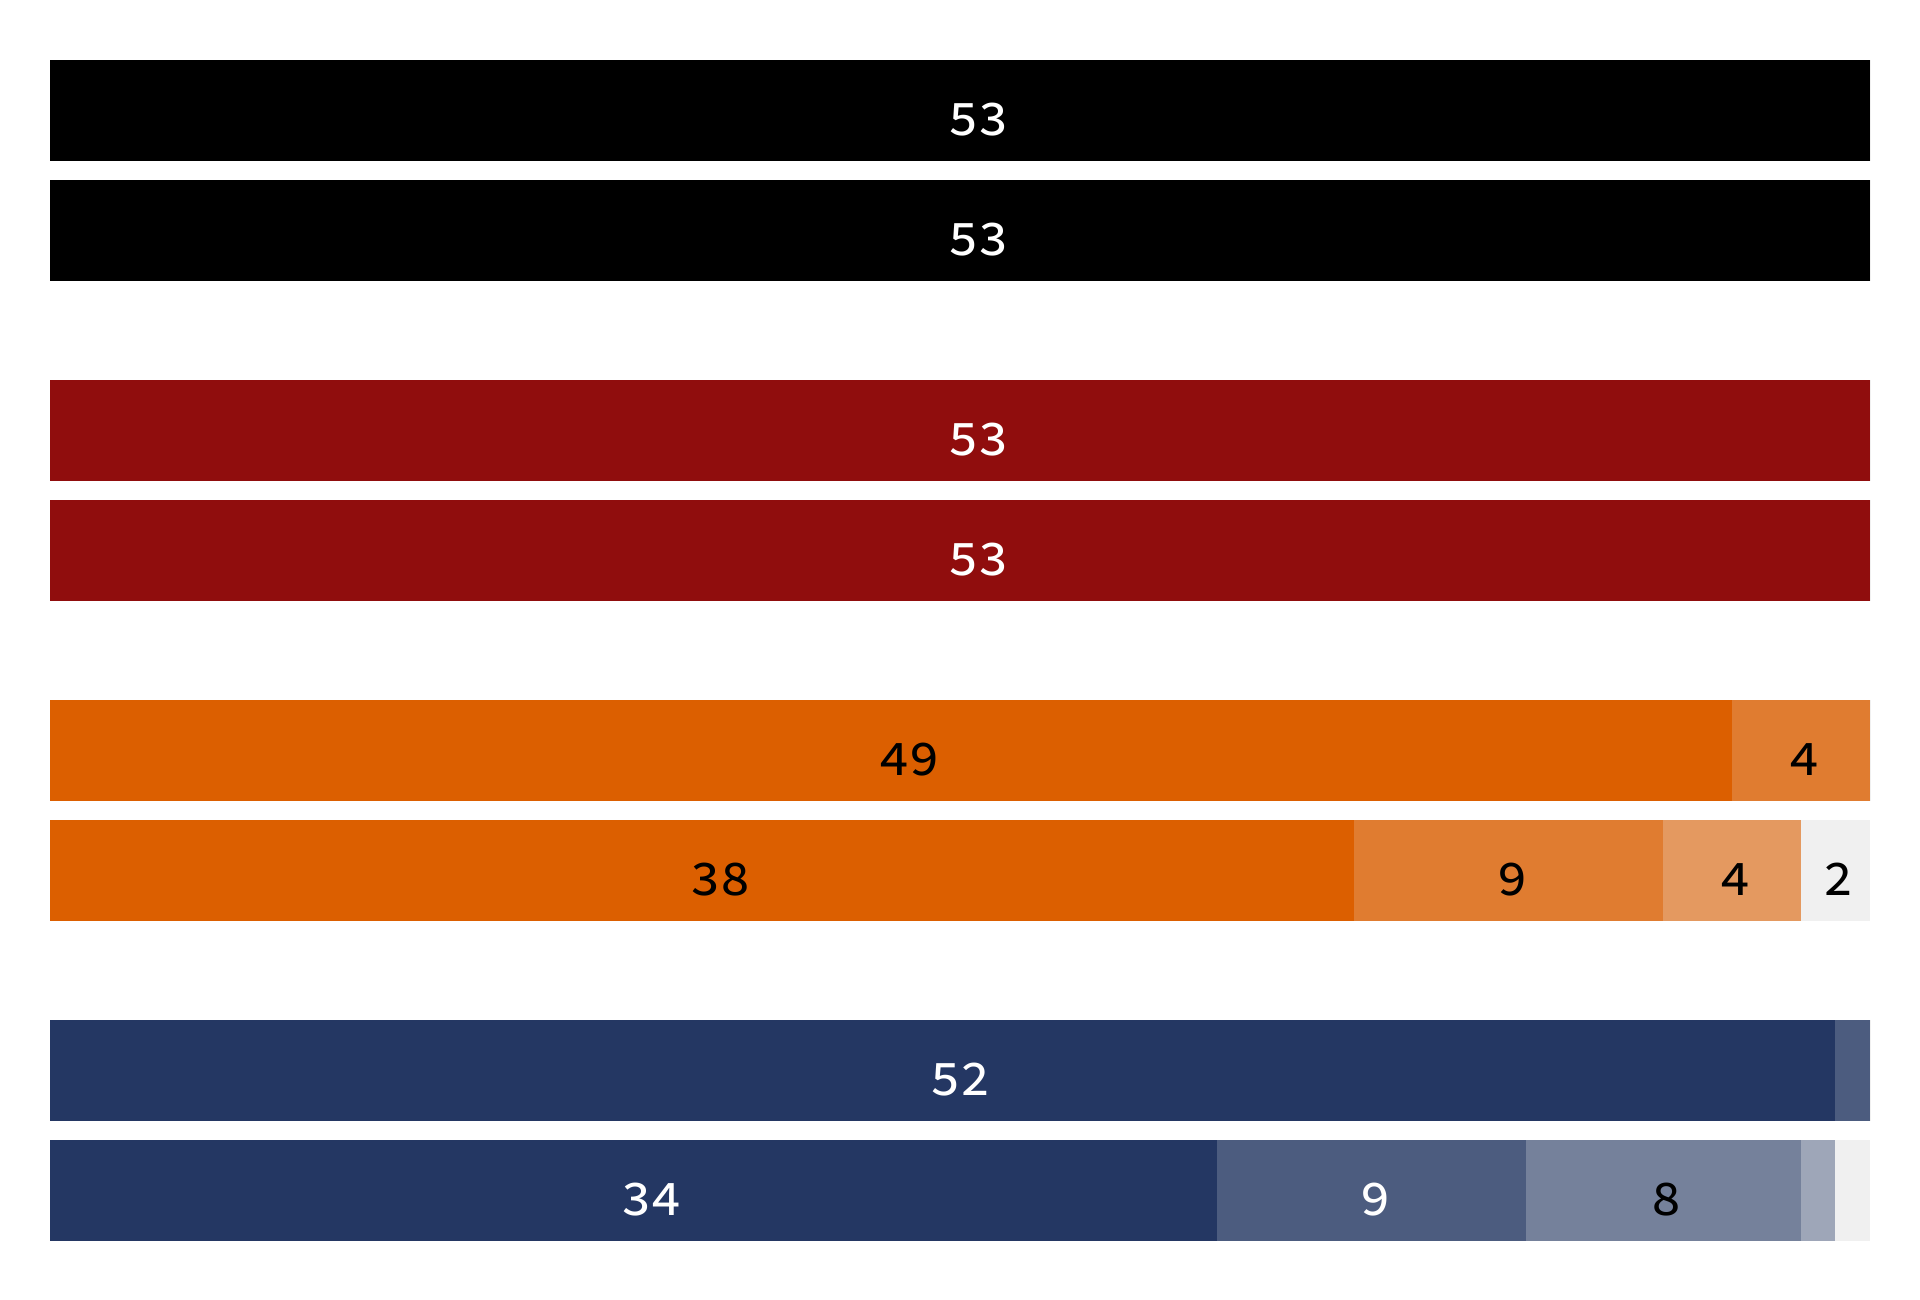
\includegraphics[width=.8\linewidth]{figures/shallow-vs-deep/rocq/BST.png}
    \caption{Binary Search Trees}
    \label{fig:bst_rocq}
  \end{minipage}%
  \begin{minipage}{.5\textwidth}
    \centering
    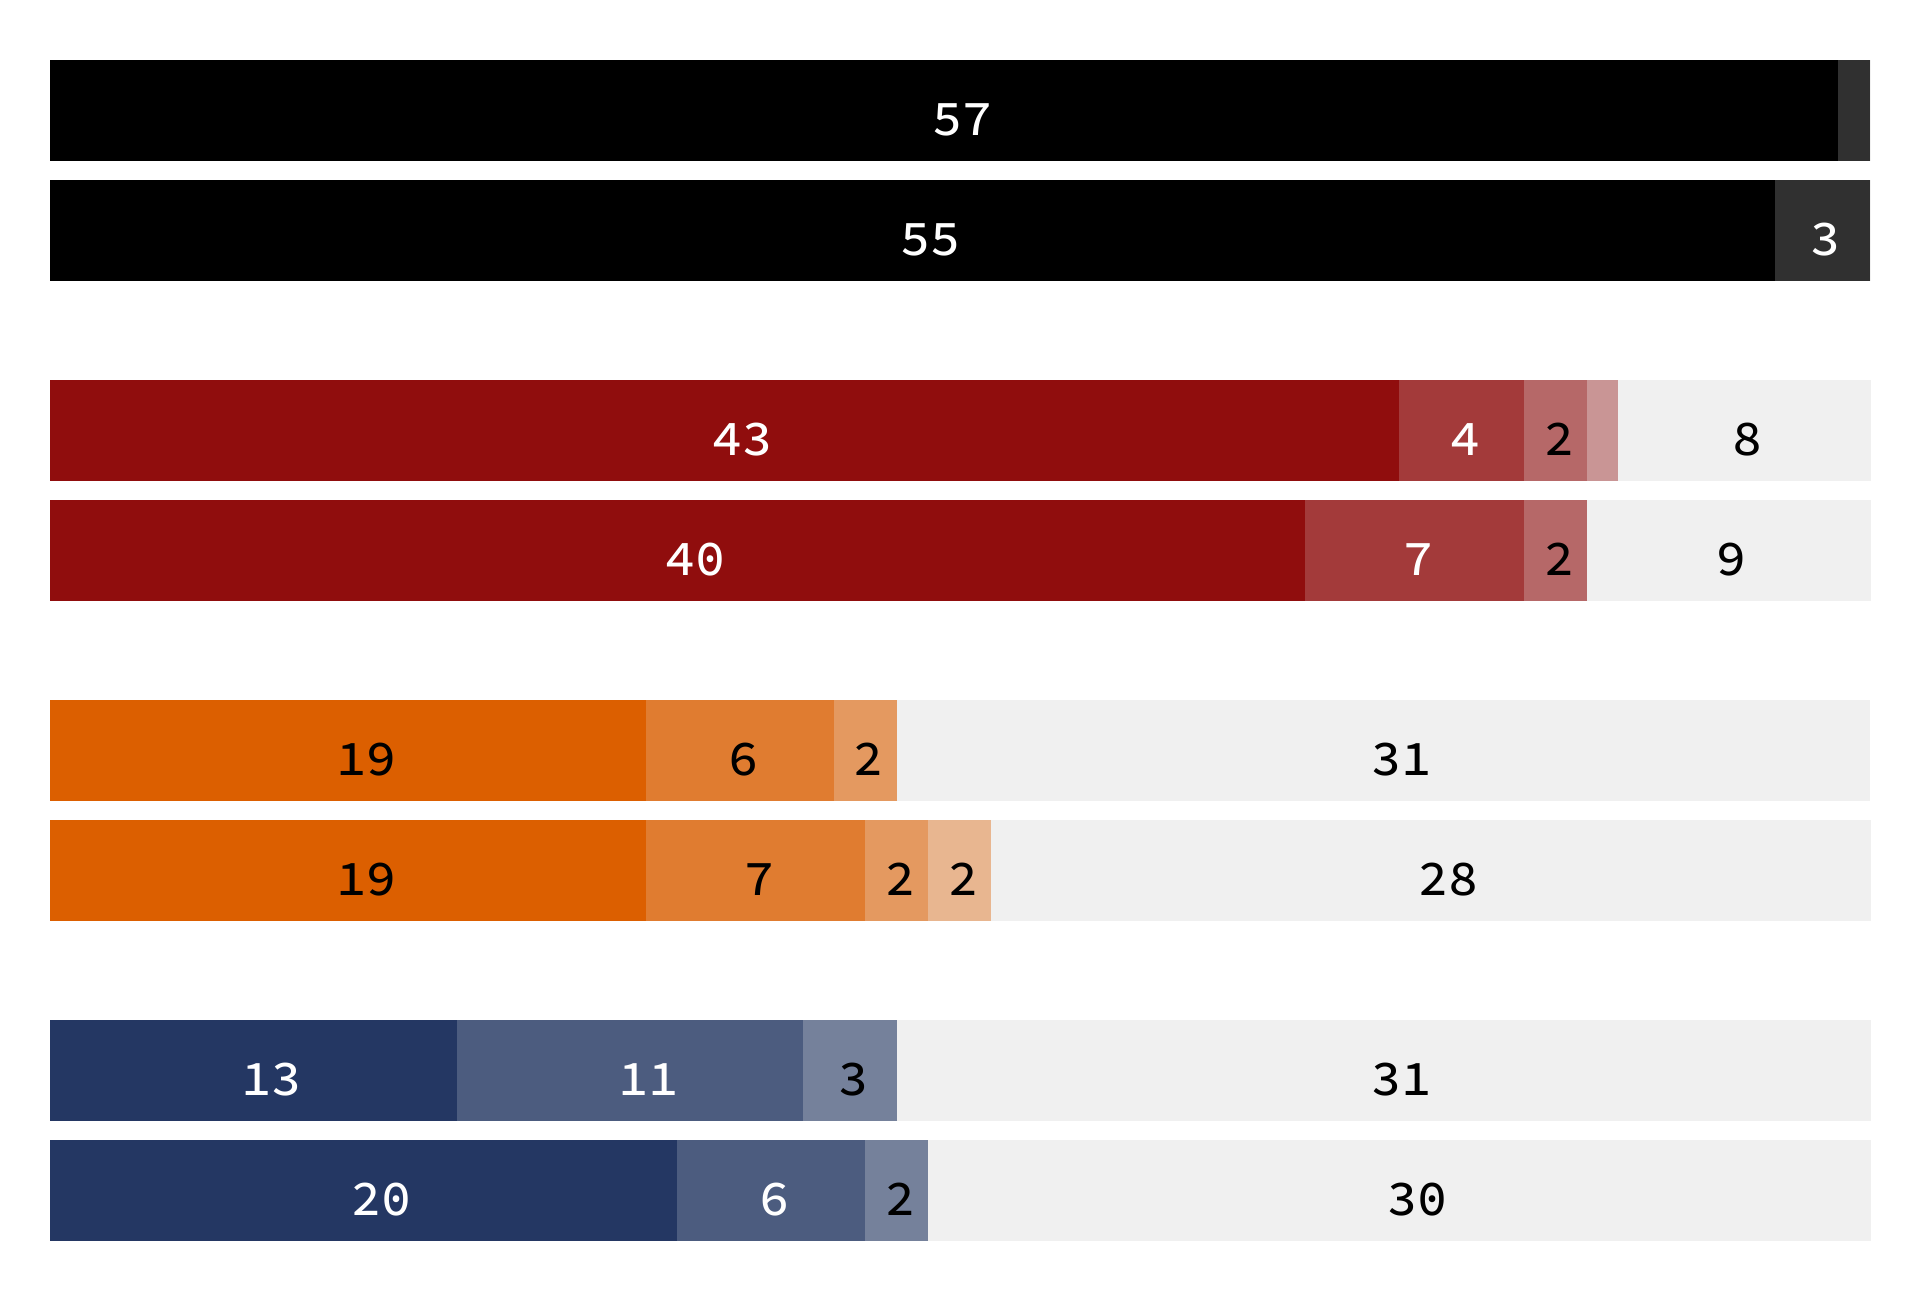
\includegraphics[width=.8\linewidth]{figures/shallow-vs-deep/rocq/RBT.png}
    \caption{Red-Black Trees}
    \label{fig:rbt_rocq}
  \end{minipage}%

  \begin{minipage}{.6\textwidth}
    \centering
    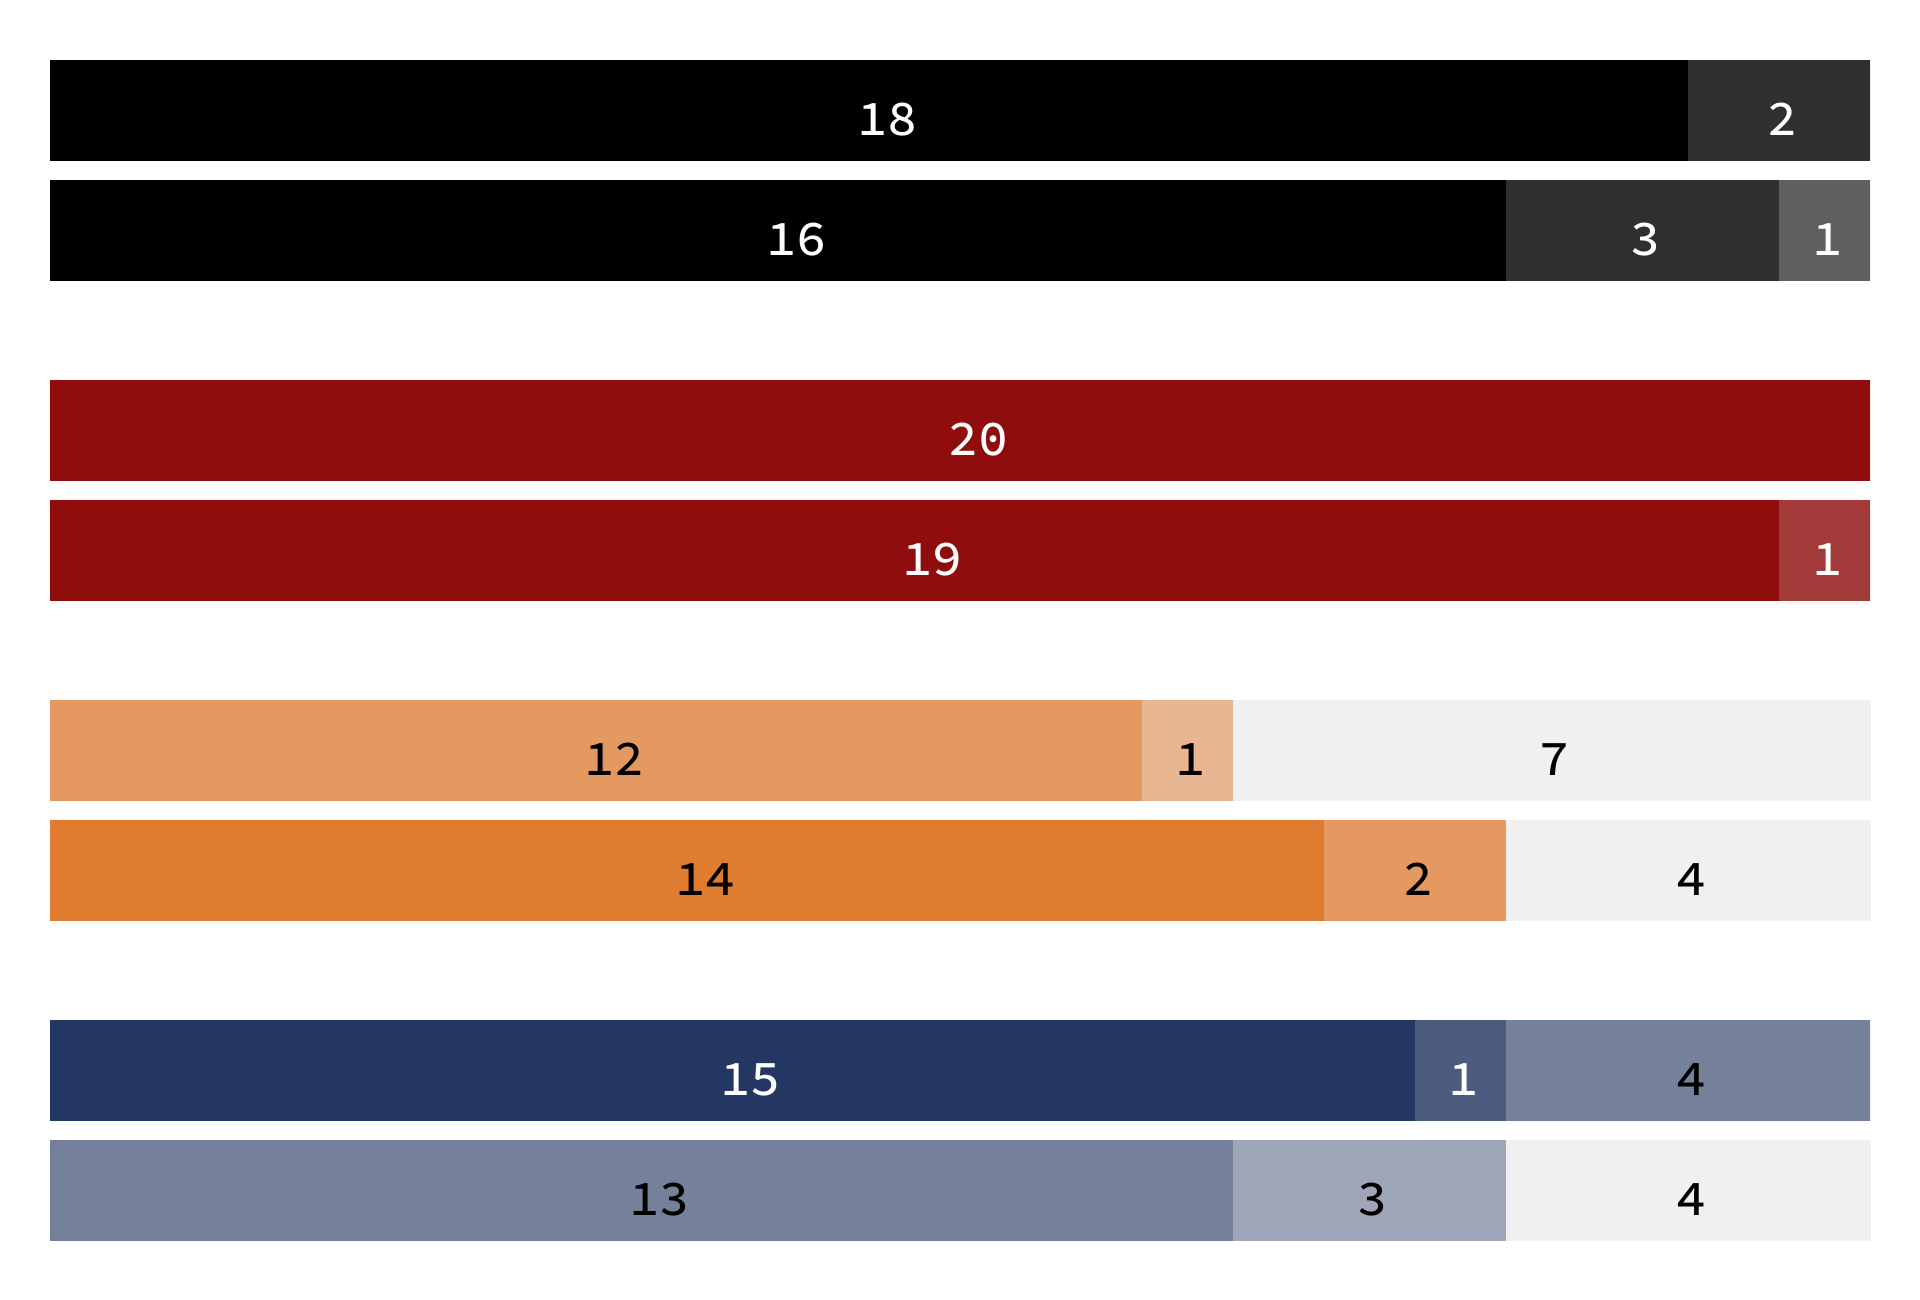
\includegraphics[width=.8\linewidth]{figures/shallow-vs-deep/rocq/STLC.png}
    \caption{Simply-Typed Lambda Calculus}
    \label{fig:STLC_rocq}
  \end{minipage}%
  \captionsetup{justification=centering}
  \caption[Comparison of shallow and deep embeddings in Rocq]{Comparison of shallow and deep embeddings in Rocq. Within each strategy
    color, the top row is the DBAS/deep version and the bottom row is the shallow
    QuickChick version.\\
    \explaincolor{chart_black}{Bespoke generator},
    \explaincolor{chart_red}{Specification-based generator},\\
    \explaincolor{chart_orange}{Type-based fuzzer},
    \explaincolor{chart_blue}{Type-based generator}.}
  \label{fig:shallow_vs_deep_rocq}
\end{figure}

\subsubsection{Comparison of Deep and Shallow Embeddings in Racket}\label{sec:shallow_vs_deep-racket}

In the Racket experiments, we focused on comparing the DBAS-style Racket library with
the shallow embedding implemented by RackCheck. We have conducted our experiments on
the same BST, RBT, and STLC workloads by porting the existing workloads in Haskell to
Racket. In the process of porting these workloads, we have also discovered and reported
\href{https://web.archive.org/web/20260510181513/https://github.com/Bogdanp/rackcheck/issues/14}{a
  bug in the RackCheck core}, which the authors have fixed in the latest version of the
library.

Our Racket results for deep versus shallow embeddings show that, once again, we find no
notable differences in performance between the two versions. However, during the course
of these experiments we found that the default configuration of RackCheck in terms of
size of generated terms led to considerable performance degradation in the RBT case
study. As size is configurable in most PBT APIs, we have changed the RackCheck size
function to be logarithmic with respect to number of tests, as our property-runner
does. Still, this further reinforces our point on programmability: if sizes and similar
aspects of generation are configurable (and severely impact testing performance), why
shouldn’t the runners themselves be configurable?

\begin{figure}[h!]
  \centering
  \begin{minipage}{.50\textwidth}
    \centering
    
\includegraphics[width=.99\linewidth]{figures/shallow-vs-deep/racket/BST_threeway.png}
    \caption{BST}
    \label{fig:bst_racket}
  \end{minipage}%
  \begin{minipage}{.50\textwidth}
    \centering
    
\includegraphics[width=.99\linewidth]{figures/shallow-vs-deep/racket/RBT_threeway.png}
    \caption{RBT}
    \label{fig:rbt_racket}
  \end{minipage}%

  \begin{minipage}{.50\textwidth}
    \centering
    
\includegraphics[width=.99\linewidth]{figures/shallow-vs-deep/racket/STLC_threeway.png}
    \caption{STLC}
    \label{fig:STLC_racket}
  \end{minipage}%
  \captionsetup{justification=centering}
  \caption[Comparison of shallow and deep embeddings in Racket]{Comparison of shallow and deep embeddings in Racket.\\
    \explaincolor{chart_proplang}{DBAS-style Racket},
    \explaincolor{chart_green}{RackCheck}.}
  \label{fig:shallow_vs_deep_racket}
\end{figure}

\subsection{DBAS-powered Experiments}

In this section, I go through three case studies that the expressiveness of DBAS
enabled us to carry out.

\subsubsection{An Exploration of Seed Pool Design Choices}\label{sec:seedpool}

First, we turn to feedback-guided property runners and their programmability. Fuzzing
research often explores different strategies and power schedules~\cite{aflplusplus,
  10.1145/3551349.3559550,DBLP:conf/sigsoft/BohmeMC20, DBLP:journals/tse/BohmePR19}, with
researchers coming up with better and better designs. On the other hand, property-based
testing frameworks that support feedback-guided generation of inputs such as FuzzChick
or Hypothesis, pride themselves in the power of testing arbitrary user-defined
specifications, but do not provide an option to configure such crucial parameters of
their feedback-guided property runners. I illustrated such a feedback-guided runner
earlier in this section, that abstracts away such concerns into a small API, which we
implemented in Rocq.

The configurability enabled by DBAS allows the users to rely on a set of
community-accepted defaults chosen by framework developers, but also to explore if
different choices from the literature or novel ones they devised fit their testing
needs better. In this case study, we explored six different data structure
representations to hold interesting seeds, as well as four different power schedules,
leading to a total of 21 different configurations. We picked these configurations to
explore different parts of the design space, such as the queuing strategy, the
size/cardinality of the pool, whether the pool is monotonic, and how many times a given
seed is reused. We have conducted our experiments on the IFC workload in ETNA, and we
have used a type-based generator alongside a type-based mutator to conduct our
experiments. While this experiment reveals a clear winner for this case study, the
primary goal is not the exploration itself, but rather to demonstrate that such an
exploration can be expressed by varying reusable runner components without modifying
the property language or framework internals.

More concretely, we explored the following data structure representations, three that
hold collections of seeds (as in FuzzChick), and three that only hold a single seed (as
in Targeted PBT):

\begin{enumerate}
  \item {\em FIFO Queue Seed Pool}: A pool that holds a
        queue of seeds, and reduces the energy of the current seed after
        usage.  The pool only generates a new seed from scratch when the
        queue is empty, and mutates the seed otherwise. When the energy of
        the current seed drops to 0, it is removed from the queue. The next
        seed is chosen from the front of the queue. This was the default
        behavior of FuzzChick.

  \item {\em FILO Queue Seed Pool}: The same as the {\em FIFO Queue
            Seed Pool}, but the next seed is chosen from the back of the queue.

  \item {\em Heap Seed Pool}: Similar to the FIFO and FILO Queues, but
        the seeds are stored in a heap, creating a priority queue.

  \item {\em Static Singleton Pool}: A pool that holds a single seed,
        and does not reduce its energy after usage.  The pool generates a
        new seed from scratch at the first iteration, and mutates its seed
        for the subsequent iterations.  The seed is only updated when a new
        seed with a better feedback is generated via mutation. This
        essentially devolves the search to hill climbing, as in the original
        Targeted PBT work~\cite{TargetedPBT}.

  \item {\em Dynamic Monotonic Singleton Pool}: A pool that holds a single
        seed, and reduces its energy after usage.  The pool generates a new
        seed from scratch at the first iteration and when the energy of the
        current seed is 0, mutates the seed otherwise. The seed is only
        updated when a new seed with a better feedback is generated.

  \item {\em Dynamic Resetting Singleton Pool}: A pool that holds a single
        seed, and reduces its energy after usage.  As opposed to the {\em
            Dynamic Monotonic Singleton Pool}, once the current seed's energy is
        0, the seed is effectively discarded and a new seed is generated
        from scratch.

\end{enumerate}

All of the queues except the {\em Static Singleton Pool} have been tested with 4
different energy schedules, where the energy of a new seed was respectively up to 1,
10, 100, 1000, depending on its interestingness. We report the experiments over 5
trials for each configuration within 65 tasks in the IFC workload in ETNA. For brevity,
the graphs omit 34 tasks none of the configurations have solved, and only show the
remaining 31 tasks. Each bucket represents the tasks solved within a certain time limit
for at least one of the 5 trials, where the leftmost bucket with the darkest color
denotes the tasks solved within 0.1 seconds, where the remaining buckets progressively
denote the tasks solved within 1, 10, 60 seconds, and the last bucket denotes the tasks
that were not solved within 60 seconds.

\begin{figure}[h!]
  \centering
  \begin{minipage}{.50\textwidth}
    \centering
    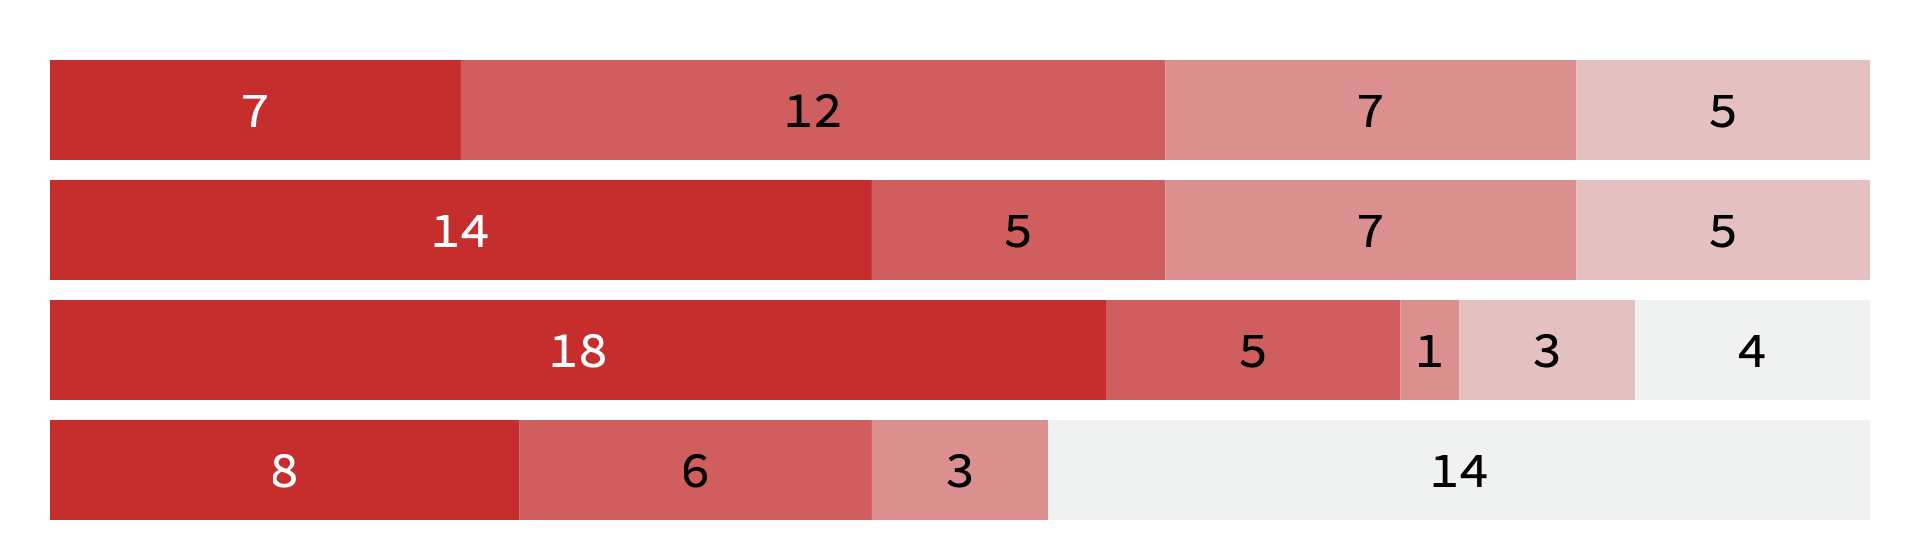
\includegraphics[width=.95\linewidth]{figures/seedpool/HeapSeedPool.png}
    \caption{Heap Seed Pool}
    \label{fig:heapseedpool}
  \end{minipage}%
  \begin{minipage}{.50\textwidth}
    \centering
    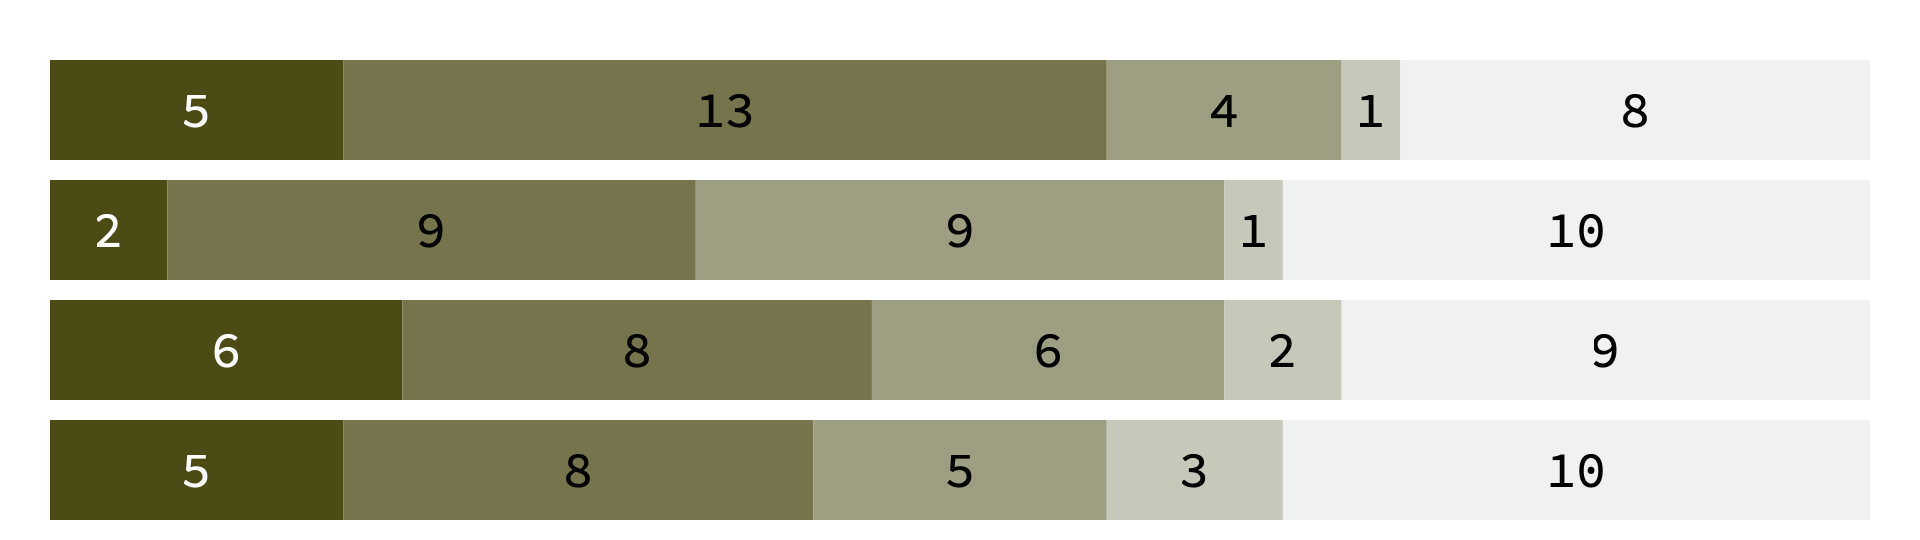
\includegraphics[width=.95\linewidth]{figures/seedpool/FILOSeedPool.png}
    \caption{FILO Queue Seed Pool}
    \label{fig:filoseedpool}
  \end{minipage}%

  \begin{minipage}{.50\textwidth}
    \centering
    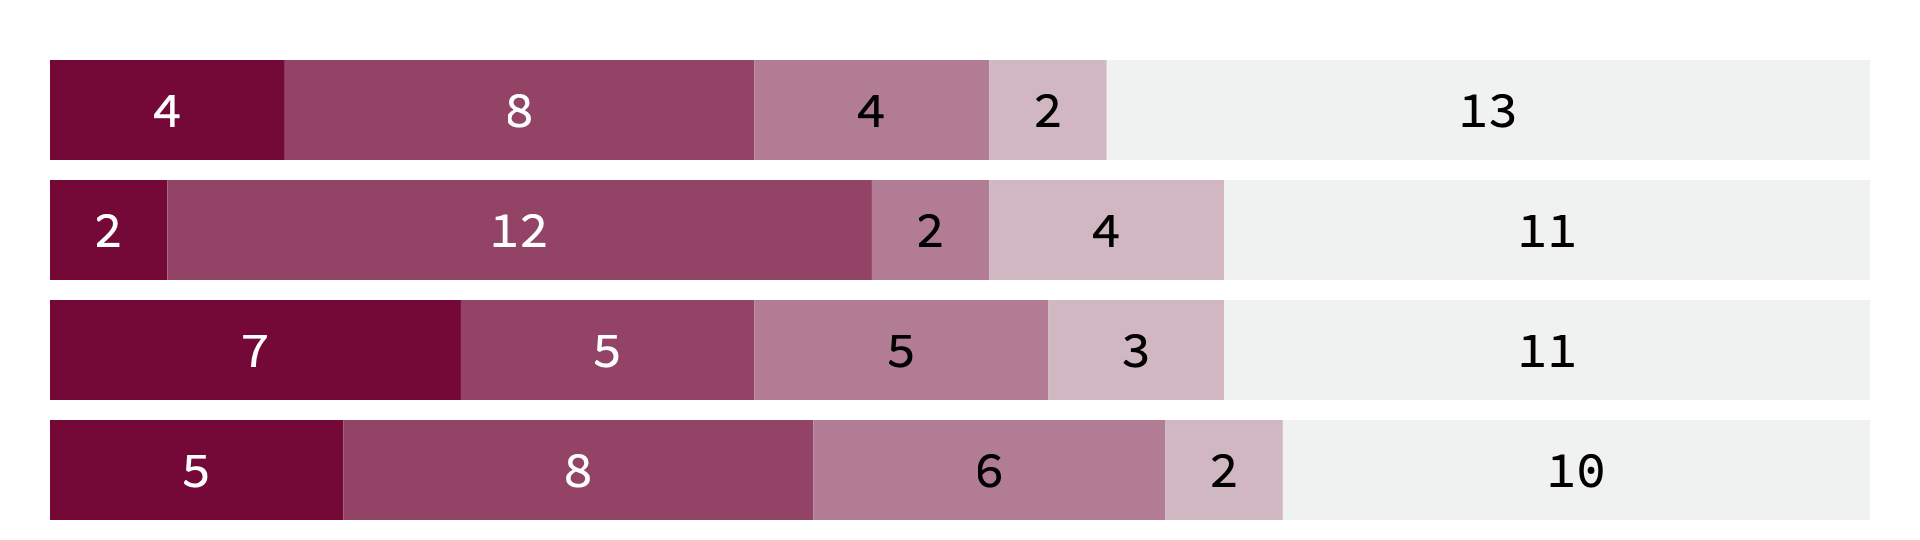
\includegraphics[width=.95\linewidth]{figures/seedpool/FIFOSeedPool.png}
    \caption{FIFO Queue Seed Pool}
    \label{fig:fifo_seedpool}
  \end{minipage}%
  \begin{minipage}{.50\textwidth}
    \centering
    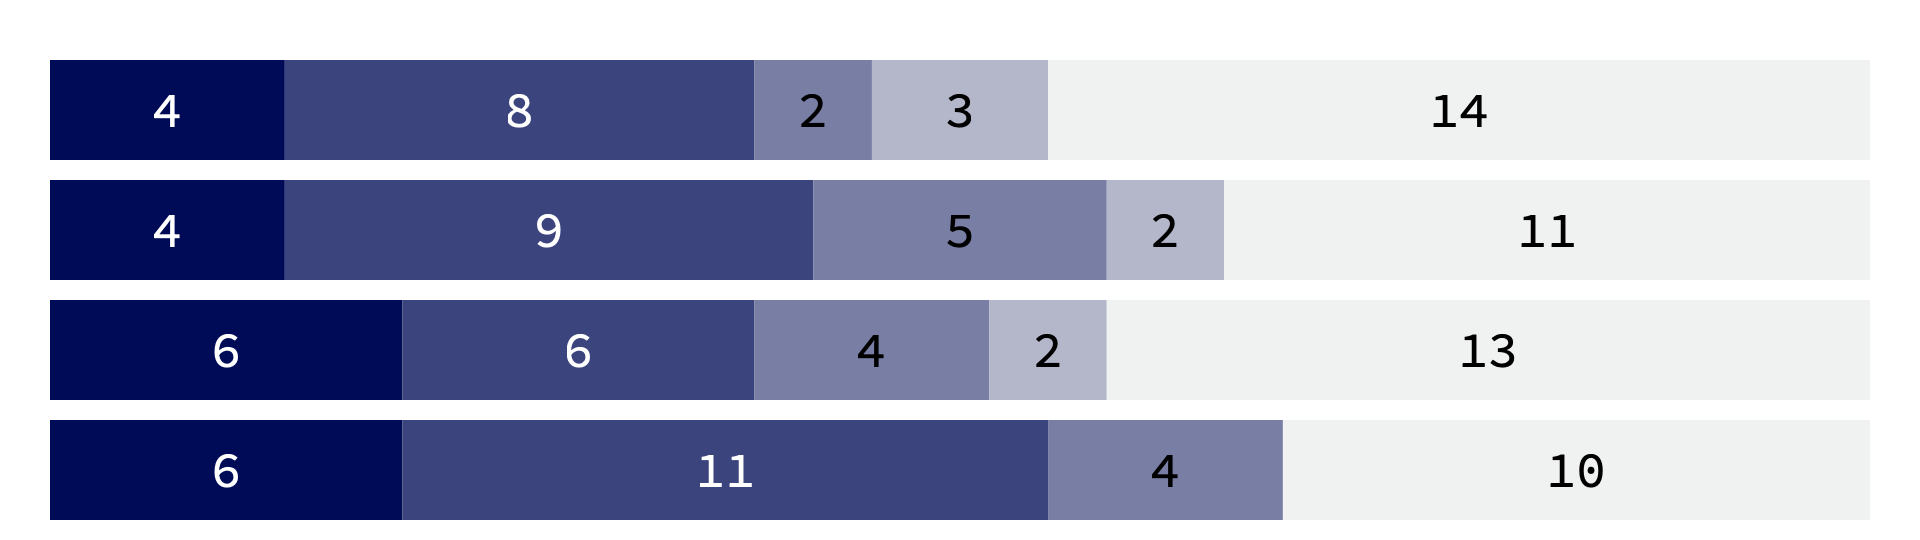
\includegraphics[width=.95\linewidth]{figures/seedpool/DynamicMonotonicSingletonPool.png}
    \caption{Dynamic Monotonic \\ Singleton Seed Pool}
    \label{fig:dynamicmonotonicseedpool}
  \end{minipage}%

  \begin{minipage}{.50\textwidth}
    \centering
    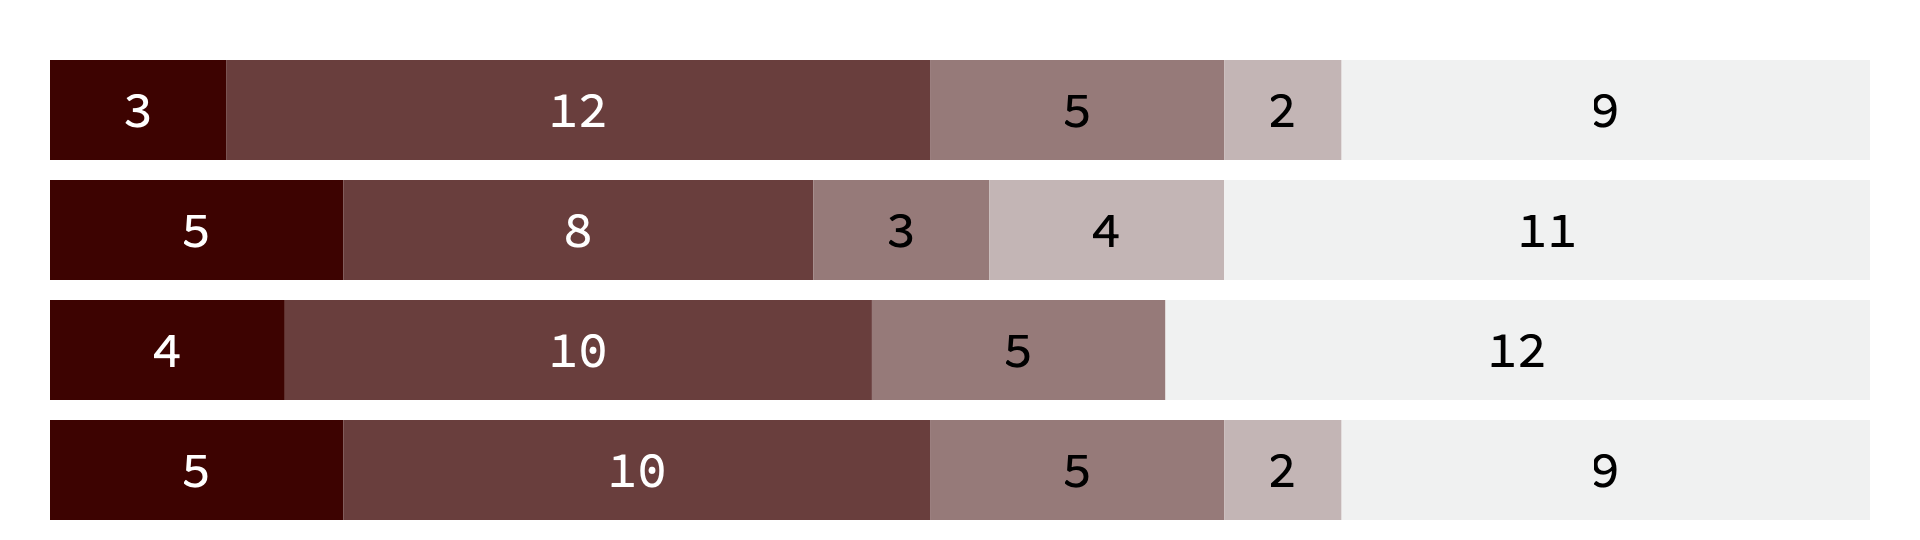
\includegraphics[width=.95\linewidth]{figures/seedpool/DynamicResettingSingletonPool.png}
    \caption{Dynamic Resetting \\ Singleton Seed Pool}
    \label{fig:dynamicresettingseedpool}
  \end{minipage}%
  \begin{minipage}{.50\textwidth}
    \centering
    
\includegraphics[width=.95\linewidth]{figures/seedpool/StaticSingletonPool.png}
    \caption{Static Singleton \\ Seed Pool}
    \label{fig:staticsingletonpool}
  \end{minipage}%
  \caption[Comparison of seedpool strategies in Rocq]{Comparison of seedpool strategies in Rocq. Within each subfigure, rows show
    maximum seed energies 1, 10, 100, and 1000 from top to bottom; the static
    singleton pool has only one configuration. Bucket shading follows
    Figure~\ref{fig:etna-legend}.}
  \label{fig:seedpool_rocq}
\end{figure}

These results mark a task as ``solved'' for the purposes of a bucket chart if at least
1 out of 5 fuzzing campaigns finds a bug. If we switched to requiring {\em all} fuzzing
campaigns to find the bug, the results paint an even more compelling argument: {\em
only} Heap-based pools consistently find counterexamples---I've omitted the graphs
because all other options fail to consistently solve a task across runs, indicating a
very high variance that heap seed pool does not exhibit. As a result, we plan to
upstream the Heap-based seed pool to QuickChick as the effective configuration as a
default going forward.

\subsection{Comparison of Integrated Shrinking with External Shrinking}\label{sec:shrink-comp}

Test case reduction, or counterexample minimization, or shrinking, is a fundamental
aspect of random testing~\cite{zeller2002simplifying}, however it garners much less
attention than its random generation counterpart. A major splitting point in PBT
frameworks has been their approach to shrinking, with the original QuickCheck using
delta-debugging style structural shrinking where the generated counterexample structure
is shrunk by removing its substructures to produce smaller versions with an
accompanying reproducer that tests if the smaller versions keep triggering the bug; and
Hypothesis~\cite{HypothesisShrinking} in Python, falsify~\cite{falsifyLeo2023} in
Haskell, and RackCheck~\cite{rackcheck} in Racket use an alternative route, instead of
shrinking the generated structure, they shrink the source of randomness that led to the
generation. This method, called integrated or internal shrinking, removes the
requirement of a separate shrinking function and preserves the generation invariants in
the generator while making no guarantees on the similarity of the shapes obtained in
the shrinking phase.

The argument, as is the central point of the study, is that such splitting points
should not be decisions at the level of the library, but rather decisions to be made in
relevant contexts by the users of the library. In an ideal scenario, a user should be
able to switch between using an integrated shrinker versus an external one, and vice
versa; and perhaps even use or build a new approach that might not be available when
the library was written in the first place. Instead of forcing the users to choose or
change libraries based on their context and approach to shrinking, DBAS allows for
building your own property runner with its custom approach to shrinking, and that is
precisely what we have done in this experiment.

We have compared the effectiveness of the integrated shrinker of RackCheck against a
simple external shrinker we have implemented in our DBAS PBT library in Racket. We have
conducted our experiment on the {\tt System F} workload in ETNA, and we used the same
generator in both RackCheck and DBAS-style Racket library, equipping our library with a
simple type-based external shrinker we implemented in place of the integrated shrinker.

The results show that the external shrinker successfully shrinks System F terms to a
minimal counterexample that is an average of 2.66 times smaller than the original input
with a standard deviation of 1.23, while the integrated shrinker of RackCheck only
shrinks the inputs to an average rate of 1.04 times smaller than the original input
with a standard deviation of 0.37. RackCheck only shrunk the inputs to smaller inputs
in 66 out of the 360 trials, kept the size the same in 77, grew the inputs in 68, and
failed to shrink in 149 trials. These results may be surprising at first glance: does
the internal shrinker really only shrink the inputs in 20\% of the trials? In this
case, it does. Its notion of size is based on the structure of the generator rather
than on the input itself, so ``smaller randomness'' may not actually lead to smaller
input values.

The point of this experiment is not to demonize internal shrinking---for many testing
situations, it is perfectly sufficient and much more user-friendly than a bespoke
shrinker. However, in pathological cases, programmers need an escape hatch, and DBAS
provides the necessary configurability.

\begin{figure}[h!]
  \centering
  \begin{minipage}{.5\textwidth}
    \centering
    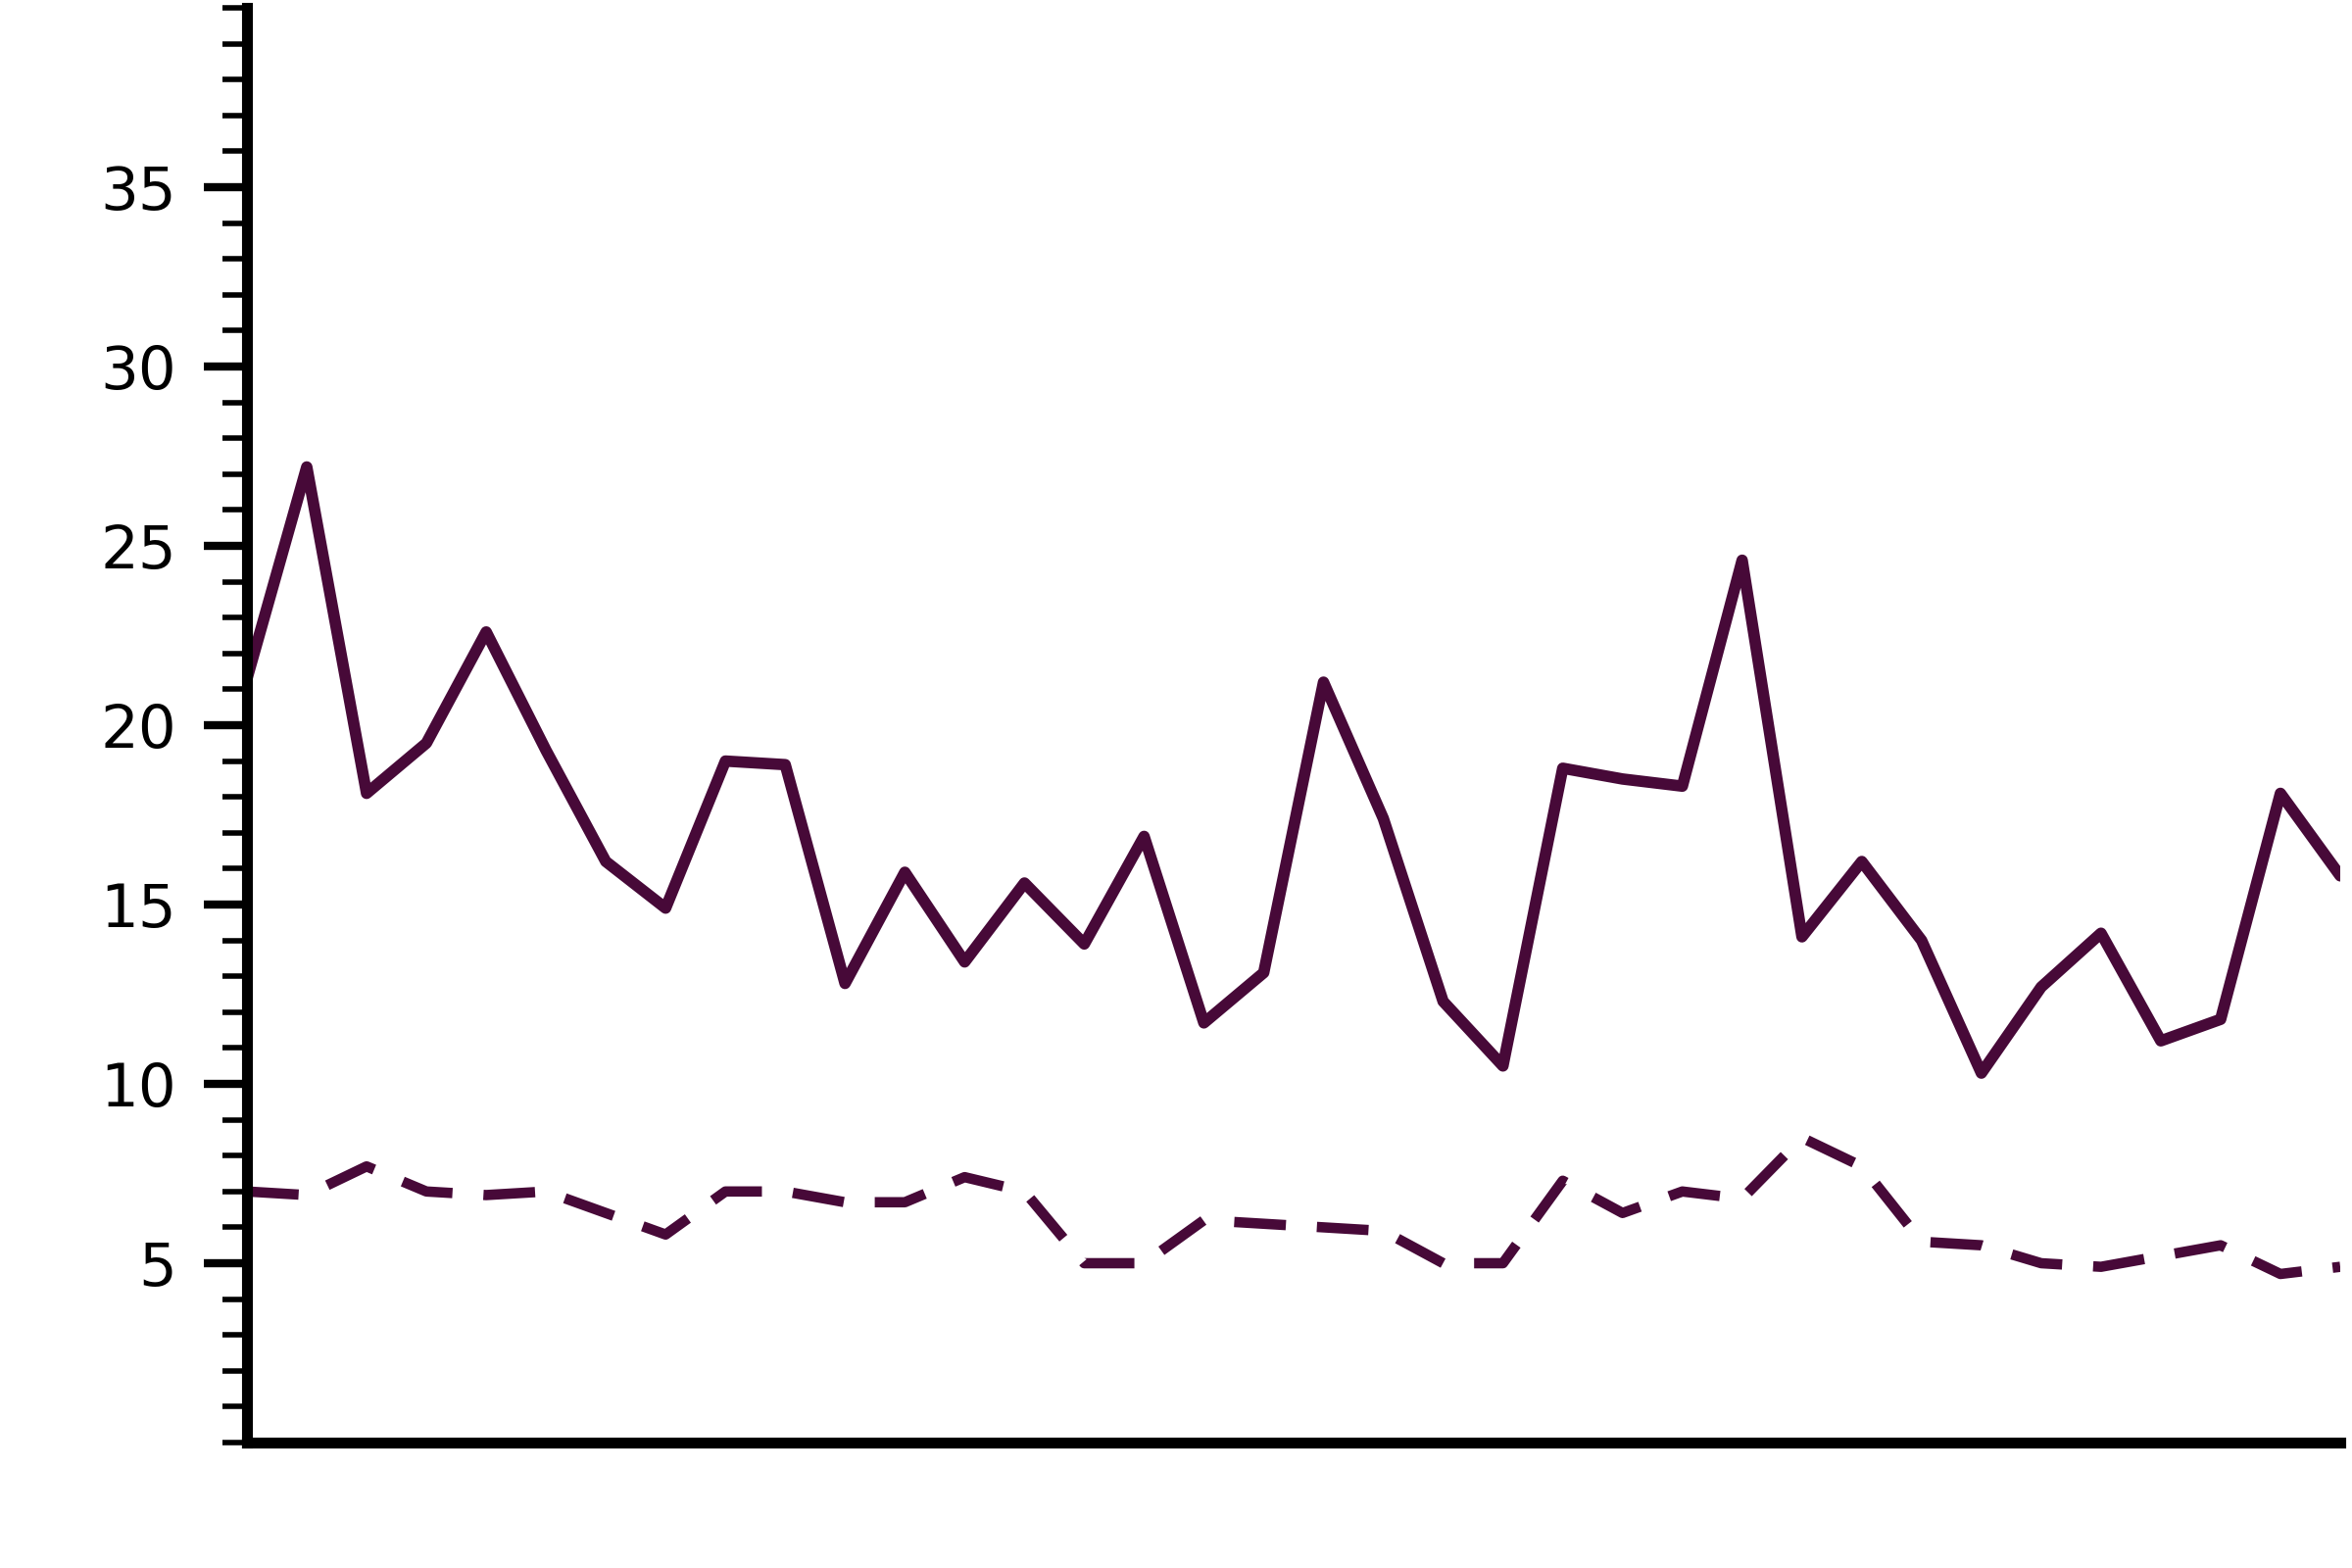
\includegraphics[width=0.9\linewidth]{figures/shrinking/scatter_plot_proplang.png}
  \end{minipage}%
  \begin{minipage}{.5\textwidth}
    \centering
    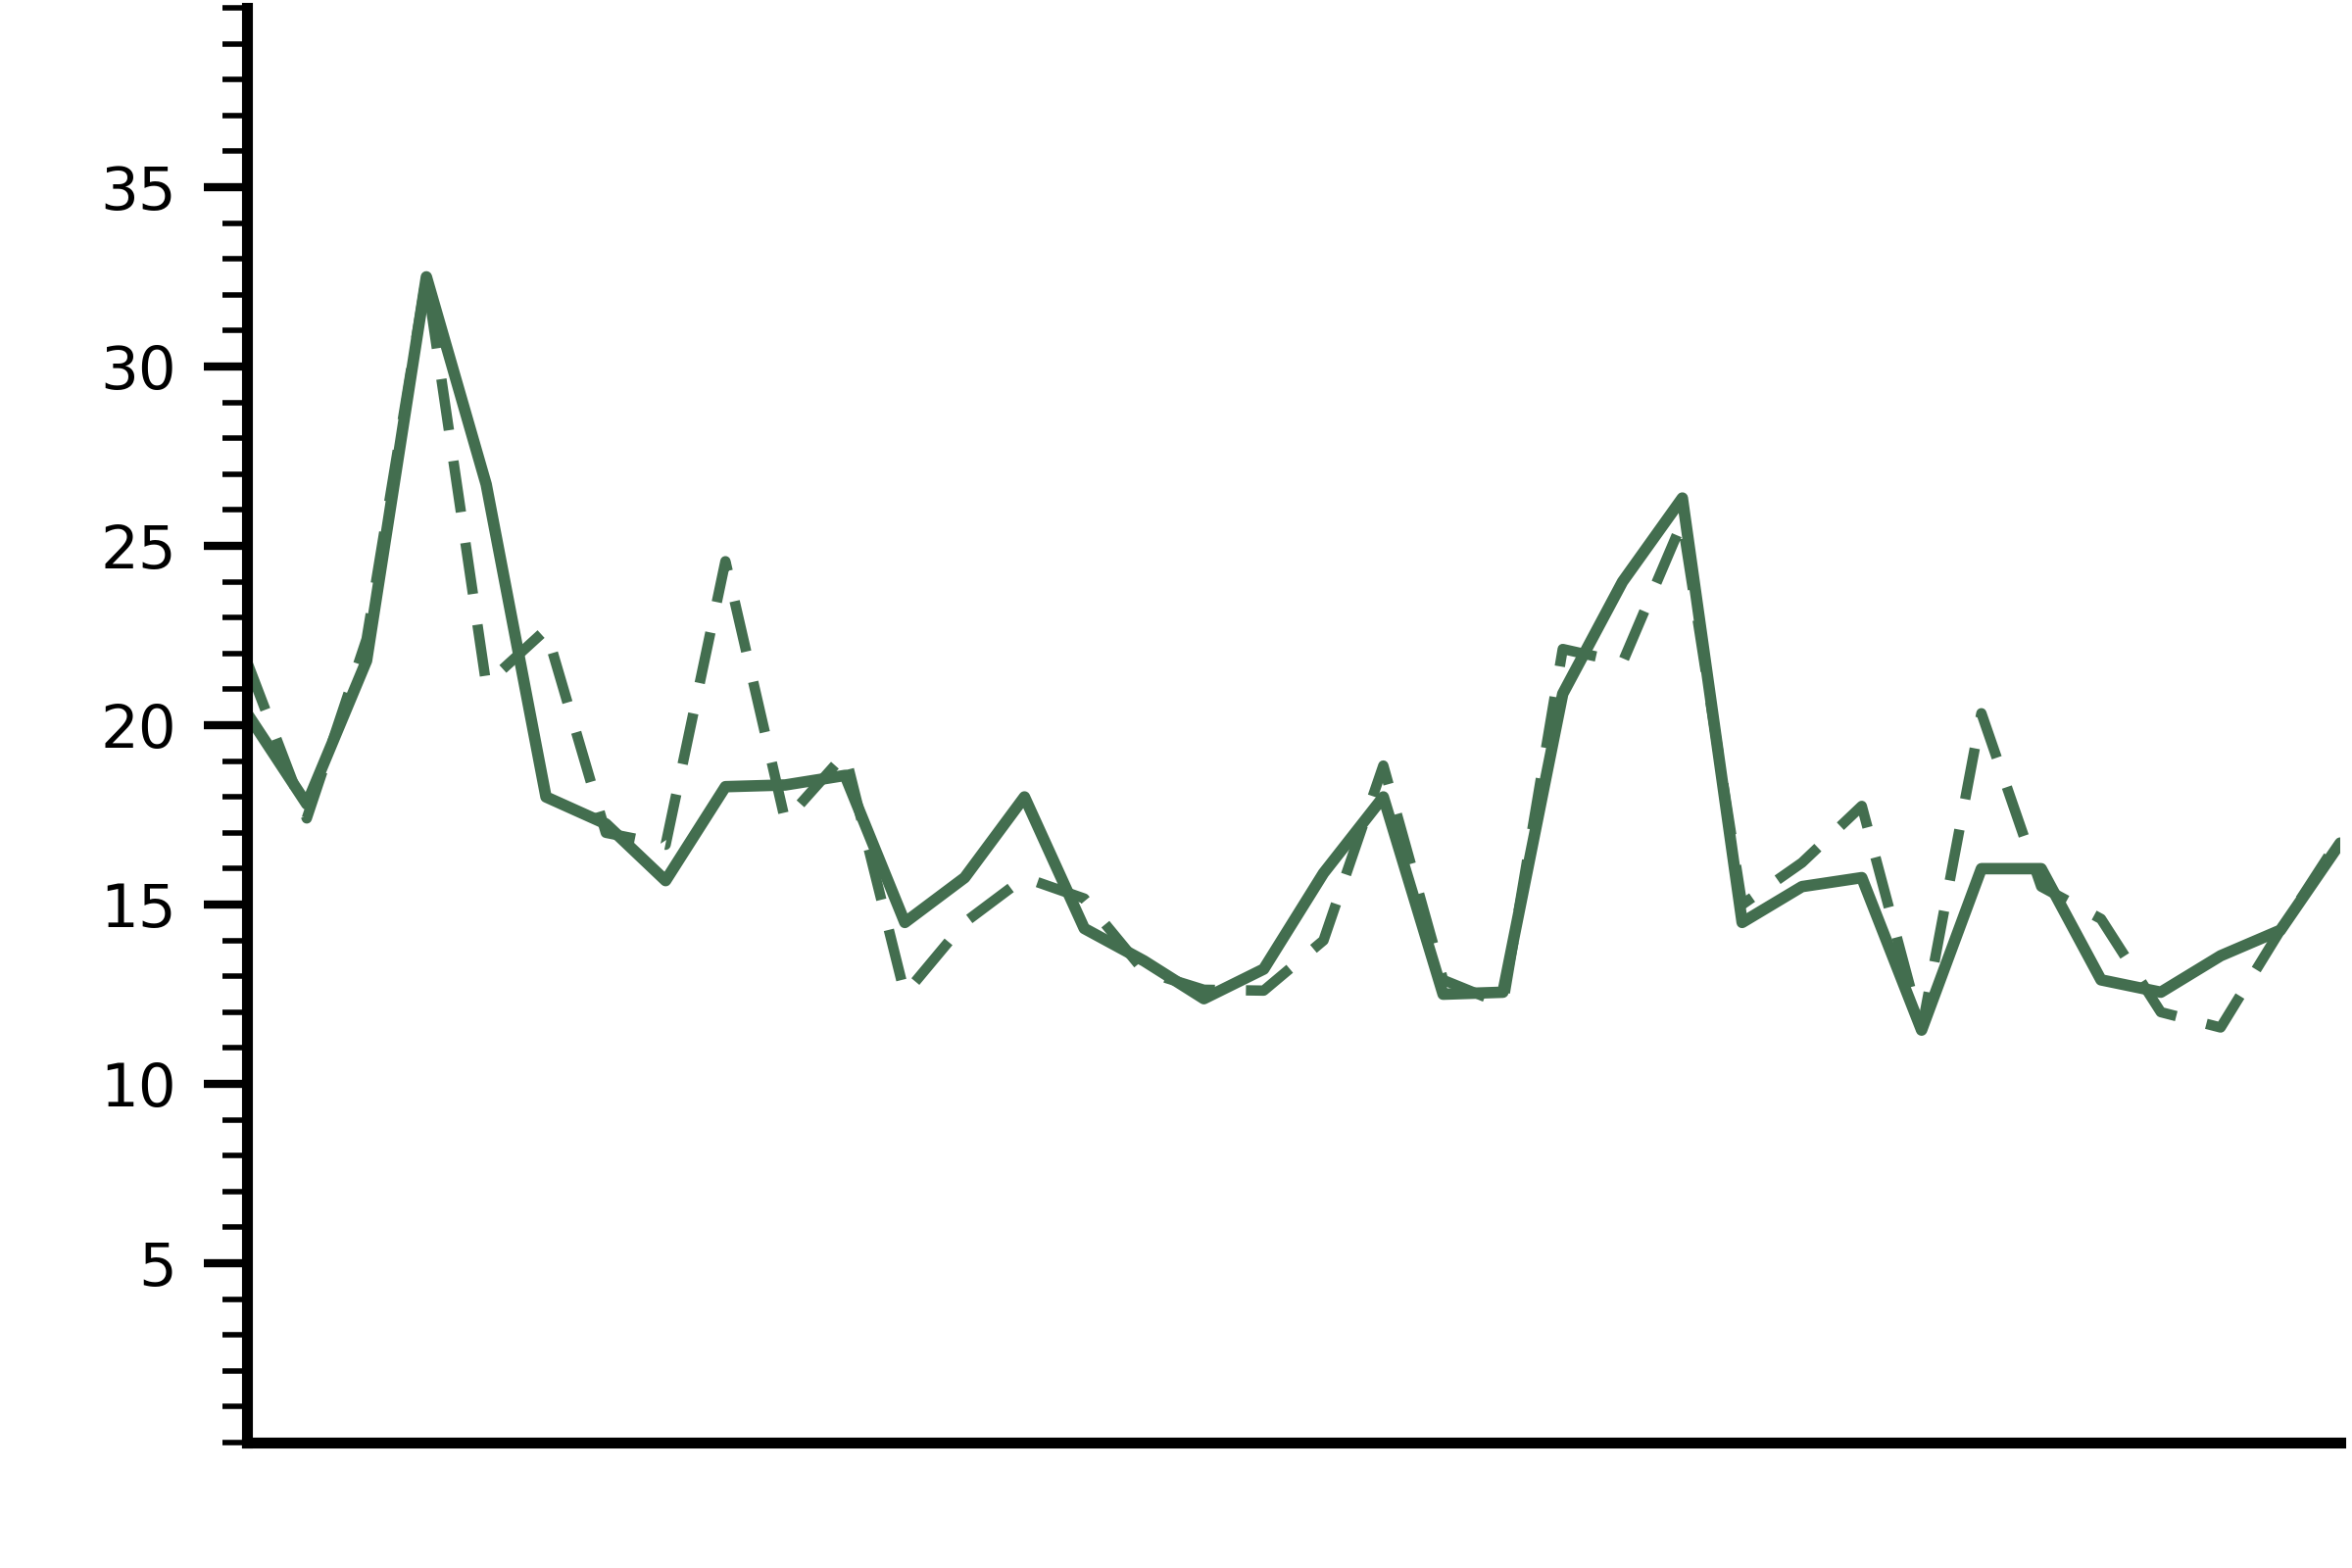
\includegraphics[width=0.9\linewidth]{figures/shrinking/scatter_plot_rackcheck.png}
  \end{minipage}%
  \caption[Comparison of shrinking in DBAS vs RackCheck.]{Comparison of shrinking in DBAS vs RackCheck.\\ Original sizes (continuous) and shrunk sizes (dashed) across tasks (x axis)
    for the external shrinker (left) and internal shrinker (right).}
  \label{fig:shrinking_line}
\end{figure}

\subsection{Parallelizing Property-Based Testing} \label{sec:parallel-experiment}

An important recent work on novel property runners is
QuickerCheck~\cite{ParallelTesting}, where authors implement and evaluate a parallel
run-time for QuickCheck~\cite{ClaessenH00}, achieving massive performance gains on a
variety of workloads as opposed to prior work leveraging parallelism by producing a
swarm of testing configurations~\cite{swarm-testing}. The underlying idea the authors
propose is rather simple, they provide an alternative, parallel property runner {\tt
    quickCheckPar}, where multiple worker threads share a common variable that controls the
size of the generated inputs. Using this strategy, the authors achieve an almost linear
speed-up with respect to the number of physical cores used in testing. Unfortunately,
due to the rigid structure of shallow embedding based PBT libraries, creating such a
parallel runner requires intensive engineering effort. The commit history of the
project shows that the implementation of this new runner is an effort spanning 2 years
and more than 50 commits.

In contrast, the DBAS-style Racket library let us implement a naive version of the
QuickerCheck algorithm as a user-space runner, without changing the property
representation or the core framework. Our implementation uses worker threads with 2
shared atomic variables, one keeping the current number of tests across threads, and
one indicating if the process of testing is finished or not.

We compared this 4-thread parallel runner against the single-threaded runner across 131
tasks (53 BST, 58 RBT, 20 STLC). The result is mixed, which is expected for these
workloads: most ETNA tasks are solved by bespoke Racket generators within 0.1 seconds
(\S~\ref{sec:shallow_vs_deep-racket}), leaving little room for parallelism to overcome
thread-management overhead. Among the 49 tasks where the single-threaded and parallel
times differ by more than one millisecond, the parallel runner is slower on average
(the average time ratio is 1.2, i.e., 20\% more time). On the 10 tasks where the
difference exceeds 0.1 seconds, the parallel runner is faster by roughly 3x on average
(the average time ratio is 0.33). The only task with a difference above one second
takes 3.56 seconds with the single-threaded runner and 1.16 seconds with the parallel
runner. These numbers should not be read as evidence that this naive Racket
implementation matches QuickerCheck's optimized runtime; rather, they show that DBAS
lets a user implement and evaluate a new runner design directly, exposing the expected
trade-off between parallel overhead on tiny tasks and speedup on longer-running ones.

\section{Related Work}\label{sec:related}

Throughout the chapter, I have thoroughly discussed various property-based testing
frameworks, their property languages, and the property runners that they come bundled
with. Here, I briefly summarize related work in PBT and we also discuss related work in
deeply embedded domain-specific languages.

\paragraph{Property-Based Testing Frameworks}

To our knowledge, no widely-used frameworks expose a reified property representation
that supports user-defined runners without modifying library internals. There are
multiple frameworks that make distinctly different choices in what capabilities they
provide to users as presented in Table~\ref{tab:pbt-frameworks}.

\paragraph{Free Generators}

The design of our deeply embedded property language builds on a rich literature of
embedded DSLs~\cite{hudakBuildingDomainspecificEmbedded1996}. In particular, our
approach parallels work on {\em free generators}~\cite{goldsteinParsingRandomness2022},
which present a deeply embedded DSL for writing random generators. Deeply embedded
properties and generators are largely orthogonal---free generators may be able to
simplify the implementation of some of the different runners described in
\S~\ref{sec:eval}, but they do not allow the developer to re-program the loop itself.
%
This follows a more general trend of using free structures to increase expressivity or
usability in the programming languages community. For example,
itrees~\cite{DBLP:journals/pacmpl/XiaZHHMPZ20} introduced a general-purpose Rocq
structure which is essentially a coinductive variant of free monads, which allows them
to represent and reason about interactive recursive programs. In follow up work,
\citet{DBLP:journals/pacmpl/LiW22} explored how other free structures (such as
applicative functors) can be used as an alternative to free-monad-based embeddings.

\paragraph{Mixed Embeddings}
There is also a long line of related work in attempting to bridge the benefits of
shallow embeddings (ease of use, as in the current property language) with those of
deep ones (extensibility). For example, \citet{CARETTE_KISELYOV_SHAN_2009} showed how
to use typeclasses in Haskell to allow for shallow embeddings that can be interpreted
in different ways, hinting at a way of incorporating a deeper property language in a
type system such as Haskell's. More recently, \citet{Unembedding} showed how to convert
between embedding representations by {\em unembedding} alleviating some of the problems
with Higher-Order Abstract Syntax representations. Finally,
\citet{DeeperShallowEmbeddings} introduced a hybrid embedding where typing derivations
are represented as a deep embedding indexed by shallow terms in the host language,
offering pattern matching capabilities.

% \paragraph{DBAS for STLC}
% To conclude the overview of related work, let us contrast once again
% some of the most popular embedding techniques in a more familiar context:
% the simply typed lambda calculus.
% Higher O

\section{Conclusion and Future Work}\label{sec:future}
In this chapter, I have presented Programmable Property-Based Testing, a PBT paradigm
that changes the underlying representation of properties using deferred binding
abstract syntax (DBAS), a mixed embedding we introduce. Programmable PBT is a new
approach to encoding properties for PBT that enables more flexible and programmable
testing. The key advance made by DBAS is to reify properties as a free data structure;
allowing them to be written in a clear and readable way, separate from the property
runner that tests them. These more deeply embedded properties can then be inspected and
interpreted by user-defined property runners. With the help of DBAS, developers in
Rocq, Racket, and hopefully soon other programming languages, can tailor, experiment,
and adapt their testing setup to their domain.

In the future, we intend to make DBAS convenient to program in more mainstream
languages than Rocq and Racket. On the static typing side, we chose to implement our
approach in Rocq as its dependent type system and powerful notation mechanism allowed
us to conveniently express the heterogeneous contexts involved. The same approach
should also be implementable in Haskell using standard GADT-based heterogeneous
lists~\cite{HaskellPromotion}; however, without access to notational conveniences as in
Rocq, it remains future work to see how to regain a similar degree of ergonomics in
that setting. On the dynamic typing side, the techniques described should be readily
transferrable to other languages. For example, given Python's powerful reflection
capabilities and its convenient decorator features, a deferred-binding style property
language should be implementable on top of, e.g., Hypothesis.
% We intend to do more work to
% make \name{} convenient and safe program in in languages with more
% traditional type systems.


\clearpage

\renewcommand{\thechapter}{3}

\chapter{Quantitative Evaluation of Property-Based\\Testing}\label{chap:etna}

The second chapter of this thesis remarks a fragmentation caused by the design of
property-based testing libraries, leading to diverging features, separated ecosystems.
In this chapter, I focus on yet another fragmentation, this time caused by something
much more banal, a lack of general purpose evaluation benchmarks for PBT. The
literature is full of interesting novel techniques for enhancing random generation and
counterexample minimization, but these techniques are rarely evaluated within a
coherent context. Many times, the studies have relied on bespoke benchmarks
(\todo{examples}), if one were to build a web of studies and the benchmarks they used,
the result is somewhat reminiscent of the infamous public transport coverage of Ankara,
a small number of hub workloads that many studies reuse, many one-off benchmarks that
haven't been validated or reused in other studies, and a complete lack of
standardization.

This lack of common comparative analysis surely contributes to a lack of understanding
in the effects of these new techniques and changes; but the problem is persistent
beyond the literature and into the libraries themselves. All the property-based testing
libraries I have read in the course of developing this thesis are full of bespoke
decisions accummulated in the last 25 years. The choice of which sizing function to
use, the shrinking algorithm, the default settings on budgets and parameters... Many of
these decisions have never been subject to quantitative judgement beyond the initial
discussions, never been evaluated at scale, or understood in the broader context of PBT
usage.

In the beginning of my Ph.D. we set out to remediate this fragmentation and help build
a common quantitative understanding for the field. With Jessica and Harry implementing
the common evaluation framework in Python as well as the Haskell workloads, and I
working on the implementation of the Rocq pipeline and workloads, we have published
``Etna: An Evaluation Platform for Property-Based Testing (Experience
Report)''~\cite{etna-icfp23} in ICFP23.

After the initial publication, I have taken the lead role in future development of the
ETNA platform and horizontally grown it for OCaml with Nikhil Kamath, Racket with Ceren
Mert and Justine Frank, for Haskell with George Miao, and for Rust by myself. The
initial implementation as a library has been replaced with a standalone tool that could
be easily run cross-platform on many machines, eventually to the point we can start to
run our experiments as Github Actions. Many of these changes have found their ways into
publications, our JFP extension for the ICFP23 paper has incorporated the work by Ceren
and Nikhil as well as Tin from UPenn working together with Jessica.

The rest of this chapter includes excerpts edited from these papers, mainly the 2026
JFP extension of ETNA, with a major section on evaluation of shrinking from our
under-review work for the Haskell Symposium with George and Leo.

\section{ETNA}

ETNA is, as you may have thought of, named after the famous Sicilian volcano~\cn. The
name follows a convention established by prior work in the fuzz testing community,
Lava~\cite{Lava} and Magma~\cite{Hazimeh:2020:Magma}, both of which have been
instrumental to our design, particularly with the ground truth approach of Magma.

During the design and development of ETNA, we focused on a few key design principles,
centered around usefulness, extensibility, and maintainability.

\subsection{Evaluate for the ground truth, not for proxy metrics.}

How should an evaluation platform measure the effectiveness of a generator? The
software testing literature offers two common answers: \emph{code coverage} and
\emph{mutation testing}. Code coverage is attractive because it is easy to instrument
and compare, but it is at best an indirect signal: higher coverage does not always
translate to better bug finding~\cite{GopinathJG14,EvaluatingFuzzTesting}. For ETNA, we
instead chose mutation testing~\cite{JiaH11}, which measures the effectiveness of a
testing technique by artificially injecting mutations into the system under test and
checking whether testing is able to detect them.

Mutations used in prior evaluation work fall on a spectrum from manually sourced to
automatically synthesized~\cite{Hazimeh:2020:Magma,EvaluatingFuzzTesting,
    FixReverter,TestingNIjfp}. ETNA opts for manual sourcing. This choice makes the
benchmark harder to populate, since every task requires a meaningful mutant and a
property that exposes it, but it also lets us maintain a clearer ground truth: each
mutant should violate some aspect of the property specification. The workloads,
properties, and injected bugs used in this chapter are detailed in
\S~\ref{etna:workloads}.

\subsection{Use minimal, but precise interfaces.}

A key challenge during ETNA's development was that the platform needed to gather
comparable data about the testing effectiveness of a wide variety of existing PBT
frameworks, each of which reports such data in an ad-hoc and non-standardized manner.
Most frameworks report the number of inputs generated before a counterexample is found.
Far fewer expose timing statistics, and none of the frameworks we studied initially
offered a detailed breakdown of generation, testing, and minimization time. Similarly,
most frameworks report the number of inputs that fail to satisfy a precondition as
discards, while others, such as Rust's QuickCheck and Racket's RackCheck, do not
separate discards from passing tests.

These differences matter because ETNA is not evaluating a single library in isolation;
it is trying to compare workloads, strategies, frameworks, and languages. To make those
comparisons meaningful, we settled on a small set of metrics that are easy to measure
across frameworks and on a precise output format that implementations can validate
themselves: JSON conforming to a schema exposed by the ETNA
protocol.\footnote{\url{https://github.com/alpaylan/etna-cli/blob/main/PROTOCOL.md}}
The resulting interface is intentionally modest. It does not try to encode every
feature of every PBT library. Instead, it records the information that ETNA needs to
run experiments reproducibly and compare their outcomes.

\subsection{Every ETNA capability should be available to use manually.}

ETNA acts as an orchestration mechanism: it invokes testing tools, toggles mutations,
parses results, and performs analysis over the collected data. Such orchestration is
fragile even when every component is individually well engineered, because ETNA sits
between loosely coupled systems that were developed independently. In practice, any
opaqueness in this process can make failures difficult to diagnose and, in the worst
case, unrecoverable.

The final guiding principle of ETNA is therefore transparency. Each step of an
experiment should correspond to an operation that a user can understand and, when
needed, reproduce manually. This principle shaped the transition from the initial
library implementation to the standalone command-line tool described in the next
section. Rather than hiding build steps, mutation activation, test execution, and
analysis behind a single opaque pipeline, ETNA exposes them as ordinary commands. That
design makes the platform easier to debug, easier to extend to new languages, and
easier to trust when an experiment produces surprising results.

\section{ETNA Tools}

\section{Workloads} \label{etna:workloads}
\section{Experiments}
\subsection{Evaluating Random Generation}
\subsubsection{Rocq}
\subsubsection{OCaml}
\subsection{Evaluating Shrinking}
\section{Discussion}
\section{Future Work}


\clearpage

\renewcommand{\thechapter}{4}

\chapter{Domain-Specific Property-Based Testing}\label{chap:dirt}

After the initial chapters on a quest for standardization, I can now admit to my
failure, or perhaps future work, from a more optimistic lens; complete standardization
over the complete landscape of property-based testing is a potentially doomed affair.
Different domains require different tools and building blocks, many of which is
possibly collapsible under a single framework, the greater question being effectiveness
over the feasability of such a solution. This chapter talks about a particular
instantiation of stateful property-based testing for testing databases, describing a
paradigm we proposed as part of our DBTest2026 paper ``DIRT: Database-Integrated Random
Testing''~\cn{} on testing Turso~\cn{}, a SQLite-compatible open source database.

I have started building a domain-specific property-based testing within Turso in the
early days of its development, Ethan's master's thesis work on model-free random
testing~\cn{}, was closely related to the problems I was solving, hence we started
working together, he implemented parts of the random generator, the shrinker and has
been instrumental in the evaluations. We have formalized the technique and
conceptualized the paradigm with Harry and Leo. Turso has been in active development as
we continued to work on the project, many Turso contributors such as Diego, Pedro,
Mikaël and Pavan have implemented parts of the random testing infrastructure, however
they did not work on the paper itself.



\clearpage

\renewcommand{\thechapter}{5}

\chapter{Conclusions and Future Work}\label{chap:conclusion}

The work I present in this thesis aims to enable reliable, scalable, and reproducible
experimentation and research for the next generation of random testing tools. We were
able to undertake experiments that would otherwise have taken weeks to setup in a
matter of hours and days due to the combination of tools and techniques I've worked
during the development of this thesis.

We are in the midst of a paradigm shift in the development of software. Program
synthesis from natural language specifications via generative AI has given rise to a
proliferation of code generation. The leverage one gains from such generation, however,
is bounded by their ability to verify it, putting verification of correctness to the
center of this debate. I wrote this thesis in the midst of this shift, and I have
witnessed the rising interest in random testing during these last 5 years.

Property-Based Testing is particularly interesting within this new paradigm of code
synthesis because it emphasizes specifications as a central concept. Given a complete
specification of a system, the futurist in me wants to claim we could synthesize the
system from scratch. In addition to developing property-based testing tools themselves,
I would like to use random testing for autonomous systems optimization, translation,
and synthesis; develop tools and theories advancing these layers on top of testing. I
believe, however, we are far from this reality, not due to model capabilities, but
rather due to our lack of understanding what makes property-based testing effective.

During my thesis work, I have worked on building the infrastructure for collecting
metrics and measuring statistics, devising which metrics to collect and statistics to
compute and empirically validating them. Today, we can measure the quality of a
generator produced by an algorithm for an ETNA workload; can we go further to
understand the quality of a generator written for an arbitrary project using PBT? Can
we automatically tune internal parameters of a generator as needed? We produced
measures for evaluating shrinking strategies, can we generalize them, use them to find
better algorithms across different ecosystems? Our measurements treat mutation-based
random testing as a direct alternative to blackbox generation-based random testing,
what kind of fine granular metrics can we devise for better understanding the
effectiveness of the former? Finally, how can we leverage Programmable PBT to augment
the current property runners, can we have fault localization in PBT, can we switch
between symbolic and concrete inputs, can we parallelize work only when needed?

We may be able to do all of these things, devise metrics, develop new techniques and
algorithms only if we are able to evaluate them properly. I plan to horizontally grow
ETNA to as many languages, ecosystems and workloads as possible; to make
experimentation across the board as seamless as possible, evaluate any and all features
of a PBT framework, supercharge the development for the future of property-based
testing.


\clearpage
\setchapterlabel{Appendix}
%Appendix
\appendix
\renewcommand{\thechapter}{A}
\renewcommand{\chaptername}{Appendix}

\chapter{Supplementary Material}

\section{Complete Statistical Comparison for Shrinking Evaluation}\label{shrinkeval:app:stats}

The tables below give, for every (workload, generator family), the Friedman omnibus
test across tasks and the post-hoc Holm-corrected pairwise Wilcoxon signed-rank tests,
for five metrics: bug-finding time,\footnote{Bug-finding time is the wall-clock time
    spent before the first failing execution. Tasks for which any of the compared libraries
    never produces a failing trial are excluded from this metric, so its $N$ can differ
    from the shrinking metrics.} tree edit distance to the ground-truth
minimum,\footnote{Tree edit distance to ground truth, and time per edit, both require
    the minimal counterexample established by the exhaustive LeanCheck search. This exists
    for every task of BST, STLC, and $F_{<:}$, but for only 34 of RBT's 58 tasks---the
    remaining 24 are too deep for exhaustive search. Tasks without a ground truth are
    excluded from these two metrics, lowering their $N$ relative to shrink time.}
counterexample size, shrink time, and time per edit.\footnote{Time per edit
    ($\mathrm{ms}/\Delta\mathrm{TED}$) is undefined when shrinking produces no reduction in
    edit distance to the ground truth ($d \le 0$); such tasks are excluded from this metric
    only, which can lower its $N$ slightly even where ground truth is complete.} Per-task
values are trial medians; all metrics are lower-is-better. $\Delta$ is the median
per-task difference (first minus second library) and $r$ the matched-pairs
rank-biserial effect size (negative $\Rightarrow$ first library better). The reported
$N$ is the number of tasks on which all three libraries have a value for that metric.

\begin{longtable}{@{}l l r r r@{}}
    \caption{Statistical comparison of bug-finding and shrinking metrics for BST.}\label{shrinkeval:tab:stats-bst}           \\
    \toprule
    Comparison                        & median $\Delta$                        & $r$        & $p$        & $p_{\text{Holm}}$ \\
    \midrule
    \endfirsthead
    \multicolumn{5}{@{}l}{\footnotesize\itshape Table~\ref{shrinkeval:tab:stats-bst}, BST, continued}                        \\
    \toprule
    Comparison                        & median $\Delta$                        & $r$        & $p$        & $p_{\text{Holm}}$ \\
    \midrule
    \endhead
    \bottomrule
    \endlastfoot
    \multicolumn{5}{@{}l}{\textit{Type-based generators}}                                                                    \\
    \midrule
    \multicolumn{5}{@{}l}{\quad \footnotesize Bug-finding time (ms)}                                                         \\
    \quad Friedman ($N\!=\!48$)       & \multicolumn{2}{c}{$\chi^2\!=\!51.5$}  & $<\!0.001$ & ---                            \\
    \quad Quick vs.\ Hedgehog         & $-56.3$                                & $-0.69$    & $<\!0.001$ & $<\!0.001$        \\
    \quad Quick vs.\ Falsify          & $-13.6$                                & $-0.80$    & $<\!0.001$ & $<\!0.001$        \\
    \quad Hedgehog vs.\ Falsify       & $+16.0$                                & $+0.58$    & $<\!0.001$ & $<\!0.001$        \\
    \addlinespace
    \multicolumn{5}{@{}l}{\quad \footnotesize TED to ground truth}                                                           \\
    \quad Friedman ($N\!=\!48$)       & \multicolumn{2}{c}{$\chi^2\!=\!10.0$}  & $0.007$    & ---                            \\
    \quad Quick vs.\ Hedgehog         & $+0.0$                                 & $-0.37$    & $0.105$    & $0.315$           \\
    \quad Quick vs.\ Falsify          & $+0.0$                                 & $-0.37$    & $0.253$    & $0.505$           \\
    \quad Hedgehog vs.\ Falsify       & $+0.0$                                 & $+0.20$    & $0.372$    & $0.505$           \\
    \addlinespace
    \multicolumn{5}{@{}l}{\quad \footnotesize Counterexample size}                                                           \\
    \quad Friedman ($N\!=\!48$)       & \multicolumn{2}{c}{$\chi^2\!=\!1.0$}   & $0.607$    & ---                            \\
    \quad Quick vs.\ Hedgehog         & $+0.0$                                 & $-1.00$    & $0.317$    & $0.952$           \\
    \quad Quick vs.\ Falsify          & $+0.0$                                 & $-1.00$    & $0.317$    & $0.952$           \\
    \quad Hedgehog vs.\ Falsify       & $+0.0$                                 & $-0.33$    & $0.655$    & $0.952$           \\
    \addlinespace
    \multicolumn{5}{@{}l}{\quad \footnotesize Shrink time (ms)}                                                              \\
    \quad Friedman ($N\!=\!48$)       & \multicolumn{2}{c}{$\chi^2\!=\!80.8$}  & $<\!0.001$ & ---                            \\
    \quad Quick vs.\ Hedgehog         & $-0.2$                                 & $-0.92$    & $<\!0.001$ & $<\!0.001$        \\
    \quad Quick vs.\ Falsify          & $-4.0$                                 & $-0.99$    & $<\!0.001$ & $<\!0.001$        \\
    \quad Hedgehog vs.\ Falsify       & $-3.9$                                 & $-0.96$    & $<\!0.001$ & $<\!0.001$        \\
    \addlinespace
    \multicolumn{5}{@{}l}{\quad \footnotesize Time per edit (ms)}                                                            \\
    \quad Friedman ($N\!=\!48$)       & \multicolumn{2}{c}{$\chi^2\!=\!76.0$}  & $<\!0.001$ & ---                            \\
    \quad Quick vs.\ Hedgehog         & $-0.1$                                 & $-1.00$    & $<\!0.001$ & $<\!0.001$        \\
    \quad Quick vs.\ Falsify          & $-1.3$                                 & $-0.99$    & $<\!0.001$ & $<\!0.001$        \\
    \quad Hedgehog vs.\ Falsify       & $-1.2$                                 & $-0.93$    & $<\!0.001$ & $<\!0.001$        \\
    \addlinespace
    \midrule
    \multicolumn{5}{@{}l}{\textit{API-based generators}}                                                                     \\
    \midrule
    \multicolumn{5}{@{}l}{\quad \footnotesize Bug-finding time (ms)}                                                         \\
    \quad Friedman ($N\!=\!53$)       & \multicolumn{2}{c}{$\chi^2\!=\!24.0$}  & $<\!0.001$ & ---                            \\
    \quad QuickAPI vs.\ HedgehogAPI   & $-2.4$                                 & $-0.87$    & $<\!0.001$ & $<\!0.001$        \\
    \quad QuickAPI vs.\ FalsifyAPI    & $-2.3$                                 & $-0.62$    & $<\!0.001$ & $<\!0.001$        \\
    \quad HedgehogAPI vs.\ FalsifyAPI & $+0.1$                                 & $+0.05$    & $0.740$    & $0.740$           \\
    \addlinespace
    \multicolumn{5}{@{}l}{\quad \footnotesize TED to ground truth}                                                           \\
    \quad Friedman ($N\!=\!53$)       & \multicolumn{2}{c}{$\chi^2\!=\!12.9$}  & $0.002$    & ---                            \\
    \quad QuickAPI vs.\ HedgehogAPI   & $+0.0$                                 & $-0.63$    & $0.006$    & $0.017$           \\
    \quad QuickAPI vs.\ FalsifyAPI    & $+0.0$                                 & $+0.01$    & $0.976$    & $0.976$           \\
    \quad HedgehogAPI vs.\ FalsifyAPI & $+0.0$                                 & $+0.43$    & $0.038$    & $0.076$           \\
    \addlinespace
    \multicolumn{5}{@{}l}{\quad \footnotesize Counterexample size}                                                           \\
    \quad Friedman ($N\!=\!53$)       & \multicolumn{2}{c}{$\chi^2\!=\!0.1$}   & $0.949$    & ---                            \\
    \quad QuickAPI vs.\ HedgehogAPI   & $+0.0$                                 & $+0.17$    & $0.785$    & $1.000$           \\
    \quad QuickAPI vs.\ FalsifyAPI    & $+0.0$                                 & $+0.29$    & $0.516$    & $1.000$           \\
    \quad HedgehogAPI vs.\ FalsifyAPI & $+0.0$                                 & $+0.20$    & $0.705$    & $1.000$           \\
    \addlinespace
    \multicolumn{5}{@{}l}{\quad \footnotesize Shrink time (ms)}                                                              \\
    \quad Friedman ($N\!=\!53$)       & \multicolumn{2}{c}{$\chi^2\!=\!100.1$} & $<\!0.001$ & ---                            \\
    \quad QuickAPI vs.\ HedgehogAPI   & $-0.5$                                 & $-1.00$    & $<\!0.001$ & $<\!0.001$        \\
    \quad QuickAPI vs.\ FalsifyAPI    & $-9.2$                                 & $-1.00$    & $<\!0.001$ & $<\!0.001$        \\
    \quad HedgehogAPI vs.\ FalsifyAPI & $-8.7$                                 & $-0.99$    & $<\!0.001$ & $<\!0.001$        \\
    \addlinespace
    \multicolumn{5}{@{}l}{\quad \footnotesize Time per edit (ms)}                                                            \\
    \quad Friedman ($N\!=\!53$)       & \multicolumn{2}{c}{$\chi^2\!=\!34.7$}  & $<\!0.001$ & ---                            \\
    \quad QuickAPI vs.\ HedgehogAPI   & $-0.0$                                 & $-0.93$    & $<\!0.001$ & $<\!0.001$        \\
    \quad QuickAPI vs.\ FalsifyAPI    & $-0.1$                                 & $-0.77$    & $<\!0.001$ & $<\!0.001$        \\
    \quad HedgehogAPI vs.\ FalsifyAPI & $-0.1$                                 & $-0.38$    & $0.017$    & $0.017$           \\
    \addlinespace
    \midrule
    \multicolumn{5}{@{}l}{\textit{Correct-by-construction generators}}                                                       \\
    \midrule
    \multicolumn{5}{@{}l}{\quad \footnotesize Bug-finding time (ms)}                                                         \\
    \quad Friedman ($N\!=\!53$)       & \multicolumn{2}{c}{$\chi^2\!=\!1.8$}   & $0.397$    & ---                            \\
    \quad QuickCBC vs.\ HedgehogCBC   & $-0.0$                                 & $+0.04$    & $0.794$    & $0.794$           \\
    \quad QuickCBC vs.\ FalsifyCBC    & $-4.2$                                 & $-0.61$    & $<\!0.001$ & $<\!0.001$        \\
    \quad HedgehogCBC vs.\ FalsifyCBC & $-4.2$                                 & $-0.61$    & $<\!0.001$ & $<\!0.001$        \\
    \addlinespace
    \multicolumn{5}{@{}l}{\quad \footnotesize TED to ground truth}                                                           \\
    \quad Friedman ($N\!=\!53$)       & \multicolumn{2}{c}{$\chi^2\!=\!54.2$}  & $<\!0.001$ & ---                            \\
    \quad QuickCBC vs.\ HedgehogCBC   & $-5.0$                                 & $-0.96$    & $<\!0.001$ & $<\!0.001$        \\
    \quad QuickCBC vs.\ FalsifyCBC    & $-3.0$                                 & $-0.98$    & $<\!0.001$ & $<\!0.001$        \\
    \quad HedgehogCBC vs.\ FalsifyCBC & $+0.0$                                 & $-0.33$    & $0.066$    & $0.066$           \\
    \addlinespace
    \multicolumn{5}{@{}l}{\quad \footnotesize Counterexample size}                                                           \\
    \quad Friedman ($N\!=\!53$)       & \multicolumn{2}{c}{$\chi^2\!=\!42.1$}  & $<\!0.001$ & ---                            \\
    \quad QuickCBC vs.\ HedgehogCBC   & $-6.0$                                 & $-1.00$    & $<\!0.001$ & $<\!0.001$        \\
    \quad QuickCBC vs.\ FalsifyCBC    & $+0.0$                                 & $-1.00$    & $<\!0.001$ & $<\!0.001$        \\
    \quad HedgehogCBC vs.\ FalsifyCBC & $+0.0$                                 & $-0.12$    & $0.539$    & $0.539$           \\
    \addlinespace
    \multicolumn{5}{@{}l}{\quad \footnotesize Shrink time (ms)}                                                              \\
    \quad Friedman ($N\!=\!53$)       & \multicolumn{2}{c}{$\chi^2\!=\!81.6$}  & $<\!0.001$ & ---                            \\
    \quad QuickCBC vs.\ HedgehogCBC   & $-0.5$                                 & $-0.87$    & $<\!0.001$ & $<\!0.001$        \\
    \quad QuickCBC vs.\ FalsifyCBC    & $-15.6$                                & $-1.00$    & $<\!0.001$ & $<\!0.001$        \\
    \quad HedgehogCBC vs.\ FalsifyCBC & $-14.6$                                & $-0.89$    & $<\!0.001$ & $<\!0.001$        \\
    \addlinespace
    \multicolumn{5}{@{}l}{\quad \footnotesize Time per edit (ms)}                                                            \\
    \quad Friedman ($N\!=\!53$)       & \multicolumn{2}{c}{$\chi^2\!=\!72.1$}  & $<\!0.001$ & ---                            \\
    \quad QuickCBC vs.\ HedgehogCBC   & $-0.0$                                 & $-0.97$    & $<\!0.001$ & $<\!0.001$        \\
    \quad QuickCBC vs.\ FalsifyCBC    & $-0.2$                                 & $-0.97$    & $<\!0.001$ & $<\!0.001$        \\
    \quad HedgehogCBC vs.\ FalsifyCBC & $-0.1$                                 & $-0.76$    & $<\!0.001$ & $<\!0.001$        \\
    \addlinespace
\end{longtable}

\begin{longtable}{@{}l l r r r@{}}
    \caption{Statistical comparison of bug-finding and shrinking metrics for RBT.}\label{shrinkeval:tab:stats-rbt}           \\
    \toprule
    Comparison                        & median $\Delta$                        & $r$        & $p$        & $p_{\text{Holm}}$ \\
    \midrule
    \endfirsthead
    \multicolumn{5}{@{}l}{\footnotesize\itshape Table~\ref{shrinkeval:tab:stats-rbt}, RBT, continued}                        \\
    \toprule
    Comparison                        & median $\Delta$                        & $r$        & $p$        & $p_{\text{Holm}}$ \\
    \midrule
    \endhead
    \bottomrule
    \endlastfoot
    \multicolumn{5}{@{}l}{\textit{Type-based generators}}                                                                    \\
    \midrule
    \multicolumn{5}{@{}l}{\quad \footnotesize Bug-finding time (ms)}                                                         \\
    \quad Friedman ($N\!=\!28$)       & \multicolumn{2}{c}{$\chi^2\!=\!38.8$}  & $<\!0.001$ & ---                            \\
    \quad Quick vs.\ Hedgehog         & $-173.1$                               & $-0.86$    & $<\!0.001$ & $<\!0.001$        \\
    \quad Quick vs.\ Falsify          & $-16.5$                                & $-0.74$    & $<\!0.001$ & $<\!0.001$        \\
    \quad Hedgehog vs.\ Falsify       & $+76.7$                                & $+0.86$    & $<\!0.001$ & $<\!0.001$        \\
    \addlinespace
    \multicolumn{5}{@{}l}{\quad \footnotesize TED to ground truth}                                                           \\
    \quad Friedman ($N\!=\!28$)       & \multicolumn{2}{c}{$\chi^2\!=\!6.6$}   & $0.038$    & ---                            \\
    \quad Quick vs.\ Hedgehog         & $+0.0$                                 & $-0.41$    & $0.205$    & $0.615$           \\
    \quad Quick vs.\ Falsify          & $+0.0$                                 & $+0.04$    & $0.932$    & $1.000$           \\
    \quad Hedgehog vs.\ Falsify       & $+0.0$                                 & $+0.17$    & $0.607$    & $1.000$           \\
    \addlinespace
    \multicolumn{5}{@{}l}{\quad \footnotesize Counterexample size}                                                           \\
    \quad Friedman ($N\!=\!28$)       & \multicolumn{2}{c}{$\chi^2\!=\!0.0$}   & $1.000$    & ---                            \\
    \quad Quick vs.\ Hedgehog         & $+0.0$                                 & $+0.00$    & $1.000$    & $1.000$           \\
    \quad Quick vs.\ Falsify          & $+0.0$                                 & $+0.00$    & $1.000$    & $1.000$           \\
    \quad Hedgehog vs.\ Falsify       & $+0.0$                                 & $+0.00$    & $1.000$    & $1.000$           \\
    \addlinespace
    \multicolumn{5}{@{}l}{\quad \footnotesize Shrink time (ms)}                                                              \\
    \quad Friedman ($N\!=\!28$)       & \multicolumn{2}{c}{$\chi^2\!=\!52.3$}  & $<\!0.001$ & ---                            \\
    \quad Quick vs.\ Hedgehog         & $-0.3$                                 & $-1.00$    & $<\!0.001$ & $<\!0.001$        \\
    \quad Quick vs.\ Falsify          & $-2.8$                                 & $-1.00$    & $<\!0.001$ & $<\!0.001$        \\
    \quad Hedgehog vs.\ Falsify       & $-2.5$                                 & $-0.98$    & $<\!0.001$ & $<\!0.001$        \\
    \addlinespace
    \multicolumn{5}{@{}l}{\quad \footnotesize Time per edit (ms)}                                                            \\
    \quad Friedman ($N\!=\!28$)       & \multicolumn{2}{c}{$\chi^2\!=\!46.5$}  & $<\!0.001$ & ---                            \\
    \quad Quick vs.\ Hedgehog         & $-0.2$                                 & $-1.00$    & $<\!0.001$ & $<\!0.001$        \\
    \quad Quick vs.\ Falsify          & $-1.5$                                 & $-1.00$    & $<\!0.001$ & $<\!0.001$        \\
    \quad Hedgehog vs.\ Falsify       & $-1.3$                                 & $-0.95$    & $<\!0.001$ & $<\!0.001$        \\
    \addlinespace
    \midrule
    \multicolumn{5}{@{}l}{\textit{API-based generators}}                                                                     \\
    \midrule
    \multicolumn{5}{@{}l}{\quad \footnotesize Bug-finding time (ms)}                                                         \\
    \quad Friedman ($N\!=\!56$)       & \multicolumn{2}{c}{$\chi^2\!=\!54.3$}  & $<\!0.001$ & ---                            \\
    \quad QuickAPI vs.\ HedgehogAPI   & $-32.2$                                & $-0.97$    & $<\!0.001$ & $<\!0.001$        \\
    \quad QuickAPI vs.\ FalsifyAPI    & $-42.6$                                & $-0.84$    & $<\!0.001$ & $<\!0.001$        \\
    \quad HedgehogAPI vs.\ FalsifyAPI & $+0.3$                                 & $+0.29$    & $0.060$    & $0.060$           \\
    \addlinespace
    \multicolumn{5}{@{}l}{\quad \footnotesize TED to ground truth}                                                           \\
    \quad Friedman ($N\!=\!34$)       & \multicolumn{2}{c}{$\chi^2\!=\!1.8$}   & $0.415$    & ---                            \\
    \quad QuickAPI vs.\ HedgehogAPI   & $+0.0$                                 & $+0.44$    & $0.070$    & $0.139$           \\
    \quad QuickAPI vs.\ FalsifyAPI    & $+0.0$                                 & $+0.61$    & $0.026$    & $0.077$           \\
    \quad HedgehogAPI vs.\ FalsifyAPI & $+0.0$                                 & $-0.28$    & $0.284$    & $0.284$           \\
    \addlinespace
    \multicolumn{5}{@{}l}{\quad \footnotesize Counterexample size}                                                           \\
    \quad Friedman ($N\!=\!56$)       & \multicolumn{2}{c}{$\chi^2\!=\!13.5$}  & $0.001$    & ---                            \\
    \quad QuickAPI vs.\ HedgehogAPI   & $+0.0$                                 & $+0.41$    & $0.146$    & $0.146$           \\
    \quad QuickAPI vs.\ FalsifyAPI    & $+0.0$                                 & $-0.43$    & $0.066$    & $0.133$           \\
    \quad HedgehogAPI vs.\ FalsifyAPI & $+0.0$                                 & $-0.89$    & $<\!0.001$ & $0.002$           \\
    \addlinespace
    \multicolumn{5}{@{}l}{\quad \footnotesize Shrink time (ms)}                                                              \\
    \quad Friedman ($N\!=\!56$)       & \multicolumn{2}{c}{$\chi^2\!=\!110.0$} & $<\!0.001$ & ---                            \\
    \quad QuickAPI vs.\ HedgehogAPI   & $-1.4$                                 & $-1.00$    & $<\!0.001$ & $<\!0.001$        \\
    \quad QuickAPI vs.\ FalsifyAPI    & $-48.9$                                & $-1.00$    & $<\!0.001$ & $<\!0.001$        \\
    \quad HedgehogAPI vs.\ FalsifyAPI & $-47.9$                                & $-0.99$    & $<\!0.001$ & $<\!0.001$        \\
    \addlinespace
    \multicolumn{5}{@{}l}{\quad \footnotesize Time per edit (ms)}                                                            \\
    \quad Friedman ($N\!=\!34$)       & \multicolumn{2}{c}{$\chi^2\!=\!25.9$}  & $<\!0.001$ & ---                            \\
    \quad QuickAPI vs.\ HedgehogAPI   & $-0.1$                                 & $-0.99$    & $<\!0.001$ & $<\!0.001$        \\
    \quad QuickAPI vs.\ FalsifyAPI    & $-0.0$                                 & $-0.71$    & $<\!0.001$ & $<\!0.001$        \\
    \quad HedgehogAPI vs.\ FalsifyAPI & $-0.0$                                 & $-0.18$    & $0.379$    & $0.379$           \\
    \addlinespace
    \midrule
    \multicolumn{5}{@{}l}{\textit{Correct-by-construction generators}}                                                       \\
    \midrule
    \multicolumn{5}{@{}l}{\quad \footnotesize Bug-finding time (ms)}                                                         \\
    \quad Friedman ($N\!=\!42$)       & \multicolumn{2}{c}{$\chi^2\!=\!54.1$}  & $<\!0.001$ & ---                            \\
    \quad QuickCBC vs.\ HedgehogCBC   & $-60.1$                                & $-0.98$    & $<\!0.001$ & $<\!0.001$        \\
    \quad QuickCBC vs.\ FalsifyCBC    & $-26.0$                                & $-0.88$    & $<\!0.001$ & $<\!0.001$        \\
    \quad HedgehogCBC vs.\ FalsifyCBC & $+42.6$                                & $+0.94$    & $<\!0.001$ & $<\!0.001$        \\
    \addlinespace
    \multicolumn{5}{@{}l}{\quad \footnotesize TED to ground truth}                                                           \\
    \quad Friedman ($N\!=\!30$)       & \multicolumn{2}{c}{$\chi^2\!=\!21.4$}  & $<\!0.001$ & ---                            \\
    \quad QuickCBC vs.\ HedgehogCBC   & $-0.5$                                 & $-0.57$    & $0.025$    & $0.038$           \\
    \quad QuickCBC vs.\ FalsifyCBC    & $-1.5$                                 & $-0.80$    & $<\!0.001$ & $0.002$           \\
    \quad HedgehogCBC vs.\ FalsifyCBC & $-1.0$                                 & $-0.57$    & $0.019$    & $0.038$           \\
    \addlinespace
    \multicolumn{5}{@{}l}{\quad \footnotesize Counterexample size}                                                           \\
    \quad Friedman ($N\!=\!42$)       & \multicolumn{2}{c}{$\chi^2\!=\!9.7$}   & $0.008$    & ---                            \\
    \quad QuickCBC vs.\ HedgehogCBC   & $+0.0$                                 & $-0.55$    & $0.078$    & $0.156$           \\
    \quad QuickCBC vs.\ FalsifyCBC    & $+0.0$                                 & $-0.82$    & $0.015$    & $0.045$           \\
    \quad HedgehogCBC vs.\ FalsifyCBC & $+0.0$                                 & $-0.15$    & $0.633$    & $0.633$           \\
    \addlinespace
    \multicolumn{5}{@{}l}{\quad \footnotesize Shrink time (ms)}                                                              \\
    \quad Friedman ($N\!=\!42$)       & \multicolumn{2}{c}{$\chi^2\!=\!34.5$}  & $<\!0.001$ & ---                            \\
    \quad QuickCBC vs.\ HedgehogCBC   & $-0.4$                                 & $+0.12$    & $0.516$    & $0.516$           \\
    \quad QuickCBC vs.\ FalsifyCBC    & $-5.0$                                 & $-0.94$    & $<\!0.001$ & $<\!0.001$        \\
    \quad HedgehogCBC vs.\ FalsifyCBC & $-5.0$                                 & $-0.88$    & $<\!0.001$ & $<\!0.001$        \\
    \addlinespace
    \multicolumn{5}{@{}l}{\quad \footnotesize Time per edit (ms)}                                                            \\
    \quad Friedman ($N\!=\!30$)       & \multicolumn{2}{c}{$\chi^2\!=\!39.5$}  & $<\!0.001$ & ---                            \\
    \quad QuickCBC vs.\ HedgehogCBC   & $-0.2$                                 & $-0.88$    & $<\!0.001$ & $<\!0.001$        \\
    \quad QuickCBC vs.\ FalsifyCBC    & $-0.1$                                 & $-0.99$    & $<\!0.001$ & $<\!0.001$        \\
    \quad HedgehogCBC vs.\ FalsifyCBC & $+0.0$                                 & $-0.26$    & $0.213$    & $0.213$           \\
    \addlinespace
\end{longtable}

\begin{longtable}{@{}l l r r r@{}}
    \caption{Statistical comparison of bug-finding and shrinking metrics for STLC.}\label{shrinkeval:tab:stats-stlc}        \\
    \toprule
    Comparison                        & median $\Delta$                       & $r$        & $p$        & $p_{\text{Holm}}$ \\
    \midrule
    \endfirsthead
    \multicolumn{5}{@{}l}{\footnotesize\itshape Table~\ref{shrinkeval:tab:stats-stlc}, STLC, continued}                     \\
    \toprule
    Comparison                        & median $\Delta$                       & $r$        & $p$        & $p_{\text{Holm}}$ \\
    \midrule
    \endhead
    \bottomrule
    \endlastfoot
    \multicolumn{5}{@{}l}{\textit{Type-based generators}}                                                                   \\
    \midrule
    \multicolumn{5}{@{}l}{\quad \footnotesize Bug-finding time (ms)}                                                        \\
    \quad Friedman ($N\!=\!16$)       & \multicolumn{2}{c}{$\chi^2\!=\!1.6$}  & $0.444$    & ---                            \\
    \quad Quick vs.\ Hedgehog         & $-7.8$                                & $-0.16$    & $0.597$    & $1.000$           \\
    \quad Quick vs.\ Falsify          & $+47.6$                               & $+0.13$    & $0.669$    & $1.000$           \\
    \quad Hedgehog vs.\ Falsify       & $+143.6$                              & $+0.19$    & $0.528$    & $1.000$           \\
    \addlinespace
    \multicolumn{5}{@{}l}{\quad \footnotesize TED to ground truth}                                                          \\
    \quad Friedman ($N\!=\!16$)       & \multicolumn{2}{c}{$\chi^2\!=\!14.5$} & $<\!0.001$ & ---                            \\
    \quad Quick vs.\ Hedgehog         & $-2.5$                                & $-0.78$    & $0.006$    & $0.017$           \\
    \quad Quick vs.\ Falsify          & $-1.0$                                & $-0.56$    & $0.058$    & $0.117$           \\
    \quad Hedgehog vs.\ Falsify       & $+1.0$                                & $+0.54$    & $0.086$    & $0.117$           \\
    \addlinespace
    \multicolumn{5}{@{}l}{\quad \footnotesize Counterexample size}                                                          \\
    \quad Friedman ($N\!=\!16$)       & \multicolumn{2}{c}{$\chi^2\!=\!8.2$}  & $0.017$    & ---                            \\
    \quad Quick vs.\ Hedgehog         & $-2.0$                                & $-0.88$    & $0.008$    & $0.024$           \\
    \quad Quick vs.\ Falsify          & $+0.0$                                & $-0.79$    & $0.054$    & $0.107$           \\
    \quad Hedgehog vs.\ Falsify       & $+0.0$                                & $+0.53$    & $0.133$    & $0.133$           \\
    \addlinespace
    \multicolumn{5}{@{}l}{\quad \footnotesize Shrink time (ms)}                                                             \\
    \quad Friedman ($N\!=\!16$)       & \multicolumn{2}{c}{$\chi^2\!=\!32.0$} & $<\!0.001$ & ---                            \\
    \quad Quick vs.\ Hedgehog         & $-0.3$                                & $-1.00$    & $<\!0.001$ & $<\!0.001$        \\
    \quad Quick vs.\ Falsify          & $-23.5$                               & $-1.00$    & $<\!0.001$ & $<\!0.001$        \\
    \quad Hedgehog vs.\ Falsify       & $-23.3$                               & $-1.00$    & $<\!0.001$ & $<\!0.001$        \\
    \addlinespace
    \multicolumn{5}{@{}l}{\quad \footnotesize Time per edit (ms)}                                                           \\
    \quad Friedman ($N\!=\!16$)       & \multicolumn{2}{c}{$\chi^2\!=\!25.1$} & $<\!0.001$ & ---                            \\
    \quad Quick vs.\ Hedgehog         & $-0.0$                                & $-0.35$    & $0.231$    & $0.231$           \\
    \quad Quick vs.\ Falsify          & $-2.1$                                & $-1.00$    & $<\!0.001$ & $<\!0.001$        \\
    \quad Hedgehog vs.\ Falsify       & $-2.1$                                & $-1.00$    & $<\!0.001$ & $<\!0.001$        \\
    \addlinespace
    \midrule
    \multicolumn{5}{@{}l}{\textit{Correct-by-construction generators}}                                                      \\
    \midrule
    \multicolumn{5}{@{}l}{\quad \footnotesize Bug-finding time (ms)}                                                        \\
    \quad Friedman ($N\!=\!20$)       & \multicolumn{2}{c}{$\chi^2\!=\!24.1$} & $<\!0.001$ & ---                            \\
    \quad QuickCBC vs.\ HedgehogCBC   & $-4.1$                                & $-0.99$    & $<\!0.001$ & $<\!0.001$        \\
    \quad QuickCBC vs.\ FalsifyCBC    & $-1.5$                                & $-0.94$    & $<\!0.001$ & $<\!0.001$        \\
    \quad HedgehogCBC vs.\ FalsifyCBC & $+0.9$                                & $+0.42$    & $0.105$    & $0.105$           \\
    \addlinespace
    \multicolumn{5}{@{}l}{\quad \footnotesize TED to ground truth}                                                          \\
    \quad Friedman ($N\!=\!20$)       & \multicolumn{2}{c}{$\chi^2\!=\!14.7$} & $<\!0.001$ & ---                            \\
    \quad QuickCBC vs.\ HedgehogCBC   & $-4.5$                                & $+0.00$    & $1.000$    & $1.000$           \\
    \quad QuickCBC vs.\ FalsifyCBC    & $+5.0$                                & $+0.54$    & $0.033$    & $0.066$           \\
    \quad HedgehogCBC vs.\ FalsifyCBC & $+7.8$                                & $+1.00$    & $<\!0.001$ & $<\!0.001$        \\
    \addlinespace
    \multicolumn{5}{@{}l}{\quad \footnotesize Counterexample size}                                                          \\
    \quad Friedman ($N\!=\!20$)       & \multicolumn{2}{c}{$\chi^2\!=\!14.7$} & $<\!0.001$ & ---                            \\
    \quad QuickCBC vs.\ HedgehogCBC   & $-4.2$                                & $+0.01$    & $0.968$    & $0.968$           \\
    \quad QuickCBC vs.\ FalsifyCBC    & $+5.8$                                & $+0.61$    & $0.022$    & $0.044$           \\
    \quad HedgehogCBC vs.\ FalsifyCBC & $+7.8$                                & $+1.00$    & $<\!0.001$ & $<\!0.001$        \\
    \addlinespace
    \multicolumn{5}{@{}l}{\quad \footnotesize Shrink time (ms)}                                                             \\
    \quad Friedman ($N\!=\!20$)       & \multicolumn{2}{c}{$\chi^2\!=\!40.0$} & $<\!0.001$ & ---                            \\
    \quad QuickCBC vs.\ HedgehogCBC   & $-0.6$                                & $-1.00$    & $<\!0.001$ & $<\!0.001$        \\
    \quad QuickCBC vs.\ FalsifyCBC    & $-6.5$                                & $-1.00$    & $<\!0.001$ & $<\!0.001$        \\
    \quad HedgehogCBC vs.\ FalsifyCBC & $-5.9$                                & $-1.00$    & $<\!0.001$ & $<\!0.001$        \\
    \addlinespace
    \multicolumn{5}{@{}l}{\quad \footnotesize Time per edit (ms)}                                                           \\
    \quad Friedman ($N\!=\!20$)       & \multicolumn{2}{c}{$\chi^2\!=\!36.4$} & $<\!0.001$ & ---                            \\
    \quad QuickCBC vs.\ HedgehogCBC   & $-0.0$                                & $-0.95$    & $<\!0.001$ & $<\!0.001$        \\
    \quad QuickCBC vs.\ FalsifyCBC    & $-0.3$                                & $-1.00$    & $<\!0.001$ & $<\!0.001$        \\
    \quad HedgehogCBC vs.\ FalsifyCBC & $-0.3$                                & $-1.00$    & $<\!0.001$ & $<\!0.001$        \\
    \addlinespace
\end{longtable}

\begin{longtable}{@{}l l r r r@{}}
    \caption{Statistical comparison of bug-finding and shrinking metrics for $F_{<:}$.}\label{shrinkeval:tab:stats-fsub}    \\
    \toprule
    Comparison                        & median $\Delta$                       & $r$        & $p$        & $p_{\text{Holm}}$ \\
    \midrule
    \endfirsthead
    \multicolumn{5}{@{}l}{\footnotesize\itshape Table~\ref{shrinkeval:tab:stats-fsub}, $F_{<:}$, continued}                 \\
    \toprule
    Comparison                        & median $\Delta$                       & $r$        & $p$        & $p_{\text{Holm}}$ \\
    \midrule
    \endhead
    \bottomrule
    \endlastfoot
    \multicolumn{5}{@{}l}{\textit{Type-based generators}}                                                                   \\
    \midrule
    \multicolumn{5}{@{}l}{\quad \footnotesize Bug-finding time (ms)}                                                        \\
    \quad Friedman ($N\!=\!26$)       & \multicolumn{2}{c}{$\chi^2\!=\!46.7$} & $<\!0.001$ & ---                            \\
    \quad Quick vs.\ Hedgehog         & $-1055.2$                             & $-1.00$    & $<\!0.001$ & $<\!0.001$        \\
    \quad Quick vs.\ Falsify          & $-115.4$                              & $-0.89$    & $<\!0.001$ & $<\!0.001$        \\
    \quad Hedgehog vs.\ Falsify       & $+776.8$                              & $+1.00$    & $<\!0.001$ & $<\!0.001$        \\
    \addlinespace
    \multicolumn{5}{@{}l}{\quad \footnotesize TED to ground truth}                                                          \\
    \quad Friedman ($N\!=\!26$)       & \multicolumn{2}{c}{$\chi^2\!=\!12.5$} & $0.002$    & ---                            \\
    \quad Quick vs.\ Hedgehog         & $-2.5$                                & $-0.88$    & $<\!0.001$ & $0.001$           \\
    \quad Quick vs.\ Falsify          & $-2.2$                                & $-0.81$    & $0.001$    & $0.002$           \\
    \quad Hedgehog vs.\ Falsify       & $+0.0$                                & $+0.45$    & $0.079$    & $0.079$           \\
    \addlinespace
    \multicolumn{5}{@{}l}{\quad \footnotesize Counterexample size}                                                          \\
    \quad Friedman ($N\!=\!26$)       & \multicolumn{2}{c}{$\chi^2\!=\!29.5$} & $<\!0.001$ & ---                            \\
    \quad Quick vs.\ Hedgehog         & $-3.0$                                & $-0.96$    & $<\!0.001$ & $<\!0.001$        \\
    \quad Quick vs.\ Falsify          & $-2.2$                                & $-0.94$    & $<\!0.001$ & $0.001$           \\
    \quad Hedgehog vs.\ Falsify       & $+0.5$                                & $+0.88$    & $0.002$    & $0.002$           \\
    \addlinespace
    \multicolumn{5}{@{}l}{\quad \footnotesize Shrink time (ms)}                                                             \\
    \quad Friedman ($N\!=\!26$)       & \multicolumn{2}{c}{$\chi^2\!=\!52.0$} & $<\!0.001$ & ---                            \\
    \quad Quick vs.\ Hedgehog         & $-0.2$                                & $-1.00$    & $<\!0.001$ & $<\!0.001$        \\
    \quad Quick vs.\ Falsify          & $-2.7$                                & $-1.00$    & $<\!0.001$ & $<\!0.001$        \\
    \quad Hedgehog vs.\ Falsify       & $-2.5$                                & $-1.00$    & $<\!0.001$ & $<\!0.001$        \\
    \addlinespace
    \multicolumn{5}{@{}l}{\quad \footnotesize Time per edit (ms)}                                                           \\
    \quad Friedman ($N\!=\!26$)       & \multicolumn{2}{c}{$\chi^2\!=\!48.3$} & $<\!0.001$ & ---                            \\
    \quad Quick vs.\ Hedgehog         & $-0.0$                                & $-0.91$    & $<\!0.001$ & $<\!0.001$        \\
    \quad Quick vs.\ Falsify          & $-0.3$                                & $-1.00$    & $<\!0.001$ & $<\!0.001$        \\
    \quad Hedgehog vs.\ Falsify       & $-0.2$                                & $-1.00$    & $<\!0.001$ & $<\!0.001$        \\
    \addlinespace
    \midrule
    \multicolumn{5}{@{}l}{\textit{Correct-by-construction generators}}                                                      \\
    \midrule
    \multicolumn{5}{@{}l}{\quad \footnotesize Bug-finding time (ms)}                                                        \\
    \quad Friedman ($N\!=\!36$)       & \multicolumn{2}{c}{$\chi^2\!=\!14.9$} & $<\!0.001$ & ---                            \\
    \quad QuickCBC vs.\ HedgehogCBC   & $-2.1$                                & $-0.75$    & $<\!0.001$ & $<\!0.001$        \\
    \quad QuickCBC vs.\ FalsifyCBC    & $-0.7$                                & $-0.59$    & $0.001$    & $0.003$           \\
    \quad HedgehogCBC vs.\ FalsifyCBC & $+0.4$                                & $+0.49$    & $0.010$    & $0.010$           \\
    \addlinespace
    \multicolumn{5}{@{}l}{\quad \footnotesize TED to ground truth}                                                          \\
    \quad Friedman ($N\!=\!36$)       & \multicolumn{2}{c}{$\chi^2\!=\!56.0$} & $<\!0.001$ & ---                            \\
    \quad QuickCBC vs.\ HedgehogCBC   & $-60.2$                               & $-1.00$    & $<\!0.001$ & $<\!0.001$        \\
    \quad QuickCBC vs.\ FalsifyCBC    & $-52.0$                               & $-1.00$    & $<\!0.001$ & $<\!0.001$        \\
    \quad HedgehogCBC vs.\ FalsifyCBC & $+7.2$                                & $+0.40$    & $0.035$    & $0.035$           \\
    \addlinespace
    \multicolumn{5}{@{}l}{\quad \footnotesize Counterexample size}                                                          \\
    \quad Friedman ($N\!=\!36$)       & \multicolumn{2}{c}{$\chi^2\!=\!56.0$} & $<\!0.001$ & ---                            \\
    \quad QuickCBC vs.\ HedgehogCBC   & $-46.0$                               & $-1.00$    & $<\!0.001$ & $<\!0.001$        \\
    \quad QuickCBC vs.\ FalsifyCBC    & $-39.5$                               & $-1.00$    & $<\!0.001$ & $<\!0.001$        \\
    \quad HedgehogCBC vs.\ FalsifyCBC & $+5.2$                                & $+0.39$    & $0.039$    & $0.039$           \\
    \addlinespace
    \multicolumn{5}{@{}l}{\quad \footnotesize Shrink time (ms)}                                                             \\
    \quad Friedman ($N\!=\!36$)       & \multicolumn{2}{c}{$\chi^2\!=\!62.0$} & $<\!0.001$ & ---                            \\
    \quad QuickCBC vs.\ HedgehogCBC   & $-1.6$                                & $-1.00$    & $<\!0.001$ & $<\!0.001$        \\
    \quad QuickCBC vs.\ FalsifyCBC    & $-21.8$                               & $-1.00$    & $<\!0.001$ & $<\!0.001$        \\
    \quad HedgehogCBC vs.\ FalsifyCBC & $-19.7$                               & $-0.92$    & $<\!0.001$ & $<\!0.001$        \\
    \addlinespace
    \multicolumn{5}{@{}l}{\quad \footnotesize Time per edit (ms)}                                                           \\
    \quad Friedman ($N\!=\!36$)       & \multicolumn{2}{c}{$\chi^2\!=\!68.2$} & $<\!0.001$ & ---                            \\
    \quad QuickCBC vs.\ HedgehogCBC   & $-0.0$                                & $-1.00$    & $<\!0.001$ & $<\!0.001$        \\
    \quad QuickCBC vs.\ FalsifyCBC    & $-0.2$                                & $-1.00$    & $<\!0.001$ & $<\!0.001$        \\
    \quad HedgehogCBC vs.\ FalsifyCBC & $-0.2$                                & $-0.95$    & $<\!0.001$ & $<\!0.001$        \\
    \addlinespace
\end{longtable}

\clearpage

\renewcommand{\baselinestretch}{1}
\small\normalsize

\bibliographystyle{unsrt}
\bibliography{Bibliography,bib/pbtbenchmark/pbtbenchmark-merged}

\end{document}
